
\chapter{آزمایش‌ها}
\label{chap:experiments}

این فصل روش پیشنهادی در فصل~\ref{chap:method} را ارزیابی می‌کند. ارزیابی‌ها از بررسی عملکرد کلی روش آغاز می‌شوند و سپس با آزمایش‌های حذفی و تحلیل‌های تکمیلی، نقش اجزای مختلف و عوامل مؤثر بر نتایج بررسی می‌شوند. در ادامه، دو مؤلفه‌ی پیش‌نیاز روش، یعنی تشخیص پویش و هم‌ترازسازی، به‌صورت مستقل ارزیابی می‌شوند. جزئیات مجموعه‌داده، مدل‌های مبنا، معیارهای ارزیابی و قواعد آماری مورد استفاده در همه‌ی آزمایش‌ها در بخش~\ref{sec:e-setup} ارائه می‌شوند. در پایان نیز دامنه‌ی اعتبار و محدودیت‌های نتایج مورد بحث قرار می‌گیرند.


\section{جزئیات پیاده‌سازی و آزمایش‌ها}
\label{sec:e-setup}

\subsection{مجموعه‌داده و تقسیم‌یندی}
\label{sec:m-data}


آزمایش‌های این پایان‌نامه بر مجموعه‌داده‌ی عمومی \lr{VinDr-Multiphase}~\cite{vindr} انجام می‌شود. این مجموعه، نوبت‌های سی‌تی شکمی چندپویشی را همراه با برچسب پویش در سطح سری فراهم می‌کند و از این رو هم برای آموزش و ارزیابی مدل تشخیص پویش و هم—پس از هم‌ترازسازی تصویر—برای ساخت جفت‌های آموزشی هم‌نهادی مناسب است.

پس از اعمال زنجیره‌ی هم‌ترازسازی (بخش~\ref{sec:m-reg}) و کنارگذاری جفت‌هایی که معیار کیفیت هم‌ترازی را برآورده نمی‌کنند، \عدد{۱۳۷} جفت هم‌ترازشده‌ی بدون‌تزریق/وریدی و \عدد{۱۳۶} جفت بدون‌تزریق/شریانی باقی می‌ماند. این جفت‌ها در سطح \emph{بیمار}—و نه در سطح برش یا سری—به سه بخش تقسیم می‌شوند: \عدد{۹۷} مورد آموزش، \عدد{۲۰} مورد اعتبارسنجی و \عدد{۲۰} مورد آزمون. تقسیم با بذر تصادفی ثابت انجام و در یک پرونده منجمد ذخیره می‌شود، و \emph{همه‌ی} مدل‌های این پایان‌نامه—اعم از مدل‌های پیشنهادی و مدل‌های مبنای بازپیاده‌سازی‌شده از ادبیات— روی همین تقسیم آموزش و ارزیابی می‌شوند. تقسیم در سطح بیمار، نشت اطلاعات میان برش‌های مجاور یک بیمار را حذف می‌کند.

\subsection{متعارف‌سازی هندسی و شدت روشنایی}

همه‌ی حجم‌ها به فاصله‌ی حجم‌دانه‌ی همسان‌گرد\footnote{\lr{Isotropic}} \عدد{۱٫۵} میلی‌متر بازنمونه‌برداری می‌شوند. سپس، شدت روشنایی تصاویر بر اساس یک پنجره‌ی ثابت در واحد \lr{HU}، با بازه‌ی $[-200,400]$، به بازه‌ی $[0,1]$ نگاشت می‌شود. این بازه با هدف پوشش بافت نرم شکمی و محدوده‌ی شدت‌های مرتبط با ماده‌ی حاجب عروقی انتخاب شده است.

برای تمامی مدل‌ها از یک پنجره‌ی شدت یکسان استفاده می‌شود. این یکسان‌سازی از تغییر مقیاس شدت ورودی میان مدل‌ها جلوگیری می‌کند و امکان مقایسه‌ی مستقیم نتایج را فراهم می‌سازد؛ زیرا تغییر پنجره‌ی شدت می‌تواند مقادیر حاصل از معیارهای وابسته به شدت تصویر را تحت تأثیر قرار دهد.


\subsection{مدل‌های احتمالاتی مبنا}
\label{sec:m-uncertainty}

دو مدل احتمالاتی خارج از مسیر اصلی روش آموزش داده شدند تا مدل‌سازی نقطه‌ای با مدل‌سازی احتمالاتی مقایسه شود. هر دو روی جفت‌های پویش وریدی آموزش دیده‌اند و ورودی شرط پویش یا سطح ندارند.

\paragraph{مدل با وردایی ناهمسان.}
این مدل همان مولد \lr{U-Net} است با یک سر اضافه: دو کانال خروجی، میانگین $\mu$ و لگاریتم وردایی $\log\sigma^2$، برای هر حجم‌دانه. زیان آن درست‌نمایی منفی گاوسی است و جای زیان $L_1$ را می‌گیرد:
\[
\mathcal{L}_{\mathrm{NLL}} \;=\; \tfrac{1}{2}\Bigl[\log\sigma^2 + \frac{(y-\mu)^2}{\sigma^2}\Bigr].
\]
جمله‌ی زیان اندامی همچنان کنار آن می‌ماند. وردایی هر حجم‌دانه جداگانه برآورد می‌شود، پس زیان هیچ وابستگی فضایی میان عدم‌قطعیت حجم‌دانه‌ها را نمی‌گیرد.

\paragraph{مدل انتشار.}
مدل انتشار~\cite{ho2020denoising} به‌جای یک مقدار مرکزی، توزیع شرطی خروجی $p(y\mid x)$ را مدل می‌کند. مدل گزارش‌شده با پراسنجه‌سازی $x_0$ آموزش دیده است: ورودی شبکه الحاق تصویر نوفه‌دار و تصویر بدون‌تزریق است و شبکه، با کمک گام زمانی، تصویر بدون‌نوفه‌ی $x_0$ را پیش‌بینی می‌کند. زیان، میانگین مربعات خطا میان خروجی شبکه و $x_0$ هدف است و برنامه‌ی نویز کسینوسی با \عدد{۱۰۰۰} گام است. در آموزش شرط ورودی با احتمال $0.1$ حذف می‌شود، ولی در استنتاج هدایت بدون‌دسته‌بند به کار نمی‌رود. نمونه‌برداری با \lr{DDIM} و در \عدد{۲۵} گام با $\eta=0$ (قطعی) انجام می‌شود و برای هر ورودی تنها یک نمونه تولید می‌شود.

\paragraph{محدودیت ارزیابی.}
یک نمونه‌ی صادق از توزیع شرطی، بر حسب یک معیار نقطه‌ای، \emph{بدتر} از میانگین شرطی امتیاز می‌گیرد: برای توزیع گاوسی با انحراف معیار $s$، پیش‌بین میانگین خطای مطلق $0.798\,s$ و یک نمونه‌ی منفرد $1.128\,s$ دارد، یعنی نسبتی حدود $\sqrt{2}$. این افت را نباید نقص مدل انتشار خواند. چون در ارزیابی‌ها تنها یک نمونه سنجیده می‌شود، عدم‌قطعیت مدل اندازه‌گیری نشده است؛ نمونه‌برداری چندگانه، پوشش بازه‌ها و \lr{CRPS} به کار آتی واگذار می‌شود.

\subsection{معیارهای ارزیابی هم‌نهادی}
\label{sec:m-eval}


\subsubsection*{چرا معیارهای متعارف کافی نیستند}

معیارهای رایج در ادبیات هم‌نهادی تصویر پزشکی—\lr{PSNR}، \lr{SSIM} و خطای مطلق میانگین—در این مسئله گمراه‌کننده‌اند، و این نکته یکی از یافته‌های روش‌شناختی این پایان‌نامه است.

دلیل نخست ساختاری است: پنجره‌ی \lr{HU} انتخاب‌شده، هوا، ریه و چربی را به صفر و استخوان را به یک اشباع می‌کند، و این نواحی بخش بزرگی از حجم را تشکیل می‌دهند. هر معیاری که روی کل تصویر میانگین بگیرد، عمدتاً روی جرمی میانگین می‌گیرد که همه‌ی مدل‌ها در آن بی‌خطا هستند؛ حتی یک کپی همانی از تصویر بدون‌تزریق بخش عمده‌ی امتیاز بهترین مدل را کسب می‌کند.

دلیل دوم عمیق‌تر است: این معیارها با میانگین شرطی کمینه می‌شوند. پس یک خروجی \emph{تار} را بالاتر از یک نمونه‌ی دارای بافت \emph{صحیح} امتیاز می‌دهند. مرتب‌سازی مدل‌ها بر اساس این معیارها، آن‌ها را بر اساس میزان بافتی که تلاش می‌کنند تولید کنند مرتب می‌کند—در جهت اشتباه.

در نتیجه این معیارها گزارش می‌شوند اما \emph{ثانویه} تلقی می‌شوند، و ادعاها بر معیارهای زیر بنا می‌شود.

\subsubsection*{معیار اصلی: وفاداری \lr{HU} در سطح اندام}

معیار سرصفحه‌ی این پایان‌نامه، میانگین قدرمطلق خطای میانه‌ی \lr{HU} در سطح اندام است که روی مجموعه‌ای از اندام‌های شکمی محاسبه می‌شود. نکته‌ی مهم آن است که این معیار با همان استخراج ویژگی سطح‌اندامِ مدل تشخیص پویش (بخش~\ref{sec:m-phase}) محاسبه می‌شود. به این ترتیب مؤلفه‌ی نخست روش، ابزار سنجش مؤلفه‌ی سوم می‌شود، و معیار به کمیتی متصل می‌ماند که معنای بالینی دارد: میزان روشنایی هر اندام، همان چیزی که پویش تزریق را تعریف می‌کند.

در کنار آن، خطای مطلق و \lr{PSNR} و \lr{SSIM} \emph{محدودشده به ناحیه‌ی اندام} گزارش می‌شود که مشکل نخستِ بالا را برطرف می‌کند.

\subsubsection*{معیار بازیابی سطح: تشخیص مولد از میانگین‌گیر}

دو کمیت برای تشخیص یک مولد واقعی از یک میانگین‌گیر تعریف می‌شود. میانه‌ی \lr{HU} هر اندام در تصویر تولیدشده، بر همان کمیت در تصویر واقعی، در سراسر موارد آزمون رگرس می‌شود:

\begin{itemize}
\item $\beta$، شیب این وایازش. مقدار $\beta = 1$ یعنی مدل سطح واقعی هر مورد را دنبال می‌کند؛ مقدار $\beta = 0$ یعنی مدل صرف‌نظر از ورودی، میانگین جمعیت را تولید می‌کند.
\item نسبت وردایی $\mathrm{var} (\text{تولیدشده}) / \mathrm{var} (\text{واقعی})$، با هدف $1$. مقدار نزدیک صفر یعنی خروجی کم‌پراکنده\footnote{\lr{Under-dispersed}} است.
\end{itemize}

این دو کمیت دقیقاً همان چیزی را می‌سنجند که معیارهای نقطه‌ای پنهان می‌کنند: یک مدل می‌تواند خطای \lr{HU} قابل‌قبولی داشته باشد و در عین حال نسبت ورداییش نزدیک صفر باشد، یعنی هرگز سطح تباین هیچ بیماری را واقعاً پیش‌بینی نکرده باشد. برای مدلی که در استنتاج، سطح مخصوص بیمار را دریافت نمی‌کند، مقدار نزدیک صفر مورد انتظار است و نقص به شمار نمی‌آید؛ در آن حالت این کمیت تنها نشان می‌دهد مدل تا چه اندازه سطح را از خودِ آناتومی برداشت می‌کند.

\subsubsection*{معیارهای بافت و پیوستگی}

چهار کمیت نسبتی برای سنجش بافت و پیوستگی به کار می‌رود: نسبت انرژی طیفی بسامد بالا، فاصله‌ی واسرشتاین میان توزیع بزرگی شیو تولیدشده و واقعی، انرژی درز در مرز کاشی‌ها، و سوسوزنی\footnote{\lr{Flicker}} میان‌برشی.

نکته‌ی تفسیری مهم آن است که این‌ها \emph{نسبت}‌اند و هدفشان مقدار $1$ است، نه بیشینه. مقدار کمتر از یک به معنای تاری و مقدار بیشتر از یک به معنای نوفه یا بافت توهمی\footnote{\lr{Hallucinated}} است؛ هر دو شکست‌اند و باید بر حسب فاصله از یک رتبه‌بندی شوند.

معیارهای ادراکی \lr{LPIPS}~\cite{zhang2018lpips} و \lr{FID}~\cite{heusel2017fid} نیز صرفاً برای \emph{قابلیت مقایسه با ادبیات} گزارش می‌شوند و مبنای هیچ ادعایی نیستند: هر دو شبکه‌های از پیش آموزش‌دیده روی تصاویر طبیعی را بر تصویر سی‌تی خاکستری اجرا می‌کنند و اعتبار ترتیبشان در این دامنه تأیید نشده است.

\subsubsection*{معیارهای واسنجی احتمالاتی}

این معیارها را نباید با «شیب واسنجی سطح» (جدول~\ref{tab:syn-metrics}، بالاتر) اشتباه گرفت: آن شیب، پاسخ \lr{PLC-Net} به سطح تقویت درخواستی را می‌سنجد و در ارزیابی نهایی محاسبه و گزارش شده است؛ معیارهای زیر برای مدل‌های \emph{احتمالاتی} بخش~\ref{sec:m-uncertainty} تعریف شده‌اند و دو کمیت‌اند: امتیاز احتمال رتبه‌ای پیوسته\footnote{\lr{Continuous ranked probability score, CRPS}}~\cite{gneiting2007scoring} و پوشش بازه‌ی پیش‌بینی ۹۰ درصد، که مقدار هدفش $0.90$ است. انحراف از این مقدار، مستقیماً بدواسنجی را اندازه می‌گیرد. این دو کمیت در ارزیابی نهایی این پایان‌نامه محاسبه نشده‌اند.

\subsubsection*{معیار دقت پویش: انتخاب خط‌کش}

معیار \lr{featHU} و معیار «دقت پویش» بالاتر، هر دو به یک دسته‌بند پویش وابسته‌اند (بخش~\ref{sec:m-phase}). این دسته‌بند از میان سه نامزد دارای کد منتشرشده—\lr{Segment-and-Classify}~\cite{phasedet2024xgboost} (بردار میانه‌ی \lr{HU} در سطح اندام)، شبکه‌ی برش‌محور دائو و همکاران~\cite{zhou2021phaserecog}، و مدل تفسیرپذیر ریس و همکاران~\cite{tang2024interpretable}—و یک آزمایش جانبی روی بازنمایی‌های عمومی تصویر (کاوش خطی \lr{DINOv2} و \lr{MedViT}، بدون هیچ نقاب اندامی) انتخاب شده است. جدول~\ref{tab:phase-summary} دقت هر نامزد را روی مجموعه‌ی آزمون این پایان‌نامه خلاصه می‌کند.

\begin{table}[H]
\centering
\footnotesize
\caption{دقت نامزدهای دسته‌بند پویش روی \عدد{۶۳} حجم آزمون. جزئیات، فاصله‌های اطمینان و مقایسه‌های زوجی در بخش~\ref{sec:e-phase} آمده است.}
\label{tab:phase-summary}
\begin{tabular}{|p{6.5cm}|c|}
\hline
\textbf{نامزد} & \textbf{دقت} \\
\hline
دسته‌بند اندامی (\lr{Segment-and-Classify}، بازآموزی‌شده) & \عدد{۰٫۹۸۴} \\
\hline
شبکه‌ی برش‌محور~\cite{zhou2021phaserecog} (بازآموزی‌شده) & \عدد{۰٫۹۶۸} \\
\hline
مدل تفسیرپذیر ریس و همکاران~\cite{tang2024interpretable} (بدون بازآموزی) & \عدد{۰٫۸۲۵} \\
\hline
بهترین بازنمایی عمومی (\lr{DINOv2} + تحلیل تشخیصی خطی، بدون نقاب اندام) & \عدد{۰٫۸۴۱} \\
\hline
\end{tabular}
\end{table}

دسته‌بند اندامی و شبکه‌ی برش‌محور، که هر دو روی داده‌ی همین پایان‌نامه بازآموزی شدند، عملاً هم‌رده‌اند (تفاوت یک حجم، معنادار نیست)؛ هر دو از مدل‌هایی که بدون بازآموزی اجرا شدند، از جمله بهترین بازنمایی عمومیِ بدون بخش‌بندی، به‌روشنی بهترند. با توجه به این نتایج، و چون تنها دسته‌بند اندامی خروجی سطح‌اندام می‌دهد که برای ساخت معیار \lr{featHU} و کنترل دقت پویش لازم است، همین مدل به‌عنوان خط‌کش دقت پویش این پایان‌نامه به کار رفته است. نتایج کامل، از جمله تفکیک به‌ازای پویش و تحلیل آزمایش بازنمایی‌های عمومی، در بخش~\ref{sec:e-phase} آمده است.

\subsection{ارزیابی پایین‌دستی: شکاف بخش‌بندی}
\label{sec:m-downstream}


معیارهای بالا نشان نمی‌دهند تصویر تولیدشده در عمل چه سودی برای بخش‌بندی دارد. این سود با یک ارزیابی جداگانه سنجیده می‌شود که به‌صورت زیر تعریف می‌شود.

مرجع، خروجی بخش‌بندی خودکار روی تصویر با ماده‌ی حاجب \emph{واقعی} است. دو نوع بازو در برابر این مرجع سنجیده می‌شوند:

\begin{itemize}
\item بخش‌بندی روی تصویر بدون‌تزریق واقعی — این \emph{خودِ شکاف} است.
\item بخش‌بندی روی تصویر با ماده‌ی حاجب \emph{تولیدشده} توسط هر مدل.
\end{itemize}

معیار، دایس ساده است. برخلاف فصل هم‌ترازسازی (بخش~\ref{sec:m-reg})، دایس فرسوده به کار نمی‌رود، زیرا فرسایش عروقی را که قطرشان کمتر از حدود \عدد{۱۲} میلی‌متر است تقریباً به‌طور کامل حذف می‌کند و اثر آن، که تماماً مرزی است، در همین عروق متمرکز است. علاوه بر گروه‌ها، ترکیبی از اندام‌های وابسته به ماده‌ی حاجب (پانکراس، کیسه‌ی صفرا، آئورت، ورید اجوف تحتانی، و ورید باب و طحالی) به‌عنوان نقطه‌ی پایانی تأییدیِ از پیش تعیین‌شده تعریف می‌شود. اندام‌ها به همان چهار گروه دسته‌بندی می‌شوند و گروه \emph{اسکلتی} بار دیگر نقش شاهد منفی را دارد: استخوان با ماده‌ی حاجب تغییر نمی‌کند، پس اگر بازوی بدون‌تزریق روی استخوان نیز افت دایس نشان دهد، آن‌چه اندازه گرفته شده تفاوت کیفیت کلی تصویر است و نه اثر ماده‌ی حاجب، و بقیه‌ی جدول را نمی‌توان به تباین نسبت داد.

این طرح یک محدودیت دارد: مرجع، حاشیه‌نویسی انسانی نیست بلکه خروجی خودکار روی تصویر واقعی است. بنابراین یک تصویر تولیدشده می‌تواند با شبیه‌شدن به یک تصویر با ماده‌ی حاجب \emph{از دید همان ابزار بخش‌بندی} امتیاز بگیرد. این محدودیت هرجا که این اعداد ظاهر شوند تکرار خواهد شد؛ شاهد منفی اسکلتی و کف بازوی بدون‌تزریق، آن چیزی است که علامت باقی‌مانده را قابل‌تفسیر نگه می‌دارد.

\subsection{سنجش هزینه‌ی محاسباتی مدل‌های هم‌نهادی}
\label{sec:e-setup-cost}

سودمندی پایین‌دستی یک مدل تنها نیمی از مقایسه است؛ نیمه‌ی دیگر آن است که مدل برای رسیدن به آن چه هزینه‌ای می‌پردازد. مانند هم‌ترازسازی (بخش~\ref{sec:e-setup-reg})، هزینه‌ی هر مولد با چند کمیت جداگانه سنجیده می‌شود، چون هر کمیت جنبه‌ی دیگری از هزینه را نشان می‌دهد و هیچ‌یک جانشین دیگری نیست.

\begin{itemize}
\item \مهم{تعداد پراسنجه}: شمار وزن‌های آموختنی مولد. متمایزکننده و هر بخشی که تنها در آموزش به کار می‌رود شمرده نمی‌شود. هر پراسنجه در دقت تک (\عدد{۳۲} بیتی) چهار بایت می‌گیرد، پس این کمیت اندازه‌ی وزن‌های مدل را تعیین می‌کند؛ اما نشان نمی‌دهد مدل برای یک ورودی چه‌قدر کار می‌کند.
\item \مهم{شمار عمل ضرب‌وجمع}: هر عمل ضرب‌وجمع\footnote{\lr{Multiply--accumulate operation (MAC)}} یک ضرب و یک جمع است و بخش اصلی کار شبکه‌های پیچشی و ترانسفورمری از آن ساخته می‌شود. برای یک لایه‌ی پیچشی، شمار این عمل‌ها برابر است با شمار نقاط خروجی ضرب در شمار کانال‌های ورودی، شمار کانال‌های خروجی و مساحت هسته. مجموع آن‌ها در یک اجرای مولد، بر حسب میلیارد (\lr{GMACs})، کاری را می‌سنجد که مدل برای یک ورودی انجام می‌دهد و به سخت‌افزار و بار آن بستگی ندارد؛ از این رو پایدارترین کمیت برای مقایسه‌ی محاسبه‌ی دو مدل است. در عوض، هزینه‌ی جابه‌جایی داده در حافظه را، که در لایه‌های نرمال‌سازی و تابع‌های فعال‌سازی زمان‌بر است، نمی‌سنجد.
\item \مهم{بیشینه‌ی حافظه}: بیشترین حافظه‌ی پردازنده‌ی گرافیکی که چارچوب یادگیری برای یک اجرای مولد با دسته‌ی یک اختصاص می‌دهد، شامل وزن‌ها و نقشه‌های میانی. حافظه‌ی محیط اجرایی کارت در آن نیست.
\end{itemize}

\مهم{زمان واقعی اجرا گزارش نمی‌شود.} پردازنده‌ی گرافیکی در دسترس هنگام اندازه‌گیری مشغول کار دیگری بود، و زمان روی کارتی که فرایند دیگری از آن استفاده می‌کند ویژگی مدل نیست؛ شاهد آن در بخش~\ref{sec:app-cost-syn} پیوست آمده است. سه کمیت بالا به بار کارت بستگی ندارند.

شمار عمل در دو حالت گزارش می‌شود. حالت نخست یک اجرای مولد روی ورودی یکسان $256\times256$ است و معماری‌ها را با هم مقایسه می‌کند؛ برای مدل انتشار، یک اجرای شبکه است. حالت دوم شمار عمل به‌ازای یک برش با شیوه‌ی ارزیابی خود هر مدل است، چون در ارزیابی این پایان‌نامه مدل‌ها ورودی یکسانی نمی‌بینند. مدل‌های مبنای بازپیاده‌سازی‌شده (\lr{CycleGAN}، \lr{ResViT}، \lr{CyTran}، \lr{SwinUNETR}، \lr{TransUNet} و دو مدل \lr{Ea-GAN}) هر برش را به $256\times256$ بازنمونه می‌کنند، در یک گذر می‌پردازند و خروجی را به شبکه‌ی اصلی بازمی‌گردانند. \lr{PLC-Net}، \lr{pix2pixHD} و مدل انتشار روی وصله‌های $128\times128$ از حجم با اندازه‌ی اصلی کار می‌کنند و وصله‌ها را با هم‌پوشانی نیمی از وصله می‌آمیزند (بخش~\ref{sec:m-syn-volume})؛ مدل انتشار نیز در هر وصله \عدد{۲۵} گام نمونه‌برداری اجرا می‌کند. شمار عمل به‌ازای هر برش برای این سه مدل برابر است با شمار عمل یک اجرا روی یک وصله، ضرب در شمار وصله‌های هر برش (و در \عدد{۲۵} برای مدل انتشار). مجموعه‌ی آزمون \عدد{۲۰} حجم دارد با میانگین \عدد{۲۷۲٫۹} برش؛ هر برش به‌طور میانگین \عدد{۱۶} وصله می‌دهد (شبکه‌ی $4\times4$ برای مورد با اندازه‌ی میانه، $267\times267$).

حافظه برای ورودی همان مدل در ارزیابی گزارش می‌شود: یک برش یا یک وصله، با دسته‌ی یک. برای \lr{PLC-Net} \عدد{۲٫۵}~بعدی ورودی \عدد{۱۱} برش مجاور است و برای مدل‌های شرطی شناسه‌ی پویش و بردار سطح نیز به شبکه داده می‌شود، چون بخشی از محاسبه‌اند. جزئیات رویه در بخش~\ref{sec:app-cost-syn} پیوست آمده است.

\subsection{دستورالعمل ارزیابی تشخیص پویش}
\label{sec:e-setup-phase}


\subsubsection*{داده و دستورالعمل ارزیابی}

همه‌ی نامزدها روی حجم‌های هم‌ترازشده‌ی \lr{VinDr-Multiphase}~\cite{vindr} ارزیابی می‌شوند که برچسب پویش‌شان یکی از سه دسته بدون‌تزریق، شریانی یا وریدی است: \عدد{۴۱۰} حجم از \عدد{۱۳۷} نوبت. هفت حجمی که برچسبشان در این سه دسته نمی‌گنجد کنار گذاشته می‌شوند. تقسیم داده در سطح \emph{نوبت} انجام می‌شود تا پویش‌های مختلف یک بیمار هرگز در دو بخش متفاوت قرار نگیرند: \عدد{۲۸۴} حجم (\عدد{۹۵} نوبت) برای آموزش، \عدد{۶۳} حجم (\عدد{۲۱} نوبت) برای اعتبارسنجی، و \عدد{۶۳} حجم (\عدد{۲۱} نوبت، از هر پویش \عدد{۲۱} حجم) برای آزمون. واحد نمونه در این مؤلفه حجم تکی است و نه جفت هم‌تراز؛ از این رو این تقسیم از تقسیم جفت‌های هم‌نهادی در بخش~\ref{sec:m-data} جداست، اما مانند آن با بذر ثابت ساخته و در یک پرونده منجمد نگهداری می‌شود.

دسته‌بند اندامی با دستورالعمل منتشرشده‌ی \lr{Segment-and-Classify}~\cite{phasedet2024xgboost} روی این داده بازآموزی می‌شود: اعتبارسنجی متقاطع لایه‌ای\footnote{\lr{Stratified $k$-fold cross-validation}} پنج‌تایی که نوبت‌ها را میان تاها جدا نگه می‌دارد، یک مدل در هر تا (نرخ یادگیری \عدد{۰٫۰۵}، بیشینه‌ی عمق \عدد{۴} و \عدد{۲۰۰} درخت)، و میانگین احتمال پنج مدل به‌عنوان خروجی نهایی. این دستورالعمل دو بار اجرا می‌شود. نسخه‌ای که ابزار اندازه‌گیری ارزیابی هم‌نهادی است (بخش~\ref{sec:m-eval})، روی هر \عدد{۴۱۰} حجم آموزش می‌بیند تا از همه‌ی داده‌ی در دسترس بهره بگیرد. چون این نسخه همه‌ی بیماران را دیده است، عملکرد آن روی بیمار ناشناخته با نسخه‌ی دوم برآورد می‌شود: همان دستورالعمل، این بار تنها روی مجموعه‌ی آموزش و اعتبارسنجی، که سپس یک بار روی مجموعه‌ی آزمون سنجیده می‌شود. نتایج، همراه با مقایسه با روش‌های منتشرشده، در بخش~\ref{sec:e-phase} گزارش می‌شود.

\subsubsection*{آزمایش جانبی: اطلاعات پویش در بازنمایی‌های عمومی تصویر}

دسته‌بند اندامی، پویش را از میانه‌ی \lr{HU} اندام‌ها می‌خواند و بنابراین به یک مدل
بخش‌بندی ازپیش‌آموزش‌دیده وابسته است؛ همان وابستگی‌ای که در بخش~\ref{sec:m-phase}
ضعف مشترک این خانواده دانست. یک آزمایش جانبی می‌سنجد که اگر این میانجی برداشته
شود چه از دست می‌رود، یعنی بازنمایی عمومی یک مدل بنیادین\footnote{\lr{Foundation models}}
تصویری، بدون هیچ نقاب اندامی، تا چه اندازه اطلاعات پویش را در خود دارد.

روش، کاوش خطی\footnote{\lr{Linear probing}} است: هر حجم به \عدد{۳۲} برش دوبعدی با
فاصله‌ی یکنواخت تبدیل می‌شود، هر برش از یک رمزگذار منجمد\footnote{\lr{Frozen encoder}}
می‌گذرد، و بردارهای برش‌ها با ادغام میانگین به یک بردار برای کل حجم تبدیل می‌شوند.
در این زنجیره هیچ پراسنجه آموزش‌پذیری نیست. دو رمزگذار آزموده شد،
\lr{DINOv2 ViT-S/14}~\cite{oquab2024dinov2} و \lr{MedViT-S}~\cite{manzari2023medvit}،
و روی بردارهای حاصل سه سر دسته‌بند \emph{خطی} مقایسه شد. خطی‌بودن سر عمدی است: با
\عدد{۳۴۷} نمونه‌ی آموزشی، یک سر غیرخطی بیش‌برازش می‌کند، و مهم‌تر آن‌که سر خطی
دقیقاً همان چیزی را می‌سنجد که این آزمایش می‌خواهد بداند، یعنی اطلاعاتی که در خودِ
بازنمایی به‌شکل خطی موجود است. جزئیات پیکربندی و ارقام در بخش~\ref{sec:e-phase}
آمده است.

نتیجه‌ی این آزمایش دو کاربرد دارد. اگر چنین بازنمایی‌ای اطلاعات پویش را
به‌خوبی در خود داشته باشد، وابستگی به بخش‌بندی قابل حذف است؛ و چون بردار ویژگی
همین دسته‌بند در بخش~\ref{sec:m-eval} به خط‌کش ارزیابی هم‌نهادی تبدیل می‌شود، این نتیجه
تعیین می‌کند که آن خط‌کش باید از میانه‌های \lr{HU} سطح‌اندام ساخته شود یا می‌توانست
از یک بازنمایی عمومی بیاید.

\subsection{قراردادها و معیارهای ارزیابی هم‌ترازسازی}
\label{sec:e-setup-reg}

سه قرارداد گزارش برای همه‌ی جدول‌های هم‌ترازسازی به کار می‌رود.


\begin{itemize}
\item \مهم{مجموعه‌ی مشترک و واحد مقایسه.} همه‌ی مقایسه‌ها روی \عدد{۲۶} نوبت از
تقسیم آزمون انجام شده‌اند که همه‌ی روش‌ها برای آن‌ها خروجی دارند، شامل \عدد{۵۵}
جفت پویش. هر اندام در هر جفت پویش یک \emph{مورد مقایسه} است؛ با یازده اندام،
\عدد{۵۷۴} مورد مقایسه به دست می‌آید. هم‌ترازی‌ای که دایس آن کمتر از \عدد{۰٫۵}
باشد \emph{شکست} شمرده می‌شود.
\item \مهم{خلاصه‌ی هر شاخص.} برای هر روش \emph{مقدار معمول}\footnote{\lr{Median}}
گزارش می‌شود و هر جا پراکندگی لازم است، بازه‌ی میان‌چارکی\footnote{\lr{Interquartile range}}
نیز می‌آید. میانگین به کار نمی‌رود، چون چند شکست بزرگ آن را به‌شدت جابه‌جا می‌کند.
\item \مهم{معناداری.} مقایسه‌ی دو روش مورد به مورد و با آزمون
علامت\footnote{\lr{Sign test}} روی شمار موارد «بهتر» و «بدتر» انجام می‌شود، چون
تفاوت دو روش روی یک بیمار اغلب از تفاوت میان بیماران کوچک‌تر است. آستانه‌ی
معناداری با تصحیح بونفرونی سخت‌تر می‌شود: \عدد{۰٫۰۱۷} برای سه گروه اندام و
\عدد{۰٫۰۰۴۵} برای یازده اندام.
\end{itemize}

\subsubsection*{طرح مقایسه‌ی توابع هدف}

این آزمایش چهار تابع هدف را برای پالایش صلب مقایسه می‌کند. مدل تبدیل، مقداردهی اولیه، بهینه‌ساز (نلدر-مید با حداکثر \عدد{۳۰۰} تکرار) و خط‌کش ارزیابی ثابت‌اند و فقط تابع هدف فرق می‌کند:
\begin{itemize}
\item خطای مرکز اندام و دایس فرسوده، به شکل رابطه‌ی~\ref{eq:pass1-loss};
\item همبستگی نرمال‌شده‌ی بزرگی شیو (سوبل) میان دو تصویر؛
\item توصیفگر ساختاری \lr{MIND}~\cite{heinrich2012}؛
\item ترکیب خطای مرکز، دایس و همبستگی لبه‌ها (با ضریب \عدد{۵} برای جمله‌ی لبه).
\end{itemize}

هر چهار تابع روی \emph{نقاب اندام‌ها} حساب می‌شوند. همبستگی لبه‌ها و \lr{MIND} هم فقط در نقاط درون اندام‌های فرسوده‌شده (فرسایش \عدد{۴} میلی‌متر) نمونه‌برداری می‌شوند. مجموعه‌ی اندام‌های بهینه‌سازی در این آزمایش نُه اندام است: کبد، طحال، دو کلیه، آئورت، بزرگ‌سیاهرگ زیرین و سه مهره‌ی کمری نخست. این مجموعه با فهرست دوازده‌ساختاری گذر یک (جدول~\ref{tab:reg-mask-levels}) یکی نیست؛ به همین دلیل ارقام این آزمایش با ارقام جدول~\ref{tab:reg-ablation} یکی نمی‌شود.

پیکربندی \lr{MIND} چنین است: شش کانال (جابه‌جایی دو حجم‌دانه‌ای در هر جهت محوری)، وصله‌ی \عدد{۷} حجم‌دانه‌ای، همبستگی نرمال‌شده‌ی میانگین کانال‌ها، بدون جمله‌ی مرکز یا دایس.

پس این آزمایش \emph{نوع معیار} را روی یک دامنه‌ی ثابت مقایسه می‌کند. هیچ تابعی روی کل تصویر اجرا نشده است. بنابراین سود محدودکردن دامنه به نقاب را نمی‌سنجد. این محدودیت در بخش~\ref{sec:e-summary} ثبت شده است.

\subsubsection*{معیارهای ارزیابی}

کیفیت هم‌ترازی با کمیت‌های زیر سنجیده می‌شود که همگی روی نقاب \emph{ارزیابی}
محاسبه می‌شوند:

\begin{itemize}
\item \مهم{ضریب دایس فرسوده\footnote{\lr{Eroded Dice}}}: ضریب دایس پس از
فرسایش هر دو نقاب در فضای فیزیکی. فرسایش، حساسیت معیار به نوفه مرزی بخش‌بندی را
کاهش می‌دهد و آن را به تراز \emph{مرکز} اندام حساس‌تر می‌کند.
\item \مهم{فاصله‌ی هاسدورف صدک ۹۵}: کران بالای فاصله‌ی سطحی، مقاوم نسبت به
تعداد اندکی حجم‌دانه پرت.
\item \مهم{جابه‌جایی مرکز جرم}: بر حسب میلی‌متر، روی نقاب‌های فرسوده‌نشده.
\item \مهم{همبستگی شیو درون اندام}: میزان انطباق ساختار لبه‌ای، مستقل از
سطح روشنایی.
\item \مهم{همبستگی توصیفگر \lr{MIND}}: انطباق ساختار خودمشابه، معیاری مستقل از
هر دو مورد بالا.
\item \مهم{درصد تاخوردگی}: تنها برای روش‌های غیرصلب؛ سهم حجم‌دانه‌هایی با دترمینان
ژاکوبین نامثبت. این کمیت \emph{دقت} را نمی‌سنجد بلکه \emph{اعتبار فیزیکی}
تغییرشکل را می‌سنجد و بدون آن، مقایسه‌ی یک روش غیرصلب با یک روش صلب بی‌معناست.
\end{itemize}

همبستگی متقاطع روی \lr{HU} خام عمداً از این فهرست کنار گذاشته شده است: این معیار
وجود رابطه‌ی خطی میان شدت روشنایی متناظر دو تصویر را فرض می‌کند و تزریق ماده‌ی
حاجب همین فرض را نقض می‌کند، از این رو مقدار آن میان دو پویش نوفه است و نه
علامت.

یازده اندام ارزیابی برای گزارش در سه گروه دسته‌بندی می‌شوند: \emph{اندام‌های
نرم} (کبد، طحال، دو کلیه، پانکراس و کیسه‌ی صفرا)، \emph{رگ‌های بزرگ} (آئورت و
بزرگ‌سیاهرگ زیرین) و \emph{مهره‌ها} (سه مهره‌ی نخست کمری). گروه مهره‌ها نقش
\emph{گروه کنترل} را دارد: استخوان با ماده‌ی حاجب تغییر نمی‌کند و لبه‌ی قشری آن در همه‌ی پویش‌ها تیز است، پس تفاوت میان روش‌ها در این گروه از تباین نمی‌آید.

اندام‌های ارزیابی همه از بهینه‌سازی مستقل نیستند. هفت اندام (کبد، طحال، دو کلیه، \lr{L1} تا \lr{L3}) در گذر یک بهینه می‌شوند؛ آئورت و بزرگ‌سیاهرگ زیرین فقط در گذر صفر به کار می‌روند؛ پانکراس و کیسه‌ی صفرا در هیچ گذری نیستند (بخش~\ref{sec:m-reg-mask}).

\subsubsection*{سنجش هزینه‌ی محاسباتی}

هزینه‌ی هر روش با دو کمیت و به‌ازای هر جفت پویش سنجیده می‌شود.

\begin{itemize}
\item \مهم{زمان اجرا}: زمان واقعی سپری‌شده از آغاز فراخوانی روش هم‌ترازسازی تا
بازگشت نتیجه. خواندن حجم‌ها از دیسک و ذخیره‌ی خروجی بیرون از این بازه‌اند.
گام‌هایی که تنها برای ارزیابی اجرا می‌شوند جداگانه زمان‌سنجی و از زمان روش کنار
گذاشته می‌شوند؛ مهم‌ترین نمونه، بازسازی میدان جابه‌جایی چگال \lr{DEEDS} است که
فقط برای سنجش تاخوردگی لازم است و سه اجرای اضافه‌ی برنامه را در بر می‌گیرد.
\item \مهم{بیشینه‌ی حافظه}: بیشترین حافظه‌ی فیزیکی اشغال‌شده در طول اجرا، برابر
با مجموع حافظه‌ی فرایند اجراکننده و \emph{همه‌ی فرایندهای فرزند} آن. شمردن
فرایندهای فرزند برای روشی مانند \lr{DEEDS} ضروری است که به‌صورت برنامه‌های
اجرایی جداگانه اجرا می‌شود؛ برای روش‌هایی که درون همان فرایند اجرا می‌شوند، این
مقدار با حافظه‌ی خود فرایند برابر است.
\end{itemize}

روش‌هایی که درون فرایند اجرا می‌شوند (مسیر صلب، \lr{ANTs-SyN} و
\lr{uniGradICON}) با یک ابزار پروپرونده مشترک اندازه‌گیری شدند. این ابزار حافظه‌ی
\lr{DEEDS} را، که به‌صورت برنامه‌های اجرایی جداگانه اجرا می‌شود، نمی‌بیند؛ برای
\lr{DEEDS} و گذر \lr{B}-اسپلاین رویه‌ی جداگانه‌ای اجرا شد که کل درخت فرایندها را
پایش می‌کند، بی‌آن‌که خروجی ارزیابی‌شده را تغییر دهد. جزئیات این رویه در
بخش~\ref{sec:app-cost} پیوست آمده است. همه‌ی اجراها روی یک کارساز\footnote{\lr{Server}} با \عدد{۸۰} هسته‌ی
پردازنده و بدون پردازنده‌ی گرافیکی انجام شده‌اند، و برای هر روش مقدار معمول و
بازه‌ی میان‌چارکی گزارش می‌شود.

\section{نتیجه‌ی اصلی: هم‌نهادی سرتاسری و شکاف بخش‌بندی}
\label{sec:e-syn}

این بخش به بررسی اینکه تصویر هم‌نهاده برای یک وظیفه‌ی پایین‌دستی سودمند است یا نه می‌پردازد، و نه تنها این‌که تا چه اندازه به تصویر واقعی شبیه است. پس از قراردادهای ارزیابی، کیفیت تصویری، سپس اثر پایین‌دستی بر بخش‌بندی، مقایسه با روش‌های منتشرشده، هزینه‌ی محاسباتی و مقایسه‌ی بصری گزارش می‌شوند. 

\subsection*{قراردادهای ارزیابی}

\textbf{آزمون‌ها.} همه‌ی مقایسه‌های پایین‌دستی روی \عدد{۲۰} مورد آزمون و به‌صورت زوجی انجام می‌شوند (آزمون $t$ زوجی روی میانگین هر مورد)، زیرا پراکندگی میان بیماران از تفاوت میان مدل‌ها بزرگ‌تر است. مقادیر $p$ جدول مقایسه با روش‌های منتشرشده با روش هولم تصحیح شده‌اند و سایر مقادیر $p$ توصیفی‌اند. تنها یک نقطه‌ی پایانی تأییدی از پیش تعیین شده بود: دایس ترکیب اندام‌های وابسته به ماده‌ی حاجب (پانکراس، کیسه‌ی صفرا، آئورت، ورید اجوف تحتانی، و ورید باب و طحالی) برای \lr{PLC-Net} دوبعدی. سایر نقاط پایانی، از جمله ورید باب، اکتشافی‌اند.

\textbf{معیار پایین‌دستی.} معیار، دایس ساده است. دایس فرسوده‌ی فصل هم‌ترازسازی به کار نمی‌رود، چون فرسایش ساختارهایی را که قطرشان کمتر از حدود \عدد{۱۲} میلی‌متر است تقریباً به‌طور کامل حذف می‌کند و برای عروق، که موضوع اصلی این ارزیابی‌اند، مناسب نیست.

\textbf{مرجع.} مرجع، خروجی \lr{TotalSegmentator} روی تصویر با ماده‌ی حاجب واقعی است و نه حاشیه‌نویسی انسانی؛ بنابراین یک حجم هم‌نهاده می‌تواند صرفاً با شبیه‌شدن به تصویر با ماده‌ی حاجب از دید همین ابزار امتیاز بگیرد. گروه اسکلتی، که با ماده‌ی حاجب تغییر نمی‌کند، شاهد منفی است و بازوی \lr{NCCT}، یعنی بخش‌بندی مستقیم تصویر بدون‌تزریق، کف مقایسه. این قید بر همه‌ی ارقام پایین‌دستی این بخش اعمال می‌شود.

\textbf{گروه‌های اندامی.} گروه عروقی شامل آئورت، شریان‌ها و وریدهای ایلیاک چپ و راست، ورید اجوف تحتانی، و ورید باب و طحالی است؛ گروه اسکلتی شامل استخوان‌های لگن، ساکروم و مهره‌های \lr{T10} تا \lr{L5}.

\textbf{بذر تصادفی.} \lr{PLC-Net} و مدل‌های مبنا هر یک با یک بذر تصادفی آموزش دیده‌اند. پراکندگی میان بذرها تنها برای نسخه‌ی حذفی \lr{L1}-اندام در دسترس است (سه بذر؛ \lr{featHU} میان \عدد{۱۲٫۹} و \عدد{۱۳٫۹}).

جدول~\ref{tab:syn-metrics} معیارهای تصویری را تعریف می‌کند. تمایز معیار اصلی از ثانویه در بخش~\ref{sec:e-analysis} با داده آزموده می‌شود.

\begin{table}[H]
\centering
\scriptsize
\caption{معیارهای تصویری ارزیابی هم‌نهادی. معیارهای شدت روی دامنه‌ی مشترک $[-200, 400]$ واحد هانسفیلد نگاشته‌شده به $[0,1]$ محاسبه می‌شوند.}
\label{tab:syn-metrics}
\begin{tabular}{|p{1.9cm}|p{0.9cm}|p{4.3cm}|p{5.4cm}|}
\hline
\textbf{معیار} & \textbf{جهت} & \textbf{تعریف} & \textbf{آن‌چه می‌سنجد} \\
\hline
\lr{featHU} & $\downarrow$ اصلی & میانگین قدرمطلق خطای میانه‌ی عدد هانسفیلد هر اندام & مقدار \lr{HU} بافت، که پویش تزریق را تعریف می‌کند؛ در معیارهای تصویردانه‌ای این خطا در حجم بزرگ هوا و چربی رقیق می‌شود. \\
\hline
دقت پویش & $\uparrow$ اصلی & نسبت مواردی که دسته‌بند مستقل پویش (بخش~\ref{sec:e-phase}) خروجی را به پویش درخواست‌شده نسبت می‌دهد & این‌که خروجی به پویش درخواست‌شده تعلق دارد؛ مدلی با \lr{PSNR} بالا ممکن است پویش نادرست تولید کند. \\
\hline
شیب واسنجی سطح & $\to 1$ اصلی & شیب \lr{HU} تولیدشده بر حسب سطح درخواست‌شده‌ی $z$، بهنجارشده با سقف درون‌پویشی & پاسخ مدل به درخواست سطح؛ مرجع آن خودِ درخواست است و نه تصویر بیمار. \\
\hline
$\beta_{\text{lev}}$، \lr{varR} & $\to 1$ & شیب وایازش میانه‌ی \lr{HU} تولیدشده بر میانه‌ی واقعی در میان موارد، و نسبت وردایی (بخش~\ref{sec:m-eval}) & ردیابی سطح تقویت هر بیمار. \\
\hline
\lr{oMAE} & $\downarrow$ & خطای مطلق میانگین، تنها درون نواحی اندام & همان \lr{MAE} بدون میانگین‌گیری روی پس‌زمینه‌ی مشترک همه‌ی مدل‌ها. \\
\hline
\lr{RAPS} & $\to 1$ & نسبت انرژی طیفی بسامد بالای تصویر تولیدشده به تصویر واقعی & تاری (کمتر از یک) یا نوفه و بافت توهمی (بیشتر از یک). \\
\hline
\lr{PSNR} / \lr{SSIM} & $\uparrow$ ثانویه & معیارهای متعارف سطح تصویر & پنجره‌ی \lr{HU} هوا، ریه، چربی و استخوان را برای همه‌ی مدل‌ها یکسان اشباع می‌کند. \\
\hline
\lr{LPIPS} / \lr{FID} & $\downarrow$ ثانویه & فاصله‌ی ادراکی و فاصله‌ی فرشه با پشتوانه‌ی \lr{ImageNet} & مقایسه‌پذیری با ادبیات؛ اعتبار آن‌ها برای سی‌تی خاکستری تأیید نشده است. \\
\hline
\lr{FID (Rad)} & $\downarrow$ ثانویه & فاصله‌ی فرشه با پشتوانه‌ی \lr{RadImageNet} & همان پرسش با پشتوانه‌ای درون‌دامنه. \\
\hline
\end{tabular}
\end{table}

\subsection*{کیفیت تصویری}

جدول~\ref{tab:syn-fidelity} معیارهای تصویری همه‌ی مدل‌ها را روی همان \عدد{۲۰} مورد آزمون و در پویش وریدی گزارش می‌کند.

\begin{table}[H]
\centering
\scriptsize
\setlength{\tabcolsep}{3pt}
\caption{کیفیت تصویری در پویش وریدی. بهترین مقدار هر ستون پررنگ و دومین مقدار زیرخط‌دار است (برای \lr{RAPS}، نزدیک‌ترین به یک؛ ستون دقت پویش رتبه‌بندی نشده است). \lr{oMAE} در دامنه‌ی بهنجارشده‌ی $[0,1]$ است. دو نسخه‌ی \lr{PLC-Net} در حالت سطح \lr{population} (میانگین تجمیعی، $z = 0$) استنتاج شده‌اند؛ این حالت برای نسخه‌ی \عدد{۲٫۵}~بعدی کران پایین است (نشانه‌ی $\dagger$، متن زیر جدول).}
\label{tab:syn-fidelity}
\begin{tabular}{|l|c|c|c|c|c|c|c|c|c|}
\hline
\textbf{مدل} & \lr{\textbf{featHU}}$\downarrow$ & \lr{\textbf{oMAE}}$\downarrow$ & \lr{\textbf{PSNR}}$\uparrow$ & \lr{\textbf{SSIM}}$\uparrow$ & \lr{\textbf{LPIPS}}$\downarrow$ & \lr{\textbf{FID}}$\downarrow$ & \lr{\textbf{FID (Rad)}}$\downarrow$ & \lr{\textbf{RAPS}} & \textbf{دقت پویش}$\uparrow$ \\
\hline
\lr{PLC-Net} دوبعدی & \textbf{\عدد{۱۴٫۵۵}} & \underline{\عدد{۰٫۰۳۳۲}} & \عدد{۲۹٫۶۴} & \عدد{۰٫۹۳۷} & \underline{\عدد{۰٫۰۴۰}} & \underline{\عدد{۹٫۶}} & \underline{\عدد{۰٫۰۴۸}} & \textbf{\عدد{۰٫۹۸۲}} & \عدد{۱٫۰۰} \\
\lr{PLC-Net} \عدد{۲٫۵}~بعدی${}^{\dagger}$ & \عدد{۲۲٫۰۱} & \عدد{۰٫۰۳۸۱} & \عدد{۲۸٫۹۵} & \عدد{۰٫۹۳۳} & \عدد{۰٫۰۴۹} & \عدد{۱۶٫۷} & \عدد{۰٫۰۸۹} & \underline{\عدد{۰٫۹۰۴}} & \عدد{۰٫۷۵} \\
\hline
\lr{pix2pixHD} & \عدد{۱۷٫۰۷} & \textbf{\عدد{۰٫۰۳۱۹}} & \textbf{\عدد{۳۰٫۰۱}} & \textbf{\عدد{۰٫۹۴۱}} & \textbf{\عدد{۰٫۰۳۸}} & \textbf{\عدد{۷٫۶}} & \textbf{\عدد{۰٫۰۴۵}} & \عدد{۰٫۸۹۵} & \عدد{۰٫۹۵} \\
\lr{CycleGAN} & \عدد{۱۸٫۶۶} & \عدد{۰٫۰۳۳۵} & \underline{\عدد{۲۹٫۸۸}} & \underline{\عدد{۰٫۹۳۸}} & \عدد{۰٫۰۵۲} & \عدد{۱۱٫۱} & \عدد{۰٫۰۸۴} & \عدد{۰٫۷۳۸} & \عدد{۱٫۰۰} \\
\lr{ResViT} & \underline{\عدد{۱۵٫۱۷}} & \عدد{۰٫۰۳۴۹} & \عدد{۲۹٫۱۸} & \عدد{۰٫۹۲۹} & \عدد{۰٫۰۵۷} & \عدد{۱۲٫۹} & \عدد{۰٫۰۹۱} & \عدد{۰٫۷۲۳} & \عدد{۱٫۰۰} \\
\lr{CyTran} & \عدد{۳۸٫۱۲} & \عدد{۰٫۰۴۵۱} & \عدد{۲۸٫۸۷} & \عدد{۰٫۹۳۰} & \عدد{۰٫۰۵۲} & \عدد{۱۰٫۴} & \عدد{۰٫۰۸۸} & \عدد{۰٫۷۴۴} & \عدد{۰٫۳۵} \\
\lr{SwinUNETR} & \عدد{۱۶٫۷۲} & \عدد{۰٫۰۳۴۸} & \عدد{۲۹٫۳۴} & \عدد{۰٫۹۳۰} & \عدد{۰٫۰۵۵} & \عدد{۱۰٫۸} & \عدد{۰٫۰۹۷} & \عدد{۰٫۷۱۲} & \عدد{۰٫۹۵} \\
\lr{TransUNet} & \عدد{۱۷٫۱۵} & \عدد{۰٫۰۳۶۸} & \عدد{۲۹٫۰۰} & \عدد{۰٫۹۲۷} & \عدد{۰٫۰۵۹} & \عدد{۱۲٫۴} & \عدد{۰٫۰۹۳} & \عدد{۰٫۷۱۳} & \عدد{۰٫۹۵} \\
\lr{gEa-GAN} & \عدد{۲۳٫۵۱} & \عدد{۰٫۰۳۷۲} & \عدد{۲۹٫۱۴} & \عدد{۰٫۹۲۸} & \عدد{۰٫۰۵۹} & \عدد{۱۳٫۳} & \عدد{۰٫۱۳۹} & \عدد{۰٫۶۹۰} & \عدد{۰٫۹۵} \\
\lr{dEa-GAN} & \عدد{۲۵٫۱۸} & \عدد{۰٫۰۳۶۵} & \عدد{۲۹٫۳۲} & \عدد{۰٫۹۳۴} & \عدد{۰٫۰۶۶} & \عدد{۲۲٫۳} & \عدد{۰٫۱۷۲} & \عدد{۰٫۶۲۹} & \عدد{۰٫۹۰} \\
\hline
\lr{DDPM} & \عدد{۲۴٫۷۶} & \عدد{۰٫۰۳۹۲} & \عدد{۲۸٫۷۴} & \عدد{۰٫۹۳۴} & \عدد{۰٫۰۵۵} & \عدد{۱۸٫۳} & \عدد{۰٫۰۷۹} & \عدد{۰٫۸۴۸} & \عدد{۱٫۰۰} \\
\hline
\end{tabular}
\end{table}

${}^{\dagger}$حالت \lr{population} برای پیکربندی \عدد{۲٫۵}~بعدی گمراه‌کننده است: این پیکربندی به بردار سطح وفادار می‌ماند و بردار جمعیتیِ بی‌پویش، سطحی می‌خواهد که به هیچ پویش واقعی تعلق ندارد. با بردار سطح جمعیتیِ \emph{مخصوص همان پویش} (حالت \lr{population\_phase})، همین وزن‌ها به دقت پویش \عدد{۱٫۰۰} و \lr{featHU} برابر \عدد{۱۶٫۸} می‌رسند؛ یعنی ارقام بالا کران پایین‌اند نه برآورد توان مدل. جزئیات در بخش~\ref{sec:e-analysis} (کنترل پویش) آمده است.

\lr{PLC-Net} دوبعدی در \lr{featHU} (\عدد{۱۴٫۵۵} واحد هانسفیلد) از همه‌ی روش‌های منتشرشده بهتر است (بهترینِ آن‌ها \lr{ResViT} با \عدد{۱۵٫۱۷})، هرچند دو مبنای حذفی داخلی تک‌پویش بدون شرط (بخش~\ref{sec:e-ablation}) در همین معیار کمی بهتر عمل می‌کنند. نسبت طیفی آن (\عدد{۰٫۹۸۲}) نزدیک‌ترین مقدار به یک در کل جدول است و \lr{FID} آن (\عدد{۹٫۶}) پس از \lr{pix2pixHD} (\عدد{۷٫۶}) دومین مقدار است.

معیارهای تصویردانه‌ای در بازه‌ای باریک قرار دارند (\lr{PSNR} میان \عدد{۲۸٫۷} و \عدد{۳۰٫۸} و \lr{SSIM} میان \عدد{۰٫۹۲۷} و \عدد{۰٫۹۴۹}). این معیارها و \lr{FID} مدل‌ها را تقریباً در ترتیب مخالف رتبه‌بندی می‌کنند (بخش~\ref{sec:e-ablation} نمونه‌ای روشن از این تعارض را نشان می‌دهد)، و بخش~\ref{sec:e-analysis} نشان می‌دهد کدام‌یک با سودمندی پایین‌دستی هم‌راستاست. دسته‌بند پویش نیز شکست‌هایی را آشکار می‌کند که معیارهای ادراکی نمی‌بینند: \lr{CyTran} با \lr{FID} برابر \عدد{۱۰٫۴} تنها در \عدد{۳۵} درصد موارد به پویش وریدی نسبت داده می‌شود.

ردیابی سطح تقویت بیمار به بیمار برای \lr{PLC-Net} دوبعدی نزدیک صفر است ($\beta_{\text{lev}} = 0.08$، $\text{varR} = 0.10$). این با طراحی مدل سازگار است: در استنتاج گزارش‌شده، سطح مخصوص بیمار به مدل داده نمی‌شود و سطح خروجی باید از ورودی $z$ تعیین شود. بیشتر مدل‌های تک‌پویش مقادیر بالاتری دارند (برای نمونه \lr{ResViT} \عدد{۰٫۳۱} و \lr{CycleGAN} \عدد{۰٫۳۷})، که همچنان از یک فاصله‌ی زیادی دارد.


\subsection*{شکاف پایین‌دستی و اثر هم‌نهادی}

بخش‌بندی مستقیم تصویر بدون‌تزریق در برابر مرجع، در گروه اسکلتی دایس \عدد{۰٫۹۶۲}، در گروه عروقی \عدد{۰٫۸۱۱}، در ترکیب وابسته به ماده‌ی حاجب \عدد{۰٫۷۹۸} و در ورید باب و طحالی تنها \عدد{۰٫۵۵۴} به دست می‌دهد؛ یعنی شکاف میان دو پویش در عروق، و به‌ویژه در ورید باب، متمرکز است. جدول~\ref{tab:syn-gap} اثر هر بازوی هم‌نهاده را به‌صورت تفاوت زوجی دایس نسبت به همین کف گزارش می‌کند.

\begin{table}[H]
\centering
\footnotesize
\caption{اثر هم‌نهادی بر بخش‌بندی پایین‌دستی: میانگین تفاوت زوجی دایس نسبت به بازوی \lr{NCCT} روی \عدد{۲۰} مورد. سطر نخست دایس مطلق خودِ بازوی \lr{NCCT} است. اثر خالص برابر است با تفاوت گروه عروقی منهای تفاوت گروه اسکلتی. ستون «ورید باب: بالاتر» شمار مواردی است که دایس ورید باب در آن‌ها از بازوی \lr{NCCT} بالاتر است. سه ستون پایانی هزینه‌ی مولد با شیوه‌ی ارزیابی هر مدل است (جدول~\ref{tab:syn-cost}): پراسنجه، شمار عمل به‌ازای یک برش و حافظه‌ی یک اجرا؛ مدل انتشار در هر برش \عدد{۴۰۰} اجرای شبکه دارد. در ستون‌های اثر، بهترین مقدار پررنگ و دومین مقدار بهتر زیرخط‌دار است؛ ستون‌های هزینه علامت‌گذاری نشده‌اند.}
\label{tab:syn-gap}
\begin{tabular}{|p{2.5cm}|C{1.3cm}|C{1.3cm}|C{1.3cm}|C{1.2cm}|C{1.3cm}|C{1.3cm}|C{1.3cm}|C{1.3cm}|}
\hline
\textbf{بازو} & \textbf{ورید باب} & \textbf{گروه عروقی} & \textbf{گروه اسکلتی} & \textbf{اثر خالص} & \textbf{ورید باب: بالاتر} & \textbf{پراسنجه (میلیون)} & \textbf{شمار عمل به‌ازای برش (میلیارد)} & \textbf{حافظه (مگابایت)} \\
\hline
\lr{NCCT} (دایس مطلق) & \عدد{۰٫۵۵۴} & \عدد{۰٫۸۱۱} & \عدد{۰٫۹۶۲} & --- & --- & --- & --- & --- \\
\hline
\lr{PLC-Net} دوبعدی & \underline{\عدد{+۰٫۱۶۶۳}} & \textbf{\عدد{+۰٫۰۳۸۱}} & \عدد{−۰٫۰۱۴۲} & \underline{\عدد{+۰٫۰۵۲۳}} & \عدد{۲۰/۲۰} & \عدد{۱۳٫۵۵} & \عدد{۱۱۹٫۴} & \عدد{۱۴۵} \\
\hline
\lr{ResViT} & \textbf{\عدد{+۰٫۱۷۴۹}} & \underline{\عدد{+۰٫۰۳۴۵}} & \عدد{−۰٫۰۱۸۸} & \textbf{\عدد{+۰٫۰۵۳۳}} & \عدد{۲۰/۲۰} & \عدد{۱۲۳٫۴۴} & \عدد{۱۱۹٫۸} & \عدد{۱۰۰۴} \\
\hline
\lr{PLC-Net} \عدد{۲٫۵}~بعدی & \عدد{+۰٫۱۳۱۲} & \عدد{+۰٫۰۲۷۰} & \عدد{−۰٫۰۱۸۳} & \عدد{+۰٫۰۴۵۳} & \عدد{۱۹/۲۰} & \عدد{۱۳٫۵۶} & \عدد{۱۲۱٫۰} & \عدد{۱۴۸} \\
\hline
\lr{pix2pixHD} & \عدد{+۰٫۰۹۹۷} & \عدد{+۰٫۰۲۳۱} & \textbf{\عدد{−۰٫۰۰۸۴}} & \عدد{+۰٫۰۳۱۵} & \عدد{۱۹/۲۰} & \عدد{۱۳٫۳۲} & \عدد{۱۱۹٫۲} & \عدد{۱۳۵} \\
\hline
\lr{TransUNet} & \عدد{+۰٫۰۹۳۰} & \عدد{+۰٫۰۰۸۰} & \عدد{−۰٫۰۱۷۷} & \عدد{+۰٫۰۲۵۷} & \عدد{۱۶/۲۰} & \عدد{۱۰۵٫۳۲} & \عدد{۳۸٫۵} & \عدد{۸۶۷} \\
\hline
\lr{CycleGAN} & \عدد{+۰٫۰۷۳۳} & \عدد{+۰٫۰۰۸۹} & \underline{\عدد{−۰٫۰۱۲۱}} & \عدد{+۰٫۰۲۱۰} & \عدد{۱۵/۲۰} & \عدد{۱۱٫۳۷} & \عدد{۴۸٫۹} & \عدد{۱۳۹} \\
\hline
\lr{SwinUNETR} & \عدد{+۰٫۰۸۶۸} & \عدد{−۰٫۰۰۰۶} & \عدد{−۰٫۰۱۸۷} & \عدد{+۰٫۰۱۸۱} & \عدد{۱۵/۲۰} & \عدد{۲۵٫۱۴} & \عدد{۱۸٫۱} & \عدد{۳۱۸} \\
\hline
\lr{CyTran} & \عدد{−۰٫۰۰۸۷} & \عدد{−۰٫۰۱۷۱} & \عدد{−۰٫۰۱۳۷} & \عدد{−۰٫۰۰۳۴} & \عدد{۷/۲۰} & \عدد{۱٫۱۹} & \عدد{۲٫۰} & \عدد{۳۸} \\
\hline
\lr{gEa-GAN} & \عدد{+۰٫۰۰۲۰} & \عدد{−۰٫۰۲۶۰} & \عدد{−۰٫۰۲۱۰} & \عدد{−۰٫۰۰۵۰} & \عدد{۱۲/۲۰} & \عدد{۴۱٫۸۳} & \عدد{۵٫۹} & \عدد{۳۴۶} \\
\hline
\lr{dEa-GAN} & \عدد{−۰٫۰۲۱۱} & \عدد{−۰٫۰۲۴۵} & \عدد{−۰٫۰۱۶۰} & \عدد{−۰٫۰۰۸۵} & \عدد{۶/۲۰} & \عدد{۴۱٫۸۳} & \عدد{۵٫۹} & \عدد{۳۴۶} \\
\hline
\lr{DDPM} & \عدد{−۰٫۰۸۴۷} & \عدد{−۰٫۰۳۵۸} & \عدد{−۰٫۰۱۷۲} & \عدد{−۰٫۰۱۸۵} & \عدد{۳/۲۰} & \عدد{۱۳٫۷۹} & \عدد{۲۹۸۸} & \عدد{۱۴۷} \\
\hline
\end{tabular}
\end{table}

\textbf{اثر متمرکز است.} بزرگ‌ترین اثر روی ورید باب و طحالی است: \عدد{+۰٫۱۶۶} برای \lr{PLC-Net} دوبعدی، با دایس بالاتر در هر \عدد{۲۰} مورد. اثر روی سایر عروق کوچک‌تر است (ورید اجوف تحتانی \عدد{+۰٫۰۲۴}، شریان‌های ایلیاک حدود \عدد{+۰٫۰۳} و آئورت \عدد{+۰٫۰۰۷})، روی کبد، طحال و کلیه‌ها قدرمطلق تفاوت از \عدد{۰٫۰۱۱} فراتر نمی‌رود، و روی استخوان‌ها منفی است. شکل~\ref{fig:syn-organ} این توزیع را اندام به اندام و شکل~\ref{fig:syn-pv} اثر ورید باب را بیمار به بیمار نشان می‌دهد. این الگو با فیزیک مسئله سازگار است: کبد، طحال و کلیه‌ها در تصویر بدون‌تزریق نیز مرز قابل‌تشخیص دارند، اما ورید باب بدون ماده‌ی حاجب از پارانشیم اطراف به‌سختی جدا می‌شود. کیسه‌ی صفرا از این الگو پیروی نمی‌کند و در بخش~\ref{sec:e-analysis} بررسی می‌شود.

\begin{figure}[H]
\centering
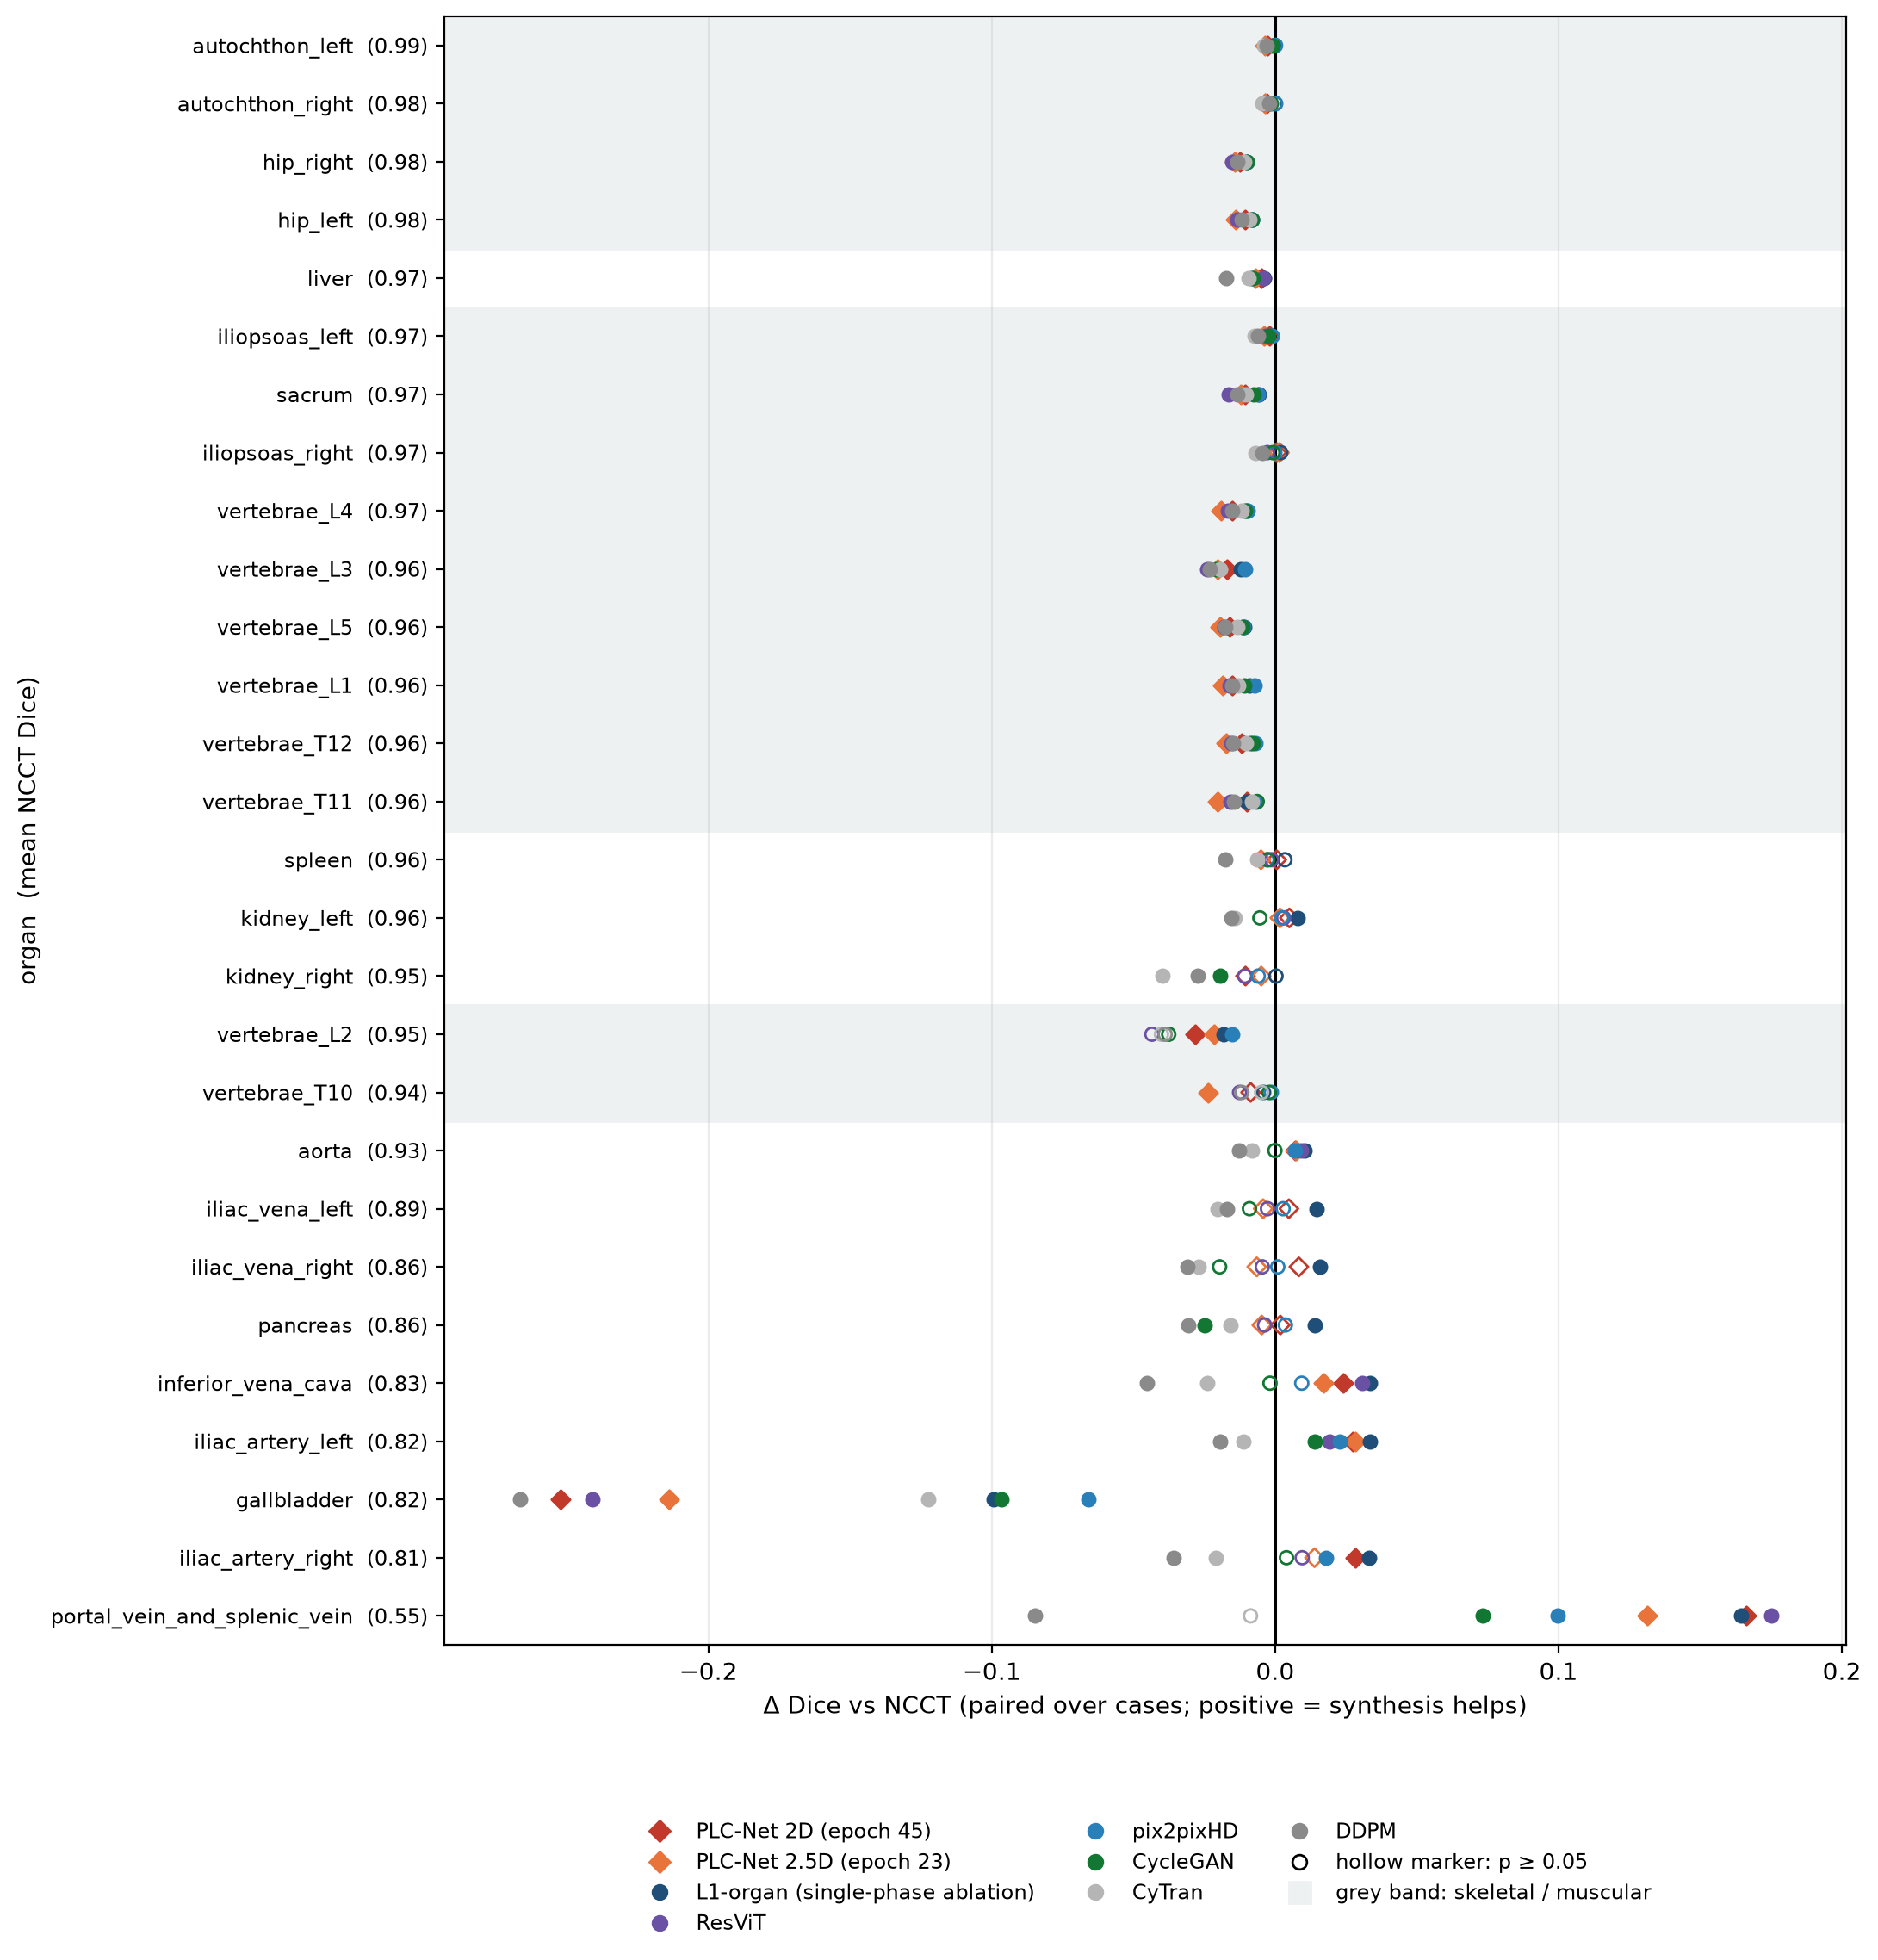
\includegraphics[width=0.95\textwidth]{synthesis/fig1_per_organ_effect.png}
\caption{تغییر دایس هر اندام نسبت به بازوی \lr{NCCT}، به‌صورت زوجی روی مواردی که اندام در هر دو بازو وجود دارد. عدد داخل پرانتز دایس میانگین \lr{NCCT} است؛ لوزی‌ها دو نسخه‌ی \lr{PLC-Net}اند، نشانگر توخالی یعنی $p \geq 0.05$، و نوار خاکستری اندام‌های اسکلتی و عضلانی را مشخص می‌کند.}
\label{fig:syn-organ}
\end{figure}

\begin{figure}[H]
\centering
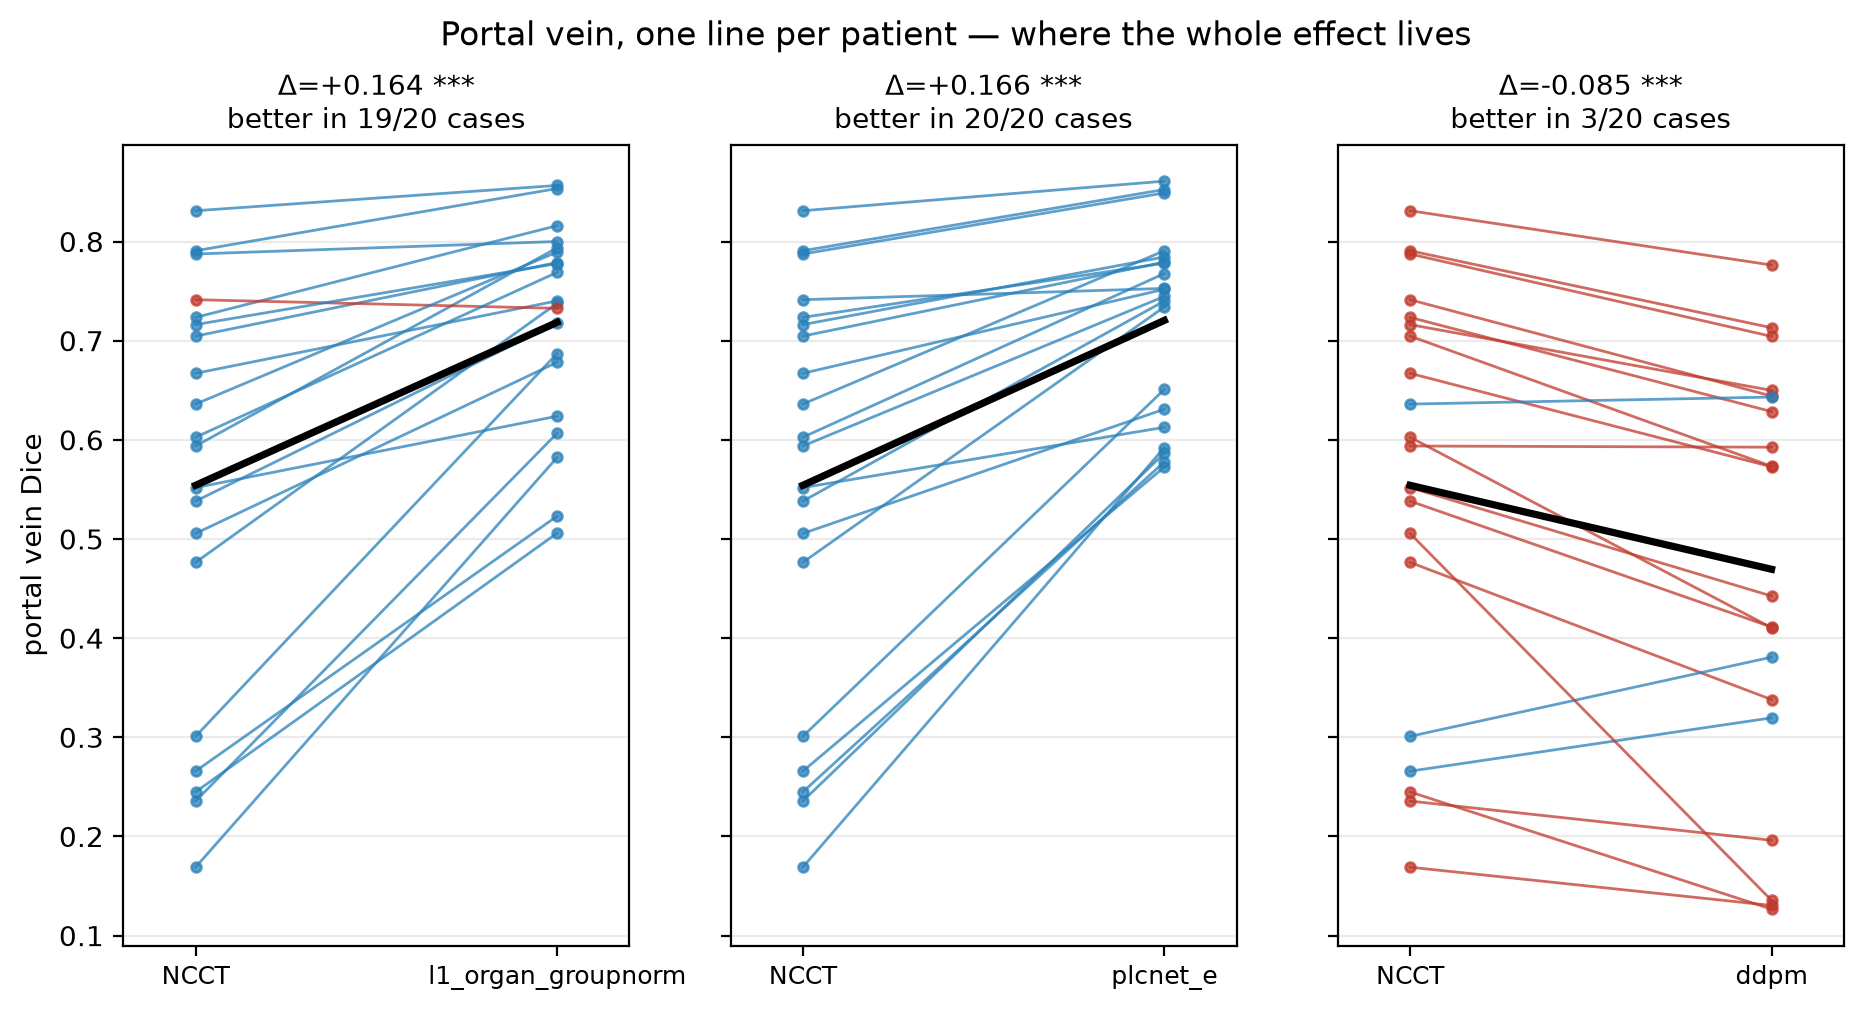
\includegraphics[width=0.95\textwidth]{synthesis/fig6_portal_vein_paired.png}
\caption{دایس ورید باب و طحالی برای هر بیمار، روی تصویر بدون‌تزریق (چپ هر نمودار) و روی خروجی مدل (راست)؛ خط سیاه میانگین است. \lr{PLC-Net} دوبعدی در \عدد{۲۰} مورد، \lr{L1}-اندام در \عدد{۱۹} مورد و \lr{DDPM} تنها در \عدد{۳} مورد از \عدد{۲۰} مورد دایس بالاتری از \lr{NCCT} دارند.}
\label{fig:syn-pv}
\end{figure}

\textbf{هزینه‌ی تولید.} همه‌ی بازوهای هم‌نهاده روی آناتومی اسکلتی دایس از دست می‌دهند: میان \عدد{−۰٫۰۰۸} و \عدد{−۰٫۰۲۱}، در همه‌ی بازوها معنادار ($p < 0.005$). چون استخوان با ماده‌ی حاجب تغییر نمی‌کند، این افت را می‌توان به خودِ فرایند تولید (تاری، تغییر بافت و آرتیفکت) نسبت داد.

\textbf{اثر خالص.} اثر خالص هر بازو، تفاوت دایس گروه عروقی منهای تفاوت دایس گروه اسکلتی همان بازو است. چون تفاوت اسکلتی منفی است، اثر خالص از سود خام عروقی بزرگ‌تر است؛ این کمیت سود عروقی را نسبت به افت عمومی همان بازو می‌سنجد و فرض می‌کند هزینه‌ی تولید بر عروق و استخوان به اندازه‌ی مشابه اثر می‌گذارد، فرضی که مستقیماً آزموده نشده است. در میان \عدد{۲۰} بازوی وریدی، افت اسکلتی و سود عروقی هم‌بستگی معناداری ندارند (اسپیرمن $\rho = +0.42$، $p = 0.07$) و افت اسکلتی تنها در بازه‌ای \عدد{۲٫۵} برابری تغییر می‌کند؛ با این تعداد بازو، این آزمون تنها وابستگی قوی را رد می‌کند (شکل~\ref{fig:syn-tax}).

\begin{figure}[H]
\centering
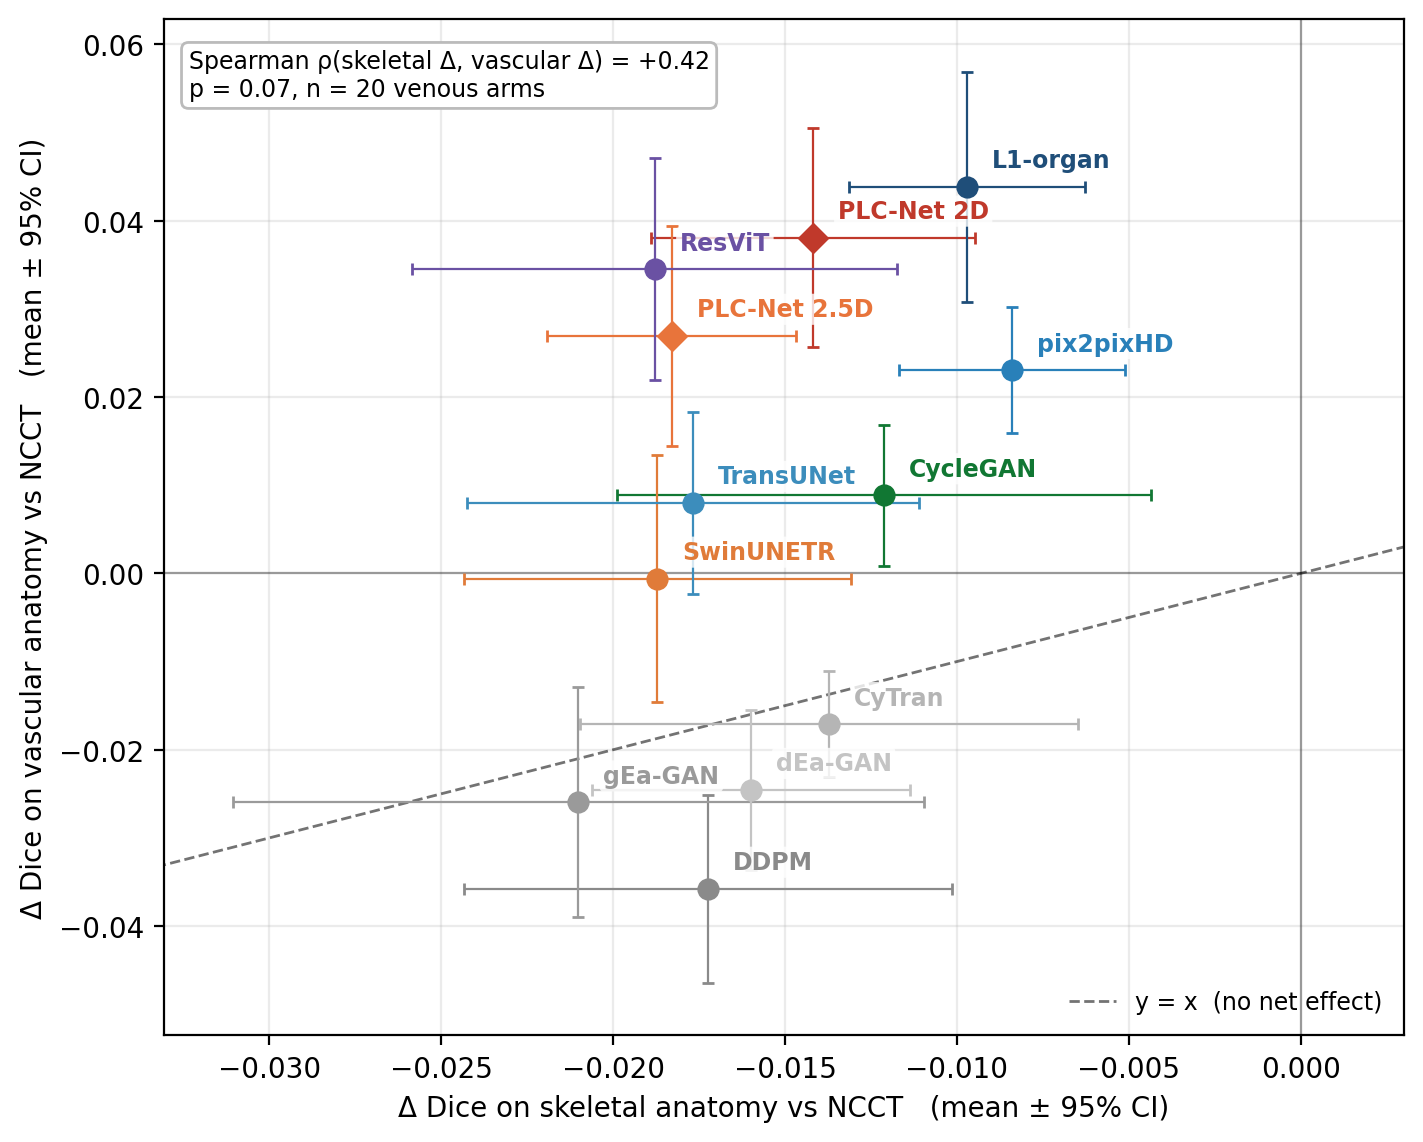
\includegraphics[width=0.8\textwidth]{synthesis/fig4_tax_vs_gain.png}
\caption{تغییر دایس گروه اسکلتی (افقی) در برابر تغییر دایس گروه عروقی (عمودی) نسبت به \lr{NCCT}، با فاصله‌ی اطمینان \عدد{۹۵} درصد، برای بازوهای جدول~\ref{tab:syn-gap}. روی خط‌چین $y = x$ سود عروقی با افت اسکلتی برابر است و فاصله‌ی عمودی هر نقطه از آن، اثر خالص است. هم‌بستگی اسپیرمن روی هر \عدد{۲۰} بازوی وریدی محاسبه شده است.}
\label{fig:syn-tax}
\end{figure}

\textbf{بازوهای با اثر خالص منفی.} \lr{CyTran}، \lr{gEa-GAN}، \lr{dEa-GAN} و \lr{DDPM} بخش‌بندی عروقی را بدتر می‌کنند و هیچ‌یک ورید باب را به‌طور معنادار بهبود نمی‌دهد. همین بازوها در \lr{featHU} نیز ضعیف‌ترند (\عدد{۳۸٫۱}، \عدد{۲۳٫۵}، \عدد{۲۵٫۲} و \عدد{۲۴٫۸}) و \lr{CyTran} دقت پویش \عدد{۰٫۳۵} دارد. \lr{SwinUNETR} و \lr{TransUNet} ورید باب را بهبود می‌دهند اما اثرشان بر کل گروه عروقی معنادار نیست. در مقایسه‌ی زوجی، \lr{PLC-Net} دوبعدی از هر چهار بازوی اخیر در گروه عروقی در همه‌ی \عدد{۲۰} مورد بالاتر است (\عدد{+۰٫۰۳۰} تا \عدد{+۰٫۰۶۴}، $p < 0.0001$ خام)؛ این چهار مقایسه در جدول~\ref{tab:syn-baselines}، که پیش از آزمایش به پنج روش محدود شده بود، وارد نشده‌اند.

\textbf{نقطه‌ی پایانی از پیش تعیین‌شده.} ترکیب اندام‌های وابسته به ماده‌ی حاجب دو اثر مخالف را در یک عدد جمع می‌کند و نتیجه تقریباً صفر است: تفاوت \lr{PLC-Net} دوبعدی با \lr{NCCT} برابر \عدد{+۰٫۰۰۱۱} است ($p = 0.94$، بالاتر در \عدد{۹} مورد از \عدد{۲۰})، در حالی که کمینه‌ی اثر قابل‌تشخیص در توان \عدد{۸۰} درصد حدود \عدد{۰٫۰۴۳} است. فرضیه‌ی تأییدی بنابراین از داده پشتیبانی نمی‌شود. تحلیل اندام‌به‌اندام نشان می‌دهد این حاصل جمعِ یک اثر مثبت بزرگ روی ورید باب و یک افت متمرکز روی کیسه‌ی صفراست. یافته‌های ورید باب، چون از پیش به‌عنوان نقطه‌ی پایانی تعیین نشده بودند، اکتشافی شمرده می‌شوند.

\subsection*{مقایسه با روش‌های منتشرشده}

جدول~\ref{tab:syn-baselines} \lr{PLC-Net} دوبعدی را به‌صورت زوجی با چهار روش منتشرشده و با مدل انتشار \lr{DDPM} مقایسه می‌کند.

\begin{table}[H]
\centering
\footnotesize
\caption{مقایسه‌ی زوجی \lr{PLC-Net} دوبعدی با سایر مدل‌ها روی داده و تقسیم یکسان؛ مقادیر مثبت یعنی دایس \lr{PLC-Net} بالاتر است. مقادیر $p$ با روش هولم روی \عدد{۳۰} آزمون تصحیح شده‌اند (پنج مقایسه در شش نقطه‌ی پایانی: گروه عروقی، ورید باب، ترکیب وابسته به ماده‌ی حاجب، و گروه‌های پارانشیمی، اسکلتی و عضلانی).}
\label{tab:syn-baselines}
\begin{tabular}{|p{2.3cm}|c|c|c|c|p{3.4cm}|}
\hline
\textbf{در برابر} & \textbf{$\Delta$ عروقی} & \textbf{$p$ هولم} & \textbf{$\Delta$ ورید باب} & \textbf{$p$ هولم} & \textbf{نتیجه} \\
\hline
\lr{ResViT} & \عدد{+۰٫۰۰۳۶} & \عدد{۱٫۰۰} & \عدد{−۰٫۰۰۸۶} & \عدد{۱٫۰۰} & هم‌ارز در حاشیه‌ی $\pm 0.02$ \\
\hline
\lr{pix2pixHD} & \عدد{+۰٫۰۱۵۰} & \عدد{۰٫۰۱۳} & \عدد{+۰٫۰۶۶۶} & \عدد{۰٫۰۱۳} & \lr{PLC-Net} بالاتر \\
\hline
\lr{CycleGAN} & \عدد{+۰٫۰۲۹۲} & \عدد{۰٫۰۰۰۴} & \عدد{+۰٫۰۹۳۰} & \عدد{۰٫۰۰۰۳} & \lr{PLC-Net} بالاتر \\
\hline
\lr{CyTran} & \عدد{+۰٫۰۵۵۲} & $<0.0001$ & \عدد{+۰٫۱۷۵۰} & $<0.0001$ & \lr{PLC-Net} بالاتر \\
\hline
\lr{DDPM} & \عدد{+۰٫۰۷۳۹} & $<0.0001$ & \عدد{+۰٫۲۵۱۰} & $<0.0001$ & \lr{PLC-Net} بالاتر \\
\hline
\end{tabular}
\end{table}

\textbf{\lr{ResViT}.} تفاوت با \lr{ResViT} معنادار نیست ($p$ خام برابر \عدد{۰٫۳۸}). با \عدد{۲۰} مورد، کمینه‌ی تفاوت قابل‌تشخیص برای این مقایسه‌ی زوجی در گروه عروقی و در توان \عدد{۸۰} درصد حدود \عدد{۰٫۰۱۲} دایس است. آزمون هم‌ارزی دوطرفه (\lr{TOST}) هم‌ارزی را در حاشیه‌ی $\pm 0.02$ دایس تأیید می‌کند ($p = 0.0003$) اما در حاشیه‌ی $\pm 0.01$ نه ($p = 0.060$). نتیجه‌ی دقیق این است که دو مدل در حاشیه‌ی \عدد{۰٫۰۲} دایس هم‌ارزند و تفاوتی در حد \عدد{۰٫۰۱} را نمی‌توان رد کرد. تمایز \lr{PLC-Net} با \lr{ResViT} در دقت پایین‌دستی نیست، بلکه در کنترل پویش است: \lr{ResViT}، مانند سایر مدل‌های این جدول، تک‌پویش است و برای هر پویش باید جداگانه آموزش ببیند، در حالی که \lr{PLC-Net} هر دو پویش را با یک مدل تولید می‌کند. تمایز دوم در اندازه‌ی مدل و حافظه است که در زیربخش بعد می‌آید.

مقایسه با مبنای حذفی داخلی \lr{L1}-اندام، که نه شرط دارد و نه جمله‌ی تخاصمی، در بخش~\ref{sec:e-ablation} می‌آید: نتیجه نشان می‌دهد بخش عمده‌ی سود پایین‌دستی را می‌توان به زیان \lr{L1} وزن‌دار اندامی نسبت داد و نه به اجزای شرطی، اما آن مبنا قادر به تولید پویش شریانی نیست و برای هر پویش باید مدلی جداگانه آموزش ببیند. سهم \lr{PLC-Net} در همین‌جاست: یک مدل واحد، هر دو پویش را با کنترل صریح تولید می‌کند و سودمندی پایین‌دستی آن با بهترین مدل‌های تک‌پویش برابر می‌ماند؛ یعنی کنترل پویش و سطح بدون هزینه‌ی دقت به دست می‌آید.

\subsection*{هزینه‌ی محاسباتی}
\label{sec:e-syn-cost}

دو مدل با سودمندی هم‌ارز می‌توانند هزینه‌ی بسیار متفاوتی داشته باشند، و جدول~\ref{tab:syn-baselines} همین حالت را میان \lr{PLC-Net} و \lr{ResViT} نشان داد. جدول~\ref{tab:syn-cost} هزینه‌ی مولد هر مدل را با رویه‌ی بخش~\ref{sec:e-setup-cost} گزارش می‌کند. هر سه کمیت پراسنجه، شمار عمل و حافظه به بار پردازنده‌ی گرافیکی بستگی ندارند؛ زمان واقعی گزارش نمی‌شود.

\begin{table}[H]
\centering
\footnotesize
\caption{هزینه‌ی مولد هر مدل. «شمار عمل، $256\times256$» شمار عمل یک اجرای مولد روی برش $256\times256$ است (برای مدل انتشار، یک اجرای شبکه). «ورودی ارزیابی» ورودی یک اجرا در ارزیابی این پایان‌نامه است. «اجرا به‌ازای هر برش» شمار اجراهای لازم برای یک برش است (\عدد{۱۶} وصله؛ برای مدل انتشار \عدد{۱۶} وصله در \عدد{۲۵} گام)، و «شمار عمل به‌ازای هر برش» حاصل‌ضرب شمار عمل یک اجرا روی ورودی ارزیابی در آن است. حافظه برای یک اجرا روی ورودی ارزیابی با دسته‌ی یک است. در ستون‌های پراسنجه، شمار عمل (هر دو ستون) و حافظه، کمترین مقدار پررنگ و دومین مقدار کمتر زیرخط‌دار است.}
\label{tab:syn-cost}
\begin{tabular}{|p{2.3cm}|C{1.4cm}|C{1.7cm}|C{1.8cm}|C{1.4cm}|C{1.8cm}|C{1.5cm}|}
\hline
\textbf{مدل} & \textbf{پراسنجه (میلیون)} & \textbf{شمار عمل، $256\times256$ (میلیارد)} & \textbf{ورودی ارزیابی} & \textbf{اجرا به‌ازای هر برش} & \textbf{شمار عمل به‌ازای هر برش (میلیارد)} & \textbf{حافظه (مگابایت)} \\
\hline
\multicolumn{7}{|l|}{\emph{مدل پیشنهادی}} \\
\hline
\lr{PLC-Net} دوبعدی & \عدد{۱۳٫۵۵} & \عدد{۲۹٫۸} & وصله‌ی $128\times128$ & \عدد{۱۶} & \عدد{۱۱۹٫۴} & \عدد{۱۴۵} \\
\hline
\lr{PLC-Net} \عدد{۲٫۵}~بعدی & \عدد{۱۳٫۵۶} & \عدد{۳۰٫۲} & وصله‌ی $128\times128$ & \عدد{۱۶} & \عدد{۱۲۱٫۰} & \عدد{۱۴۸} \\
\hline
\multicolumn{7}{|l|}{\emph{روش‌های منتشرشده}} \\
\hline
\lr{pix2pixHD} & \عدد{۱۳٫۳۲} & \عدد{۲۹٫۸} & وصله‌ی $128\times128$ & \عدد{۱۶} & \عدد{۱۱۹٫۲} & \underline{\عدد{۱۳۵}} \\
\hline
\lr{CycleGAN} & \underline{\عدد{۱۱٫۳۷}} & \عدد{۴۸٫۹} & برش $256\times256$ & \عدد{۱} & \عدد{۴۸٫۹} & \عدد{۱۳۹} \\
\hline
\lr{ResViT} & \عدد{۱۲۳٫۴۴} & \عدد{۱۱۹٫۸} & برش $256\times256$ & \عدد{۱} & \عدد{۱۱۹٫۸} & \عدد{۱۰۰۴} \\
\hline
\lr{CyTran} & \textbf{\عدد{۱٫۱۹}} & \textbf{\عدد{۲٫۰}} & برش $256\times256$ & \عدد{۱} & \textbf{\عدد{۲٫۰}} & \textbf{\عدد{۳۸}} \\
\hline
\lr{SwinUNETR} & \عدد{۲۵٫۱۴} & \عدد{۱۸٫۱} & برش $256\times256$ & \عدد{۱} & \عدد{۱۸٫۱} & \عدد{۳۱۸} \\
\hline
\lr{TransUNet} & \عدد{۱۰۵٫۳۲} & \عدد{۳۸٫۵} & برش $256\times256$ & \عدد{۱} & \عدد{۳۸٫۵} & \عدد{۸۶۷} \\
\hline
\lr{gEa-GAN} & \عدد{۴۱٫۸۳} & \underline{\عدد{۵٫۹}} & برش $256\times256$ & \عدد{۱} & \underline{\عدد{۵٫۹}} & \عدد{۳۴۶} \\
\hline
\lr{dEa-GAN} & \عدد{۴۱٫۸۳} & \underline{\عدد{۵٫۹}} & برش $256\times256$ & \عدد{۱} & \underline{\عدد{۵٫۹}} & \عدد{۳۴۶} \\
\hline
\multicolumn{7}{|l|}{\emph{مدل انتشار}} \\
\hline
\lr{DDPM} & \عدد{۱۳٫۷۹} & \عدد{۲۹٫۹} & وصله‌ی $128\times128$ & \عدد{۴۰۰} & \عدد{۲۹۸۸} & \عدد{۱۴۷} \\
\hline
\end{tabular}
\end{table}

\مهم{با ورودی یکسان، \lr{PLC-Net} بسیار سبک‌تر از \lr{ResViT} است.} روی یک برش $256\times256$، \lr{ResViT} حدود \عدد{۹} برابر پراسنجه (\عدد{۱۲۳٫۴۴} در برابر \عدد{۱۳٫۵۵} میلیون) و حدود \عدد{۴} برابر شمار عمل (\عدد{۱۱۹٫۸} در برابر \عدد{۲۹٫۸} میلیارد) دارد. افزون بر این، \lr{ResViT} تک‌پویش است و پوشش هر دو پویش دو مدل جداگانه می‌خواهد؛ با فرض این‌که نسخه‌ی شریانی همان معماری را داشته باشد، پراسنجه‌ی لازم حدود \عدد{۲۴۷} میلیون می‌شود، یعنی حدود \عدد{۱۸} برابر \lr{PLC-Net}. این رقم محاسبه‌ای است و اندازه‌گیری نیست.

\مهم{در ارزیابی، شمار عمل به‌ازای هر برش برابر می‌شود.} \lr{PLC-Net} هر برش را در \عدد{۱۶} وصله‌ی هم‌پوشان می‌پردازد، که هر نقطه‌ی برش را حدود \عدد{۳٫۷} بار می‌پوشانند (برای مورد آزمونی با اندازه‌ی میانه). شمار عمل آن به‌ازای هر برش \عدد{۱۱۹٫۴} میلیارد می‌شود، برابر \lr{ResViT} (\عدد{۱۱۹٫۸}) که هر برش را یک‌بار می‌پردازد؛ یعنی مزیت حدود چهاربرابری شمار عمل یک اجرا در ارزیابی به کاشی‌کاری هم‌پوشان می‌رسد. اندازه‌ی مدل و حافظه چنین نیستند: یک اجرای \lr{PLC-Net} روی یک وصله \عدد{۱۴۵} مگابایت می‌خواهد، در برابر \عدد{۱۰۰۴} مگابایت برای \lr{ResViT} (حدود \عدد{۷} برابر کمتر). پس مزیت \lr{PLC-Net} نسبت به \lr{ResViT} در اندازه‌ی مدل و حافظه است و نه در شمار عمل ارزیابی؛ زمان تولید یک حجم در این پایان‌نامه اندازه‌گیری نشده است.

\مهم{شش مدل تک‌گذر شمار عمل کمتری از \lr{PLC-Net} دارند و هیچ‌یک سودمندی آن را ندارد.} در ارزیابی، \lr{CyTran} (\عدد{۲٫۰} میلیارد عمل به‌ازای هر برش)، دو مدل \lr{Ea-GAN} (\عدد{۵٫۹})، \lr{SwinUNETR} (\عدد{۱۸٫۱})، \lr{TransUNet} (\عدد{۳۸٫۵}) و \lr{CycleGAN} (\عدد{۴۸٫۹}) همگی کمتر از \lr{PLC-Net} (\عدد{۱۱۹٫۴}) دارند. اثر خالص این شش مدل در جدول~\ref{tab:syn-gap} از \عدد{−۰٫۰۰۸۵} تا \عدد{+۰٫۰۲۶} است، در برابر \عدد{+۰٫۰۵۲} برای \lr{PLC-Net}؛ یعنی در میان این شش مدل، شمار عمل کمتر با سودمندی کمتر همراه بوده است. این همراهی علیت نیست و تنها چند مدل را در بر می‌گیرد. \lr{pix2pixHD} و \lr{ResViT} شمار عمل برابر با \lr{PLC-Net} دارند (\عدد{۱۱۹٫۲} و \عدد{۱۱۹٫۸})؛ سودمندی \lr{ResViT} با \lr{PLC-Net} هم‌ارز و سودمندی \lr{pix2pixHD} کمتر است (جدول~\ref{tab:syn-baselines})، پس در شمار عمل برابر، \lr{PLC-Net} از هیچ‌یک سودمندی کمتری ندارد. نسخه‌ی \عدد{۲٫۵}~بعدی با ورودی \عدد{۱۱} برش تقریباً همان هزینه را دارد (\عدد{۱۲۱٫۰} در برابر \عدد{۱۱۹٫۴} میلیارد عمل)، پس هزینه دلیل انتخاب نسخه‌ی دوبعدی نبوده است.

\مهم{مدل انتشار.} \lr{DDPM} در هر اجرای شبکه \عدد{۲۹٫۹} میلیارد عمل دارد و در ارزیابی هر برش \عدد{۴۰۰} اجرا می‌خواهد (\عدد{۱۶} وصله در \عدد{۲۵} گام)، یعنی \عدد{۲۹۸۸} میلیارد عمل به‌ازای هر برش: \عدد{۲۵} برابر \lr{PLC-Net}، با اثر خالص منفی (جدول~\ref{tab:syn-gap}). پراسنجه‌ی آن (\عدد{۱۳٫۷۹} میلیون) هم‌اندازه‌ی \lr{PLC-Net} است؛ هزینه‌ی آن از نمونه‌برداری می‌آید و نه از اندازه‌ی شبکه.

\مهم{دامنه‌ی جدول.} شمار عمل به‌ازای هر برش هزینه‌ی تولید یک حجم را از روی شمار برش (میانگین \عدد{۲۷۲٫۹}) می‌دهد، اما زمان واقعی را نه؛ زمان به کارایی هسته‌ها، اندازه‌ی دسته و پهنای باند حافظه هم بستگی دارد و اندازه‌گیری نشده است. هزینه‌ی آموزش نیز سنجیده نشد. شمار وصله‌ی \lr{PLC-Net} به هم‌پوشانی ارزیابی وابسته است؛ کم‌کردن آن شمار عمل را کم می‌کند، اما اثرش بر کیفیت خروجی آزموده نشده است. جدول بنابراین هزینه‌ی ارزیابیِ گزارش‌شده را نشان می‌دهد و نه کمینه‌ی هزینه‌ی ممکن این مدل.

\subsection*{مقایسه‌ی بصری}

برای انتخاب مورد نمایش، همه‌ی \عدد{۲۰} مورد آزمون بر پایه‌ی ارقام کمّی هر مورد مرتب شدند (سود ورید باب نسبت به \lr{NCCT}، فاصله از بهترین روش منتشرشده، فاصله‌ی \lr{featHU} از \lr{ResViT} و پاسخ پویش). شکل~\ref{fig:syn-cmp} موردی را نشان می‌دهد که سود ورید باب و فاصله‌ی آن از بهترین روش منتشرشده در آن به میانه‌ی موارد آزمون نزدیک‌ترند؛ یعنی یک بیمار نمونه، و نه بهترین مورد. برش در ترازی انتخاب شده است که ورید باب و طحالی در آن بیشترین سطح را دارد.

در هر ستون، خطوط رنگی خروجی \lr{TotalSegmentator} روی \emph{همان} تصویر آن ستون است و عدد پایین هر تصویر بزرگ‌نمایی‌شده، دایس حجمی ورید باب و کیسه‌ی صفرای همان مورد نسبت به مرجع است. در تصویر با ماده‌ی حاجب واقعی ورید طحالی به‌صورت یک ساختار روشن و پیوسته دیده می‌شود؛ روی تصویر بدون‌تزریق، بخش‌بند تنها قطعه‌ای از آن را می‌یابد (دایس \عدد{۰٫۶۰}). \lr{PLC-Net} دوبعدی (\عدد{۰٫۷۷})، \lr{ResViT} (\عدد{۰٫۷۸}) و \lr{L1}-اندام (\عدد{۰٫۷۷}) بخش بزرگ‌تری از ورید را بازمی‌گردانند، هرچند هیچ‌یک طول کامل ورید طحالی را بازسازی نمی‌کند؛ \lr{pix2pixHD} و \lr{CycleGAN} در میانه‌اند (\عدد{۰٫۶۹} و \عدد{۰٫۶۷}) و \lr{CyTran} و \lr{DDPM} از کف \lr{NCCT} پایین‌ترند (\عدد{۰٫۵۷} و \عدد{۰٫۴۱}). تفاوت بافت نیز دیده می‌شود: خروجی \lr{L1}-اندام و \lr{DDPM} به‌طور محسوس هموارتر از تصویر واقعی است، در حالی که بافت \lr{PLC-Net} دوبعدی به تصویر واقعی نزدیک‌تر است، که با نسبت طیفی آن (\عدد{۰٫۹۸۲} در برابر \عدد{۰٫۸۴۲} برای \lr{L1}-اندام) سازگار است. در ردیف تفاوت، آبی گسترده روی کبد در خروجی \lr{CyTran} و \lr{PLC-Net} \عدد{۲٫۵}~بعدی نشانه‌ی کم‌تقویتی پارانشیم است.

\begin{figure}[H]
\centering
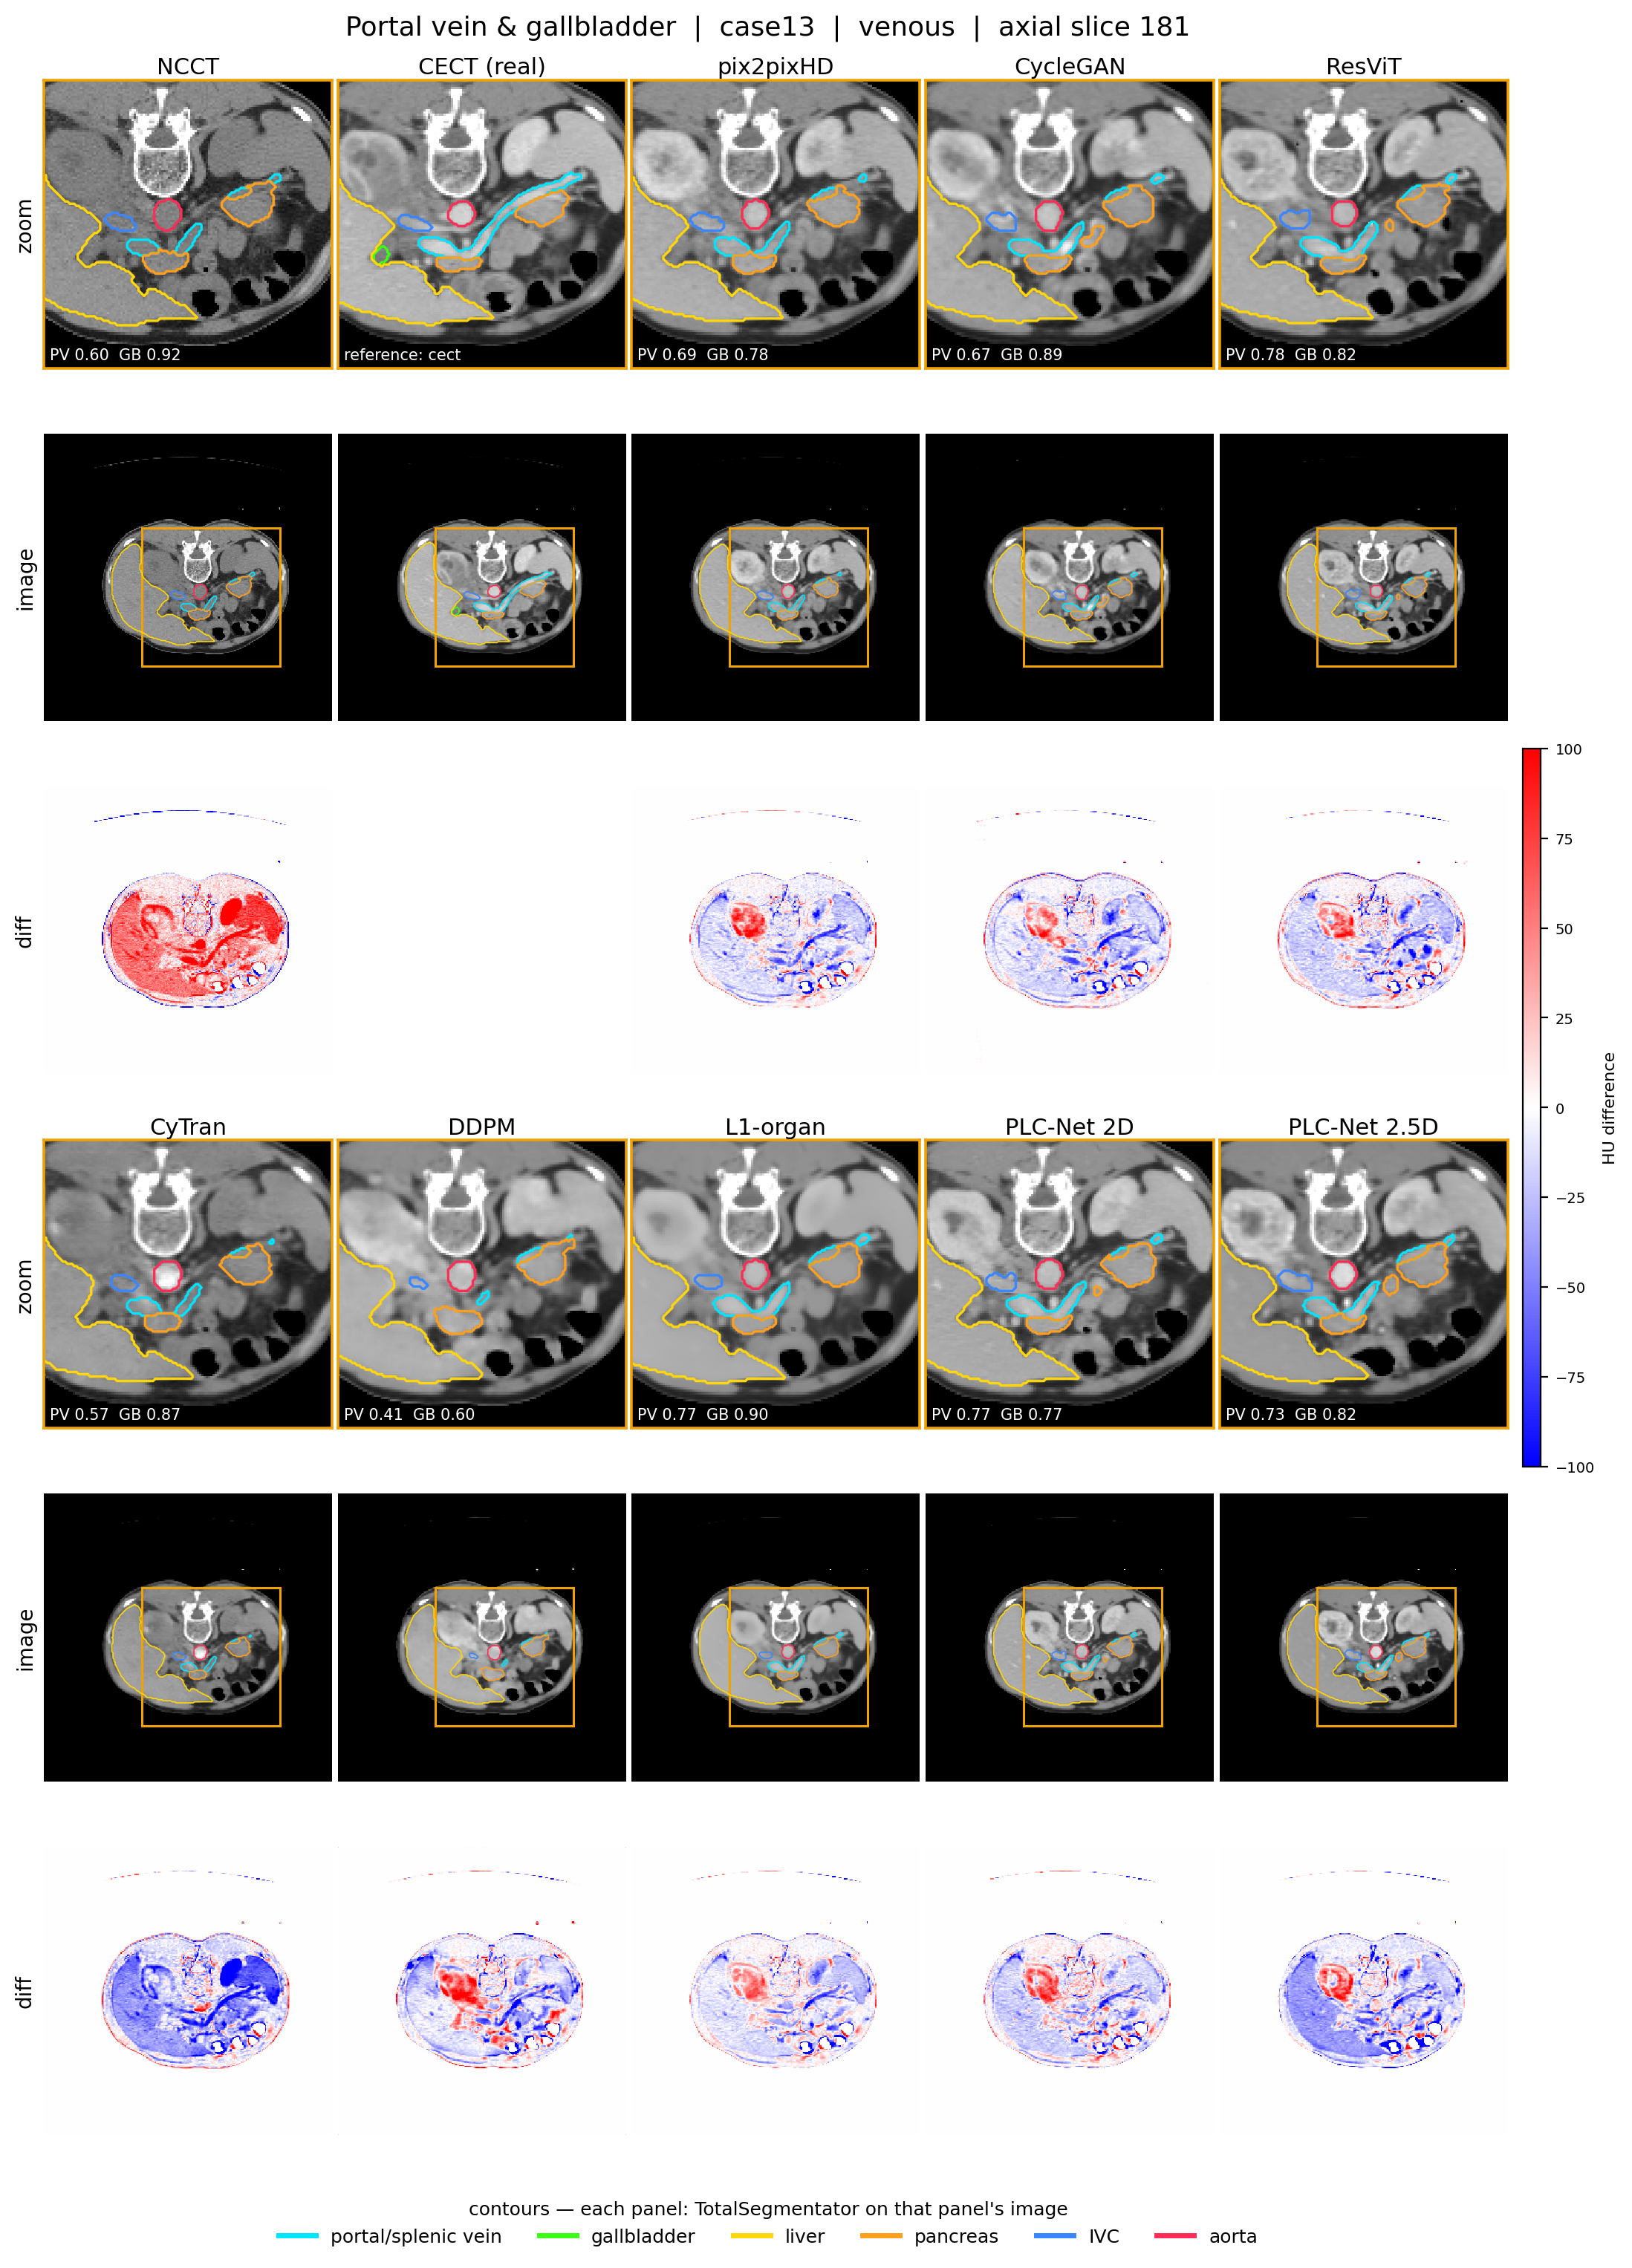
\includegraphics[width=\textwidth,height=0.72\textheight,keepaspectratio]{synthesis/qual_venous_case13.png}
\caption{مقایسه‌ی بصری در پویش وریدی برای یک مورد آزمون نمونه (نزدیک به میانه‌ی سود ورید باب)، در تراز ورید باب. ردیف بزرگ‌نمایی و ردیف تصویر: پنجره‌ی $W = 400$، $L = 40$؛ خطوط رنگی، بخش‌بندی \lr{TotalSegmentator} روی تصویر همان ستون؛ عدد پایین هر تصویر بزرگ‌نمایی‌شده، دایس حجمی ورید باب (\lr{PV}) و کیسه‌ی صفرا (\lr{GB}) نسبت به مرجع. ردیف تفاوت: پس از محدودسازی هر دو تصویر به بازه‌ی $[-200, 400]$ واحد هانسفیلد، با مقیاس $\pm 100$ واحد؛ در ستون \lr{NCCT} تصویر با ماده‌ی حاجب واقعی منهای تصویر بدون‌تزریق، و در ستون هر مدل خروجی مدل منهای تصویر با ماده‌ی حاجب واقعی (قرمز: روشن‌تر، آبی: تیره‌تر).}
\label{fig:syn-cmp}
\end{figure}

\section{مطالعه‌ی حذفی}
\label{sec:e-ablation}

این بخش نشان می‌دهد کدام جزء روش نتیجه‌ی بخش~\ref{sec:e-syn} را ساخته است. نخست زنجیره‌ی پیکربندی‌های \lr{PLC-Net} (بخش~\ref{sec:m-syn}) گزارش می‌شود و سپس دو مطالعه‌ی حذفی مؤلفه‌ی هم‌ترازسازی (بخش~\ref{sec:m-reg}): سهم هر گام پیش‌پردازش و مقایسه‌ی توابع هدف.

\subsection*{مطالعه‌ی حذفی \lr{PLC-Net}: زنجیره‌ی پیکربندی‌ها}


معماری نهایی حاصل شش پیکربندی پیاپی است که هر یک در پاسخ به رفتار مشاهده‌شده‌ی پیکربندی پیش از خود ساخته شد. جدول~\ref{tab:syn-path} هر پیکربندی را با تغییر اصلی و هدف طراحی‌اش فهرست می‌کند؛ ارقام همه‌ی پیکربندی‌ها در جدول~\ref{tab:syn-ablation} آمده است.

\begin{table}[H]
\centering
\footnotesize
\caption{مسیر طراحی \lr{PLC-Net}: تغییر اصلی و هدف طراحی هر پیکربندی.}
\label{tab:syn-path}
\begin{tabular}{|p{2.8cm}|p{5.3cm}|p{6.2cm}|}
\hline
\textbf{پیکربندی} & \textbf{تغییر اصلی} & \textbf{هدف طراحی} \\
\hline
نقطه‌ی شروع & \lr{U-Net} دوبعدی روی وصله‌های $128\times128$، آموزش‌دیده تنها روی جفت‌های پویش وریدی & آغاز با کوچک‌ترین مدل ممکن: پس از پالایه (\lr{filter}) کیفیت هم‌ترازی تنها حدود صد جفت حجمی در دسترس است و یک شبکه‌ی سه‌بعدی با این حجم داده به‌سرعت بیش‌برازش می‌کند \\
\hline
\lr{A}: چندپویشی بدون شرط & افزودن جفت‌های پویش شریانی به استخر آموزش & دو برابر کردن داده؛ بدون سازوکاری برای انتخاب میان دو هدف، مدل ناگزیر میان آن‌ها میانگین می‌گیرد \\
\hline
\lr{B}: شرط پویش & بردار شناسه‌ی پویش (\عدد{۶۴}~بعدی) از طریق \lr{FiLM}~\cite{perez2018film} به رمزگشا داده می‌شود & کم‌هزینه‌ترین راه برای رفع ابهام هدف، بی‌آن‌که مزیت استخر دوبرابری از دست برود \\
\hline
\lr{C}: جمله‌ی متخاصم با ضریب متعارف & افزودن متمایزکننده با $\lambda_{\text{adv}}=2.0$ & افزودن واقع‌نمایی بافتی با ضریب پیش‌فرض ادبیات \\
\hline
\lr{D}: زمینه‌ی محور $z$ & پیکربندی \عدد{۲٫۵}~بعدی: $2k+1$ برش مجاور به‌عنوان مجرای (\lr{channel}) ورودی و پیش‌بینی برش میانی & بازگرداندن بافت و انسجام بین‌برشی، بدون بازگشت به ضریب متخاصم پایین؛ شبکه دوبعدی می‌ماند و تعداد پراسنجه‌ها تقریباً ثابت است \\
\hline
\lr{E}: شرط سطح و ضریب متخاصم کالیبره & $\lambda_{\text{adv}}=0.5$، تطبیق ویژگی (\lr{feature matching})، نرمال‌سازی گروهی، و بردار \emph{سطح تقویت} در سطح اندام به‌عنوان شرط & کالیبره‌کردن جمله‌ی متخاصم و افزودن دومین علامت کنترل. چون چند تغییر هم‌زمان‌اند، اثر این گام را نمی‌توان تنها به شرط سطح نسبت داد \\
\hline
\lr{F}: شرط سطح به‌علاوه‌ی زمینه‌ی $z$ & ترکیب \lr{E} با ورودی \عدد{۲٫۵}~بعدی & بهره‌گیری هم‌زمان از شرط سطح و زمینه‌ی محور $z$ \\
\hline
\end{tabular}
\end{table}

منطق رسیدن به معماری نهایی از این جدول چنین خوانده می‌شود. مدل شرطی چندپویشی، با شرط پویش، هم‌زمان دو مزیت می‌گیرد: استخر آموزشی دو برابر می‌شود \emph{و} خروجی مبهم نمی‌ماند؛ تعداد جفت‌های قابل‌استفاده از \عدد{۹۷} به \عدد{۱۹۳} جفت حجمی می‌رسد، که با بیش‌برازش اجراهای تک‌پویش روی این داده‌ی کوچک مقابله می‌کند. جمله‌ی متخاصم و زمینه‌ی محور $z$ برای بازگرداندن بافت افزوده شدند، و شرط سطح برای در اختیار گرفتن تغییرپذیری تقویت بیمار به بیمار. مشاهدات هر گام پس از جدول~\ref{tab:syn-ablation} می‌آید.

\مهم{مدل نهایی این پایان‌نامه، پیکربندی دوبعدی \lr{E} با وزن‌های دوره‌ی \عدد{۴۵} است.} این پیکربندی تنها پیکربندی‌ای است که هر دو علامت کنترل، یعنی شرط پویش و شرط سطح، را هم‌زمان نگه می‌دارد. شواهد این انتخاب، از جمله اثر پایین‌دستی آن در میان پیکربندی‌های شرطی، در همین بخش و در بخش~\ref{sec:e-analysis} آمده است. آموزش پیکربندی \lr{E} در دوره‌ی \عدد{۴۵} و پیکربندی \lr{F} در دوره‌ی \عدد{۵۳} متوقف شد؛ وزن‌های گزارش‌شده دوره‌ی \عدد{۴۵} برای \lr{E} و دوره‌ی \عدد{۲۳} برای \lr{F} است.

از این مسیر سه فرضیه‌ی طراحی بیرون می‌آید که در همین بخش و بخش~\ref{sec:e-syn} به‌صورت کمّی سنجیده می‌شوند: ضریب متخاصم در این مسئله یک فراپراسنجه‌ی حساس است؛ شرطی‌سازی پویش امکان آموزش یک مدل واحد روی جفت‌های هر دو پویش را فراهم می‌کند و بدین ترتیب داده‌ی آموزشی را دو برابر می‌کند؛ و دو علامت شرط (پویش و سطح) تا حد زیادی اطلاعات مشترک دارند، به‌طوری‌که شبکه می‌تواند یکی را به بهای دیگری نادیده بگیرد. این پدیده در بخش~\ref{sec:e-syn} اندازه‌گیری و تحلیل می‌شود.

جدول~\ref{tab:syn-ablation} و شکل~\ref{fig:syn-ladder} همین پیکربندی‌ها را مقایسه می‌کنند.

\begin{table}[H]
\centering
\footnotesize
\caption{پیکربندی‌های \lr{A} تا \lr{F} در پویش وریدی، هر یک با وزن‌های نماینده‌ی خود. اثر خالص با فاصله‌ی اطمینان \عدد{۹۵} درصد گزارش شده است. \lr{E} و \lr{F} در حالت سطح \lr{population} ($z = 0$) استنتاج شده‌اند. بهترین مقدار پررنگ و دومین مقدار بهتر زیرخط‌دار است.}
\label{tab:syn-ablation}
\begin{tabular}{|p{5.0cm}|c|c|c|c|}
\hline
\textbf{پیکربندی} & \lr{\textbf{featHU}}$\downarrow$ & \textbf{دقت پویش} & \lr{\textbf{FID}}$\downarrow$ & \textbf{اثر خالص} \\
\hline
\lr{A}: چندپویشی بدون شرط & \عدد{۱۹٫۳۹} & \عدد{۰٫۷۰} & \عدد{۲۲٫۴} & \عدد{+۰٫۰۳۳ $\pm$ ۰٫۰۱۱} \\
\hline
\lr{B}: \lr{A} + شرط پویش (\lr{FiLM}) & \textbf{\عدد{۱۴٫۲۶}} & \textbf{\عدد{۱٫۰۰}} & \عدد{۲۳٫۵} & \عدد{+۰٫۰۴۲ $\pm$ ۰٫۰۱۲} \\
\hline
\lr{C}: \lr{B} + جمله‌ی تخاصمی ($\lambda_{\text{adv}} = 2.0$) & \عدد{۳۵٫۰۱} & \underline{\عدد{۰٫۸۵}} & \عدد{۱۷٫۶} & \عدد{+۰٫۰۱۶ $\pm$ ۰٫۰۰۶} \\
\hline
\lr{D}: \lr{C} + ورودی \عدد{۱۱} برشی & \عدد{۱۸٫۷۵} & \textbf{\عدد{۱٫۰۰}} & \underline{\عدد{۱۵٫۲}} & \عدد{+۰٫۰۲۱ $\pm$ ۰٫۰۱۱} \\
\hline
\lr{E}: \lr{D} + شرط سطح، تخاصمی کالیبره؛ \lr{PLC-Net} دوبعدی & \underline{\عدد{۱۴٫۵۵}} & \textbf{\عدد{۱٫۰۰}} & \textbf{\عدد{۹٫۶}} & \textbf{\عدد{+۰٫۰۵۲ $\pm$ ۰٫۰۱۵}} \\
\hline
\lr{F}: \lr{E} + زمینه‌ی $z$؛ \lr{PLC-Net} \عدد{۲٫۵}~بعدی${}^{\dagger}$ & \عدد{۲۲٫۰۱} & \عدد{۰٫۷۵} & \عدد{۱۶٫۷} & \underline{\عدد{+۰٫۰۴۵ $\pm$ ۰٫۰۱۵}} \\
\hline
\end{tabular}
\end{table}

افزودن شرط پویش (\lr{A} به \lr{B}) دقت پویش را از \عدد{۰٫۷۰} به \عدد{۱٫۰۰} می‌رساند، \lr{featHU} را از \عدد{۱۹٫۴} به \عدد{۱۴٫۳} کاهش می‌دهد و اثر خالص را از \عدد{+۰٫۰۳۳} به \عدد{+۰٫۰۴۲} افزایش می‌دهد (مقایسه‌ی زوجی، $p = 0.009$). افزودن جمله‌ی تخاصمی با ضریب متعارف $\lambda_{\text{adv}} = 2.0$ (\lr{C}) اثر خالص را \عدد{۶۱} درصد کاهش می‌دهد (به \عدد{+۰٫۰۱۶}) و \lr{featHU} را به \عدد{۳۵٫۰} می‌رساند؛ این همان مشاهده‌ای است که انتخاب $\lambda_{\text{adv}} = 0.5$ در بخش~\ref{sec:m-syn} بر آن تکیه دارد. ورودی \عدد{۱۱} برشی (\lr{D}) بخشی از این افت را جبران می‌کند.

لاگ آموزش پیکربندی \lr{C} علت افت را نشان می‌دهد: زیان مولد بالا می‌رود در حالی که
زیان متمایزکننده ثابت و پایین می‌ماند، یعنی متمایزکننده بر مولد چیره شده است. ورودی
\عدد{۱۱} برشی (\lr{D}) بافت و انسجام بین‌برشی را بازمی‌گرداند. به‌طور کلی، افزودن
شرط پویش (\lr{B}) کم‌هزینه‌ترین تغییر این زنجیره (یک بردار \عدد{۶۴}~بعدی) و
بزرگ‌ترین بازده را داشت.

پیکربندی \lr{E} نسبت به پیکربندی‌های پیشین چند تغییر را هم‌زمان اعمال می‌کند: بردار سطح، ضریب تخاصمی \عدد{۰٫۵}، تطبیق ویژگی و نرمال‌سازی گروهی. بنابراین افزایش اثر خالص در این گام را نمی‌توان تنها به شرط سطح نسبت داد. این پیکربندی (\lr{PLC-Net} دوبعدی) بیشترین اثر خالص، کمترین \lr{featHU} و کمترین \lr{FID} را در این زنجیره دارد. پیکربندی \lr{F}، که همان \lr{E} با ورودی \عدد{۱۱} برشی است، اثر خالص \عدد{+۰٫۰۴۵} دارد؛ دقت پویش آن در جدول (\عدد{۰٫۷۵}) زیر حالت \lr{population} کران پایین است، چنان‌که یادداشت زیر جدول~\ref{tab:syn-fidelity} توضیح می‌دهد، و با سطح مخصوص پویش به \عدد{۱٫۰۰} می‌رسد. همه‌ی پیکربندی‌ها با یک بذر آموزش دیده‌اند.

\begin{figure}[H]
\centering
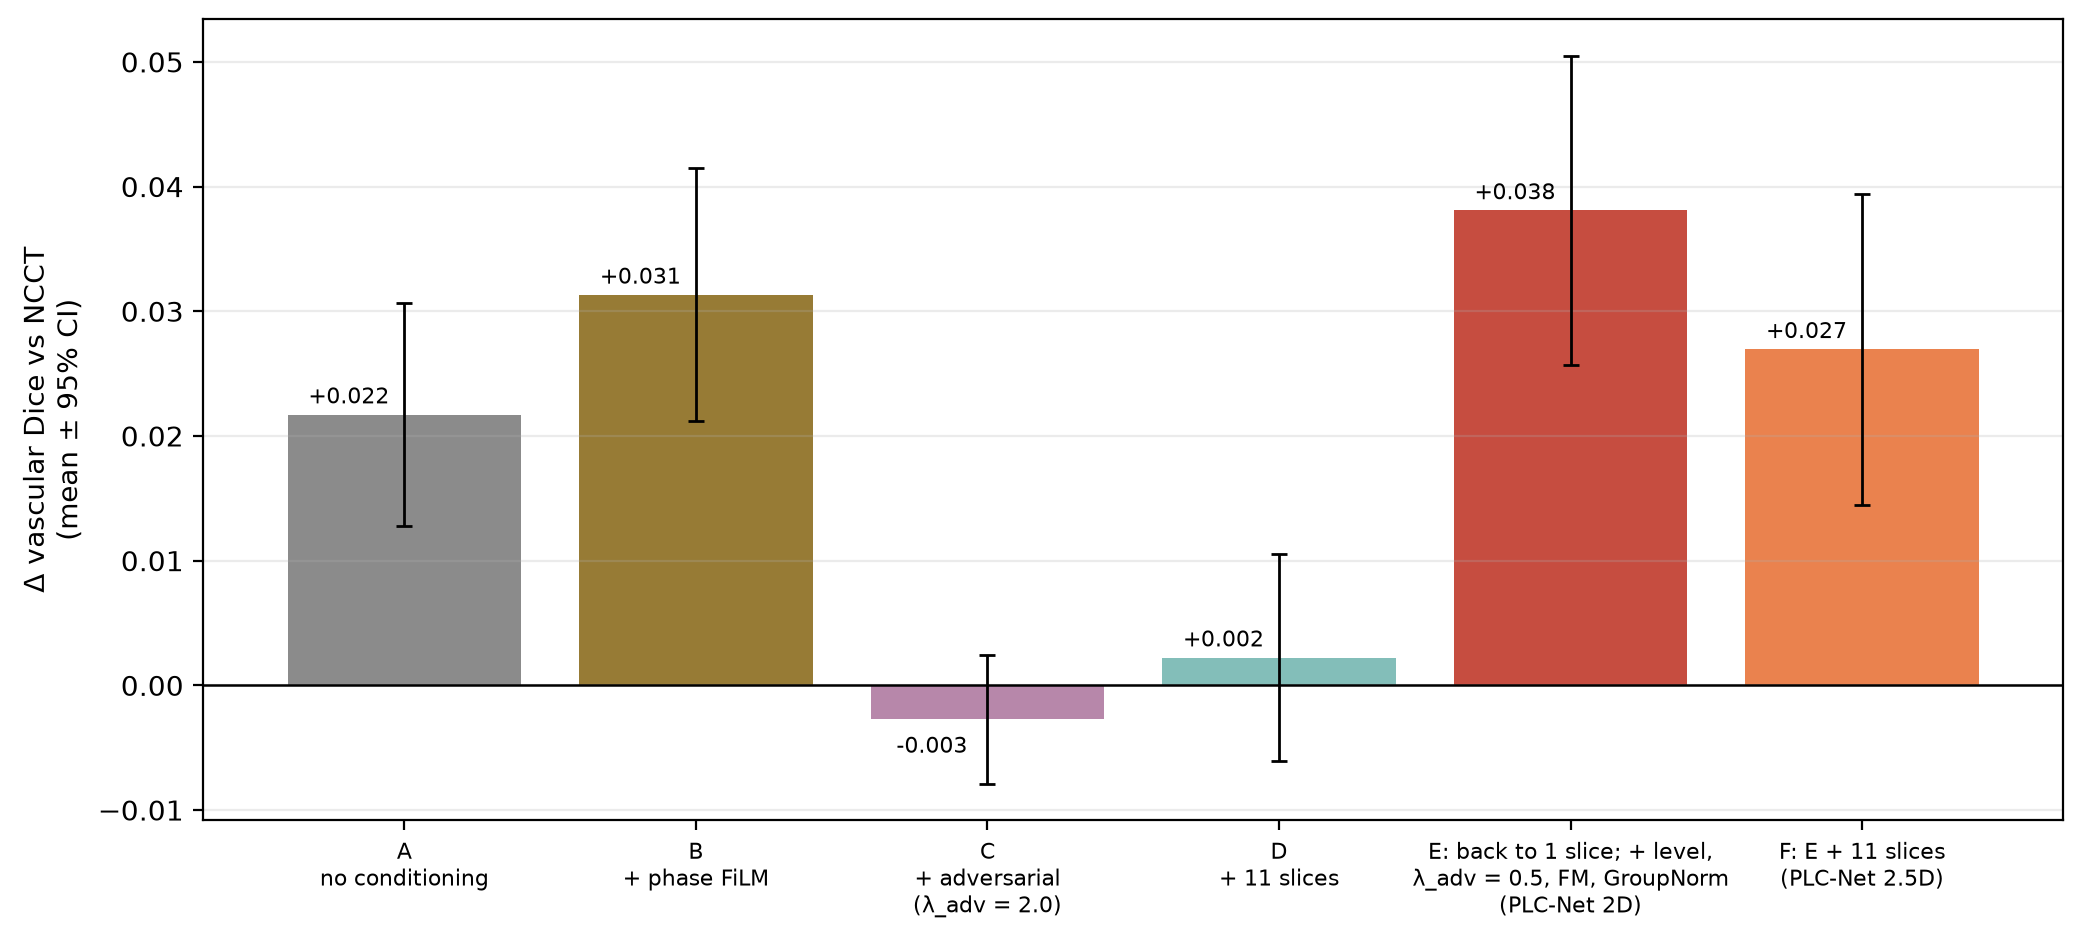
\includegraphics[width=0.95\textwidth]{synthesis/fig7_ablation_ladder.png}
\caption{اثر خالص پایین‌دستی (میانگین و فاصله‌ی اطمینان \عدد{۹۵} درصد) برای پیکربندی‌های \lr{A} تا \lr{F}؛ برای \lr{E} و \lr{F} روند آموزش هر دو، وزن‌های نماینده‌ی جدول~\ref{tab:syn-ablation} برجسته شده‌اند.}
\label{fig:syn-ladder}
\end{figure}

\subsection*{دو مبنای حذفی داخلی تک‌پویش}

جدا از زنجیره‌ی \lr{A} تا \lr{F}، که همگی چندپویشی و شرطی‌اند، دو مبنای حذفی \emph{تک‌پویش} و \emph{بدون شرط} نیز آموزش داده شدند تا سهم خودِ جمله‌ی تخاصمی و شرط‌گذاری، جدا از زیان بازسازی \lr{L1} وزن‌دار اندامی، روشن شود: \lr{L1}-اندام (بدون جمله‌ی تخاصمی) و \lr{L1} ناهم‌وردایی (وایازش ناهم‌وردایی بخش~\ref{sec:m-uncertainty}). جدول~\ref{tab:syn-l1baselines} ارقام آن‌ها را، در کنار \lr{PLC-Net} دوبعدی برای مرجع، گزارش می‌کند.

\begin{table}[H]
\centering
\footnotesize
\caption{دو مبنای حذفی تک‌پویش و بدون شرط، در برابر \lr{PLC-Net} دوبعدی، در پویش وریدی. اثر خالص پایین‌دستی برای \lr{L1} ناهم‌وردایی محاسبه نشده است، چون در ارزیابی پایین‌دستی جدول~\ref{tab:syn-gap} حضور ندارد. بهترین مقدار پررنگ و دومین مقدار بهتر زیرخط‌دار است.}
\label{tab:syn-l1baselines}
\begin{tabular}{|l|c|c|c|c|c|}
\hline
\textbf{مدل} & \lr{\textbf{featHU}}$\downarrow$ & \lr{\textbf{PSNR}}$\uparrow$ & \lr{\textbf{FID}}$\downarrow$ & \textbf{دقت پویش} & \textbf{اثر خالص پایین‌دستی} \\
\hline
\lr{L1}-اندام & \textbf{\عدد{۱۲٫۹۰}} & \underline{\عدد{۳۰٫۶۶}} & \عدد{۲۸٫۳} & \عدد{۱٫۰۰} & \textbf{\عدد{+۰٫۰۵۳۵}} \\
\hline
\lr{L1} ناهم‌وردایی & \underline{\عدد{۱۴٫۴۶}} & \textbf{\عدد{۳۰٫۸۲}} & \underline{\عدد{۲۲٫۴}} & \عدد{۱٫۰۰} & --- \\
\hline
\lr{PLC-Net} دوبعدی (مرجع) & \عدد{۱۴٫۵۵} & \عدد{۲۹٫۶۴} & \textbf{\عدد{۹٫۶}} & \عدد{۱٫۰۰} & \underline{\عدد{+۰٫۰۵۲۳}} \\
\hline
\end{tabular}
\end{table}

هر دو مبنا در \lr{featHU}، \lr{PSNR} و \lr{SSIM} از \lr{PLC-Net} کمی جلوترند، اما در \lr{FID} به‌روشنی عقب‌ترند (\عدد{۲۸٫۳} و \عدد{۲۲٫۴} در برابر \عدد{۹٫۶})؛ یعنی وفاداری تصویردانه‌ای بالاتر، اینجا با واقع‌نمایی ادراکی کمتر همراه است. \lr{L1}-اندام در اثر خالص پایین‌دستی نیز با \lr{PLC-Net} هم‌رده است (\عدد{+۰٫۰۵۳۵} در برابر \عدد{+۰٫۰۵۲۳})، اما هیچ‌یک از این دو مبنا پویش یا سطح تقویت را نمی‌پذیرد و برای هر پویش باید مدلی جداگانه آموزش ببیند؛ کنترل صریح، نه دقت پایین‌دستی، تمایز \lr{PLC-Net} با آن‌هاست.


\subsection*{مطالعه‌ی حذفی هم‌ترازسازی: سهم هر گام پیش‌پردازش}


دو گام دیگر نیز پیاده‌سازی و آزموده شدند و در مسیر نهایی نماندند. جدول~\ref{tab:reg-excluded} آن‌ها را معرفی می‌کند و نتیجه‌ی هر دو در ادامه می‌آید.

\begin{table}[H]
\centering
\footnotesize
\caption{گام‌های آزموده‌شده و کنارگذاشته‌شده از مسیر نهایی هم‌ترازسازی.}
\label{tab:reg-excluded}
\begin{tabular}{|p{3.2cm}|p{5.2cm}|p{5.2cm}|}
\hline
\textbf{گام آزموده‌شده} & \textbf{دلیل بررسی} & \textbf{تعریف} \\
\hline
هم‌ترازی درشت مرکز جرم & پیش از گذرهای صلب، یک جابه‌جایی درشت از مرکز جرم چهار اندام بزرگ برآورد و اعمال می‌شد. & گذر صفر همان تصحیح را، به‌صورت بسته و همراه با چرخش، انجام می‌دهد. \\
\hline
گذر پالایشی روی بزرگی شیو (\lr{gradient magnitude}) & گذر سومی که معیار را از شدت روشنایی به بزرگی شیو تغییر می‌داد، با این استدلال که تزریق ماده‌ی حاجب \emph{سطح} روشنایی را جابه‌جا می‌کند اما \emph{لبه}ها را در جای خود نگه می‌دارد. & همبستگی محلی روی بزرگی شیو، محدود به نقاب اندام‌ها، با دروازه‌ی پذیرش مبتنی‌بر خطای مرکز. \\
\hline
\end{tabular}
\end{table}

جدول~\ref{tab:reg-ablation} نتیجه‌ی افزودن تدریجی گام‌ها را نشان می‌دهد. بخش بالای
جدول زنجیره‌ی کامل گام‌های آزموده است و بخش پایین همان زنجیره بدون گام هم‌ترازی
درشت مرکز جرم، که مسیر پیشنهادی نهایی است.

\begin{table}[H]
\centering
\footnotesize
\caption{سهم هر گام پیش‌پردازش در دقت هم‌ترازی، روی \عدد{۵۷۷} مورد مقایسه از \عدد{۲۶} نوبت. همه‌ی ستون‌ها مقدار معمول‌اند و ستون سوم بازه‌ای است که نیمی از موارد در آن قرار دارند. برای دایس مقدار بیشتر و برای دو فاصله مقدار کمتر بهتر است. ${}^{\dagger}$خروجی «فقط برش مشترک» تنها برای \عدد{۲۳} نوبت (\عدد{۴۹۸} مورد مقایسه) موجود است. بهترین مقدار پررنگ و دومین مقدار بهتر زیرخط‌دار است.}
\label{tab:reg-ablation}
\begin{tabular}{|p{5.2cm}|c|c|c|c|}
\hline
\textbf{گام‌ها} & \textbf{دایس} & \textbf{نیمی از موارد} & \textbf{خطای مرکز (میلی‌متر)} & \textbf{فاصله‌ی مرزها (میلی‌متر)} \\
\hline
\multicolumn{5}{|l|}{\emph{زنجیره‌ی کامل گام‌های آزموده}} \\
\hline
فقط برش مشترک${}^{\dagger}$ & \عدد{۰٫۷۹۷} & \عدد{۰٫۶۲--۰٫۸۹} & \عدد{۲٫۶۲} & \عدد{۳٫۳۵} \\
\hline
\lr{+} هم‌ترازی درشت مرکز جرم & \عدد{۰٫۷۷۳} & \عدد{۰٫۵۷--۰٫۸۸} & \عدد{۲٫۸۹} & \عدد{۳٫۶۷} \\
\hline
\lr{+} هم‌ترازی صلب اولیه (کابش) & \عدد{۰٫۷۹۲} & \عدد{۰٫۶۲--۰٫۸۹} & \underline{\عدد{۲٫۲۷}} & \عدد{۳٫۳۵} \\
\hline
\lr{+} پالایش صلب (نلدر-مید) & \underline{\عدد{۰٫۸۱۶}} & \عدد{۰٫۶۳--۰٫۹۰} & \textbf{\عدد{۲٫۰۸}} & \عدد{۳٫۳۵} \\
\hline
\lr{+} گذر روی بزرگی شیو & \underline{\عدد{۰٫۸۱۶}} & \عدد{۰٫۶۳--۰٫۹۰} & \textbf{\عدد{۲٫۰۸}} & \عدد{۳٫۳۵} \\
\hline
\multicolumn{5}{|l|}{\emph{مسیر پیشنهادی: همان گام‌ها بدون هم‌ترازی درشت مرکز جرم}} \\
\hline
برش مشترک \lr{+} هم‌ترازی صلب اولیه & \عدد{۰٫۷۹۷} & \عدد{۰٫۶۳--۰٫۸۹} & \underline{\عدد{۲٫۲۷}} & \عدد{۳٫۳۵} \\
\hline
برش مشترک \lr{+} هم‌ترازی صلب اولیه \lr{+} پالایش صلب & \textbf{\عدد{۰٫۸۲۱}} & \عدد{۰٫۶۵--۰٫۹۰} & \textbf{\عدد{۲٫۰۸}} & \عدد{۳٫۳۵} \\
\hline
\end{tabular}
\end{table}

\مهم{یکم ــ هم‌ترازی درشت مرکز جرم کمکی نمی‌کند و در جایی که فعال می‌شود آسیب
می‌زند.} افزودن این گام به برش مشترک، دایس را در \عدد{۴۰} مورد بدتر و تنها در
\عدد{۱۶} مورد بهتر می‌کند ($p$ برابر \عدد{۰٫۰۰۱۸}). بررسی موارد نشان می‌دهد این
گام تنها در \عدد{۸} جفت پویش از \عدد{۴} نوبت جابه‌جایی اعمال کرده است. در سه جفت
اثر آن ناچیز بود، اما در پنج جفت دیگر خطای مرکز اندام را به‌طور محسوس افزایش داد؛
در دو مورد، مقدار معمول این خطا از حدود \عدد{۱۶} و \عدد{۲۳} میلی‌متر به حدود
\عدد{۴۰} میلی‌متر رسید و دایس این دو جفت به کمتر از \عدد{۰٫۰۷} افتاد. این الگو با
تطبیق نادرست اندام‌ها در این گام سازگار است. پس از دو گذر صلب، تفاوت دو شاخه
دیگر معنادار نیست (با این گام \عدد{۲۱۲} مورد بهتر و \عدد{۱۸۲} مورد بدتر؛ $p$
برابر \عدد{۰٫۱۴})، و مقدار معمول دایس بدون آن اندکی بالاتر است. این گام از مسیر
پیشنهادی کنار گذاشته شد.

\مهم{دوم ــ دو گذر صلب اثرهای مکمل دارند و هر یک روی گروه متفاوتی اثر می‌گذارد.}
هم‌ترازی صلب اولیه (کابش) در مجموع \عدد{۳۵۱} مورد را بهتر و \عدد{۱۷۹} مورد را بدتر
می‌کند ($p$ کمتر از \عدد{۰٫۰۰۱}) و تقریباً تمام این اثر در اندام‌های نرم است
(دایس از \عدد{۰٫۷۴۲} به \عدد{۰٫۷۸۴}؛ \عدد{۲۱۷} بهتر در برابر \عدد{۷۶} بدتر؛ $p$
کمتر از \عدد{۰٫۰۰۱})، در حالی که اثر آن بر مهره‌ها پس از تصحیح بونفرونی معنادار
نیست. پالایش صلب (نلدر-مید) برعکس عمل می‌کند: اثر آن بر مهره‌هاست (دایس از
\عدد{۰٫۸۸۳} به \عدد{۰٫۹۰۸}؛ \عدد{۹۰} بهتر در برابر \عدد{۲۴} بدتر؛ $p$ کمتر از
\عدد{۰٫۰۰۱}) و بر اندام‌های نرم اثر معناداری ندارد. تفسیر این الگو ساده است: حل
بسته‌ی کابش موقعیت درشت اندام‌های نرم بزرگ را تصحیح می‌کند، و پالایش مبتنی‌بر
دایس، انطباق دقیق ساختارهای صلب و کوچک را بهتر می‌کند.

نسخه‌ی نخست گذر صفر تنها بر لنگرهای استخوانی تکیه می‌کرد و افزودن اندام‌های نرم
پایدار، که در مسیر پیشنهادی به کار می‌رود، به‌طور یکنواخت نتیجه‌ی بهتری داد. این
سود را می‌توان به افزایش تعداد نقاط متناظر و بهبود شرطی‌شدگی مسئله‌ی \lr{SVD}
نسبت داد (بخش~\ref{sec:m-reg-rigid}).

\مهم{سوم ــ گذر روی بزرگی شیو هیچ اثری ندارد.} خروجی این گذر در همه‌ی
\عدد{۵۸۱} مورد و در همه‌ی شاخص‌ها دقیقاً با خروجی پالایش صلب یکسان است. دلیل روشن
است: دروازه‌ی پذیرش، که نتیجه‌ی یک گذر را تنها در صورت کاهش خطای مرکز اندام
می‌پذیرد، این گذر را در \عدد{۶۹۵} از \عدد{۶۹۹} مورد (\عدد{۹۹٫۴} درصد) رد کرد،
چون مقدار معمول خطای مرکز اندام پس از آن \عدد{۱۳٫۹۹} میلی‌متر در برابر \عدد{۲٫۰۹}
میلی‌متر پیش از آن بود. این یک نتیجه‌ی منفی است، اما نشان می‌دهد دروازه‌ی پذیرش
کار خود را کرده است: بدون آن، این گذر خطا را در حالت معمول حدود شش برابر می‌کرد و
این خرابی در انبوه داده پنهان می‌ماند.

گذر \lr{B}-اسپلاین جزو این زنجیره نیست و در بخش~\ref{sec:e-reg} جداگانه تعریف و ارزیابی می‌شود.

\subsection*{مطالعه‌ی حذفی هم‌ترازسازی: مقایسه‌ی توابع هدف}

جدول~\ref{tab:reg-objective} چهار تابع هدف را مقایسه می‌کند. این جدول نشان می‌دهد وقتی معیار روی نقاب اندام‌ها حساب می‌شود، کدام شکل معیار تبدیل را بهتر برآورد می‌کند. هر چهار اجرا مدل تبدیل، مقداردهی اولیه، بهینه‌ساز و خط‌کش ارزیابی یکسان دارند و فقط در تابع هدف فرق می‌کنند (طرح آزمایش در بخش~\ref{sec:e-setup-reg}). این اجراها مستقل از زنجیره‌ی جدول~\ref{tab:reg-ablation} انجام شده‌اند و مجموعه‌ی اندام‌هایشان فرق می‌کند، پس ارقامشان با آن جدول یکی نیست.

\begin{table}[H]
\centering
\footnotesize
\caption{مقایسه‌ی چهار تابع هدف برای پالایش صلب، همه روی نقاب اندام‌ها، روی \عدد{۵۷۷} مورد مقایسه. دایس و خطای مرکز اندام مقدار معمول‌اند؛ ستون آخر درصد موارد شکست (دایس کمتر از \عدد{۰٫۵}) است. بهترین مقدار پررنگ و دومین مقدار بهتر زیرخط‌دار است.}
\label{tab:reg-objective}
\begin{tabular}{|p{6.4cm}|c|c|c|}
\hline
\textbf{تابع هدف} & \textbf{دایس} & \textbf{خطای مرکز (میلی‌متر)} & \textbf{شکست (درصد)} \\
\hline
خطای مرکز اندام \lr{+} دایس (شکل تابع مسیر نهایی) & \عدد{۰٫۷۹۳} & \textbf{\عدد{۱٫۹۵}} & \underline{\عدد{۱۳٫۷}} \\
\hline
همبستگی لبه‌ها (بزرگی شیو سوبل) & \عدد{۰٫۷۶۱} & \عدد{۲٫۹۰} & \عدد{۱۸٫۲} \\
\hline
توصیفگر ساختاری \lr{MIND} & \underline{\عدد{۰٫۷۹۸}} & \عدد{۲٫۴۰} & \عدد{۱۴٫۹} \\
\hline
خطای مرکز اندام \lr{+} دایس \lr{+} همبستگی لبه‌ها & \textbf{\عدد{۰٫۸۰۵}} & \underline{\عدد{۱٫۹۷}} & \textbf{\عدد{۱۳٫۵}} \\
\hline
\end{tabular}
\end{table}

تابع همبستگی لبه‌ها ضعیف‌ترین نتیجه را دارد. در برابر تابع ترکیبی (ردیف آخر)، این تابع در \عدد{۱۴۲} مورد بهتر و در \عدد{۳۹۸} مورد بدتر است ($p$ کمتر از \عدد{۰٫۰۰۱})؛ خطای مرکز اندام آن \عدد{۴۷} درصد بیشتر است و نرخ شکستش \عدد{۱۸٫۲} درصد در برابر \عدد{۱۳٫۵} درصد است.

تفاوت در همه‌ی گروه‌ها یکسان نیست. در مقایسه‌ی تابع ترکیبی با تابع لبه، دایس اندام‌های نرم از \عدد{۰٫۷۵۵} به \عدد{۰٫۸۲۱} می‌رسد (\عدد{۲۵۵} بهتر در برابر \عدد{۵۱} بدتر) و دایس رگ‌های بزرگ از \عدد{۰٫۶۳۷} به \عدد{۰٫۶۸۶} (\عدد{۷۹} در برابر \عدد{۳۱}). هر دو معنادارند ($p$ کمتر از \عدد{۰٫۰۰۱}). در مهره‌ها تفاوتی دیده نمی‌شود (\عدد{۰٫۸۸۸} و \عدد{۰٫۸۹۱}؛ \عدد{۶۴} در برابر \عدد{۶۰}). همین الگو در مقایسه‌ی «خطای مرکز اندام \lr{+} دایس» با تابع لبه هم تکرار می‌شود.

افزودن جمله‌ی لبه به «خطای مرکز اندام \lr{+} دایس» در هیچ گروهی تفاوت معناداری نمی‌دهد (در مجموع \عدد{۲۶۱} بهتر در برابر \عدد{۲۴۹} بدتر؛ $p$ برابر \عدد{۰٫۶۳}). به همین دلیل مسیر نهایی همان تابع ساده‌تر رابطه‌ی~\ref{eq:pass1-loss} را به کار می‌گیرد.

\lr{MIND} از این تابع ساده ضعیف‌تر است (\عدد{۲۱۷} بهتر در برابر \عدد{۳۲۴} بدتر؛ $p$ کمتر از \عدد{۰٫۰۰۱}). با این حال دایس معمول \lr{MIND} (\عدد{۰٫۷۹۸}) کمی بالاتر از تابع ساده (\عدد{۰٫۷۹۳}) است. برتری تابع ساده در خطای مرکز (\عدد{۱٫۹۵} در برابر \عدد{۲٫۴۰} میلی‌متر)، نرخ شکست (\عدد{۱۳٫۷} در برابر \عدد{۱۴٫۹} درصد) و مقایسه‌ی مورد به مورد است، نه در دایس معمول.

یک توضیح ممکن برای ضعف تابع لبه این است که لبه‌ی درون اندام‌های نرم و رگ‌ها ضعیف است و با تباین تغییر می‌کند، در حالی که لبه‌ی قشری مهره‌ها در همه‌ی پویش‌ها تیز است. این با الگوی بالا می‌خواند، ولی آن را جداگانه نیازموده‌ایم. توضیح دیگر فرسایش \عدد{۴} میلی‌متری است که نقاط را از مرز اندام دور می‌کند و فقط گرادیان درونی را برای مقایسه می‌گذارد. گذر بزرگی شیو (جدول~\ref{tab:reg-excluded}) هم، که دروازه‌ی پذیرش \عدد{۹۹٫۴} درصد آن را رد کرد، با ضعف معیار لبه در این داده هم‌سو است.

این نتیجه سه حد دارد.
\begin{itemize}
\item این جدول \emph{نوع معیار} را روی دامنه‌ی ثابتِ نقاب مقایسه می‌کند. درباره‌ی «کل تصویر در برابر نقاب» چیزی نمی‌گوید.
\item \lr{MIND} فقط در پالایش صلب و بدون جمله‌ی آناتومیک آزموده شد. بهترین دقت کل این مطالعه از \lr{DEEDS} آمد که خودش بر توصیفگر \lr{MIND} بنا شده است؛ اما \lr{DEEDS} در چند چیز هم‌زمان با مسیر ما فرق دارد (غیرصلب، کل تصویر، بهینه‌سازی گسسته)، پس مقایسه‌ی آن‌ها اثر \lr{MIND} را جدا نمی‌کند.
\item واحد آزمون، ردیف‌های اندام\lr{×}جفت‌اند و از \عدد{۲۶} بیمار می‌آیند. اندام‌های یک جفت مستقل نیستند، پس مقدار $p$ خوش‌بینانه است.
\end{itemize}

\section{تحلیل حساسیت و تحلیل‌های تکمیلی}
\label{sec:e-analysis}

این بخش نتیجه‌ی اصلی را از چند زاویه می‌آزماید: درستی کنترل پویش و سطح، هم‌راستایی معیارهای تصویری با سودمندی پایین‌دستی، حساسیت نتیجه به انتخاب معیار پایین‌دستی، و علت شکست کیسه‌ی صفرا.


\subsection*{اثر استانداردسازی سطح بر ارزیابی شرط پویش}

حالت ساده‌ی «جمعیتی» (یعنی یک بردار شرط تماماً صفر) برای مدل \emph{چندپویشی} بد-تعریف است و این نکته به‌سادگی از چشم پنهان می‌ماند. استانداردسازِ سطح، آمار هر دو پویش را با هم میانگین می‌گیرد؛ در نتیجه $z=0$ سطحی را درخواست می‌کند که به \emph{هیچ‌یک} از دو پویش تعلق ندارد؛ مقداری میان میانگین وریدی و میانگین شریانی.

پیامد این خطا وارونه‌کننده است: تحت این حالت، معیار دقت پویش مدلی را که به شرط خود \emph{وفادار} است جریمه می‌کند و مدلی را که آن را \emph{نادیده} می‌گیرد پاداش می‌دهد. این نکته پس از تولید جدول‌های مقایسه‌ای شناسایی شد. جدول‌های اصلی در همان حالت \lr{population} نگه داشته شده‌اند تا همه‌ی بازوها، از جمله پیکربندی‌های بدون ورودی سطح، با یک قرارداد امتیاز گرفته باشند؛ به همین دلیل ارقام دقت پویش و \lr{featHU} این جدول‌ها برای مدلی که به بردار سطح وفادار است (پیکربندی \lr{F}) کران پایین‌اند، نه برآورد توان مدل. ارزیابی مجدد با حالت \lr{population\_phase} در زیربخش بعد جداگانه گزارش می‌شود.

حالت \lr{population\_phase} میانگین آموزشیِ \emph{مخصوص همان پویش} را می‌دهد؛ برای آئورت، \عدد{۱۳۳٫۹} واحد هانسفیلد در پویش وریدی و \عدد{۲۸۱٫۷} در پویش شریانی، در برابر میانگین تجمیعی \عدد{۲۰۷٫۴}.

اما این اصلاح را نباید بیش از آن‌چه هست جلوه داد: \lr{population\_phase} یک حالت \emph{استنتاج} است و تنها پیش‌فرض \emph{ارزیابی} را اصلاح می‌کند. درهم‌تنیدگی دو علامت شرط در زمان \emph{آموزش} رخ می‌دهد، چون بردارهای سطح با همان متعارف‌سازی تجمیعی ساخته می‌شوند. رفع ریشه‌ای آن نیازمند متعارف‌سازی درون‌پویشی و بازآموزی است و کار آتی محسوب می‌شود.

\subsection*{کنترل پویش}

هر مدل شرطی دو بار استنتاج شد، یک‌بار با شرط وریدی و یک‌بار با شرط شریانی، و هر دو خروجی در برابر همان مرجع وریدی سنجیده شدند. اگر شرط‌گذاری کار کند، خروجی با شرط وریدی باید دایس عروقی بالاتری بگیرد.

هفت اجرا از هشت اجرای شرطی با شرط وریدی دایس عروقی به‌طور معنادار بالاتری دارند: تفاوت میان \عدد{+۰٫۰۰۸} و \عدد{+۰٫۰۳۷}، همگی با $p < 0.0001$، و بالاتر در \عدد{۱۸} تا \عدد{۲۰} مورد (یکی از اجراها \عدد{۱۹} مورد زوجی دارد). برای \lr{PLC-Net} دوبعدی تفاوت \عدد{+۰٫۰۳۵۳} است ($p < 0.0001$، بالاتر در هر \عدد{۲۰} مورد). شکل~\ref{fig:syn-phase} این پاسخ‌ها را نشان می‌دهد.

مدل بدون شرط (پیکربندی \lr{A}) ورودی پویش ندارد؛ بنابراین تفاوت دو استنتاج آن تنها نوفه‌ی زنجیره‌ی ارزیابی را نشان می‌دهد، که عملاً صفر است (\عدد{−۰٫۰۰۰۰}، $p = 0.86$، بالاتر در \عدد{۹} مورد). پاسخ مدل‌های شرطی به‌روشنی بالاتر از این کف است.

تنها اجرای شرطی بدون پاسخ، پیکربندی \lr{F} در دوره‌ی \عدد{۵۳} است (\عدد{−۰٫۰۰۱۰}، $p = 0.57$، بالاتر در \عدد{۸} مورد). دسته‌بند مستقل پویش نیز به همین اجرا دقت \عدد{۰٫۲۵} می‌دهد؛ دو سنجه‌ی مستقل برای این اجرا هم‌جهت‌اند. همان پیکربندی \lr{F}، وقتی با بردار سطحِ میانگین جمعیتی مخصوص هر پویش استنتاج می‌شود، پاسخ پویش عادی دارد (\عدد{+۰٫۰۳۵۳}، بالاتر در هر \عدد{۲۰} مورد، دقت پویش \عدد{۱٫۰۰})، و وزن‌های دوره‌ی \عدد{۲۳} نیز با همان نوع استنتاج به دقت پویش \عدد{۱٫۰۰} و \lr{featHU} برابر \عدد{۱۶٫۸} می‌رسند، در برابر \عدد{۰٫۷۵} و \عدد{۲۲٫۰} در جدول~\ref{tab:syn-fidelity}. بنابراین پاسخ پویش پیکربندی \lr{F} به بردار سطحی که هنگام استنتاج داده می‌شود وابسته است و نه به وزن‌های مدل؛ زیربخش سازوکار به این نکته بازمی‌گردد.

\begin{figure}[H]
\centering
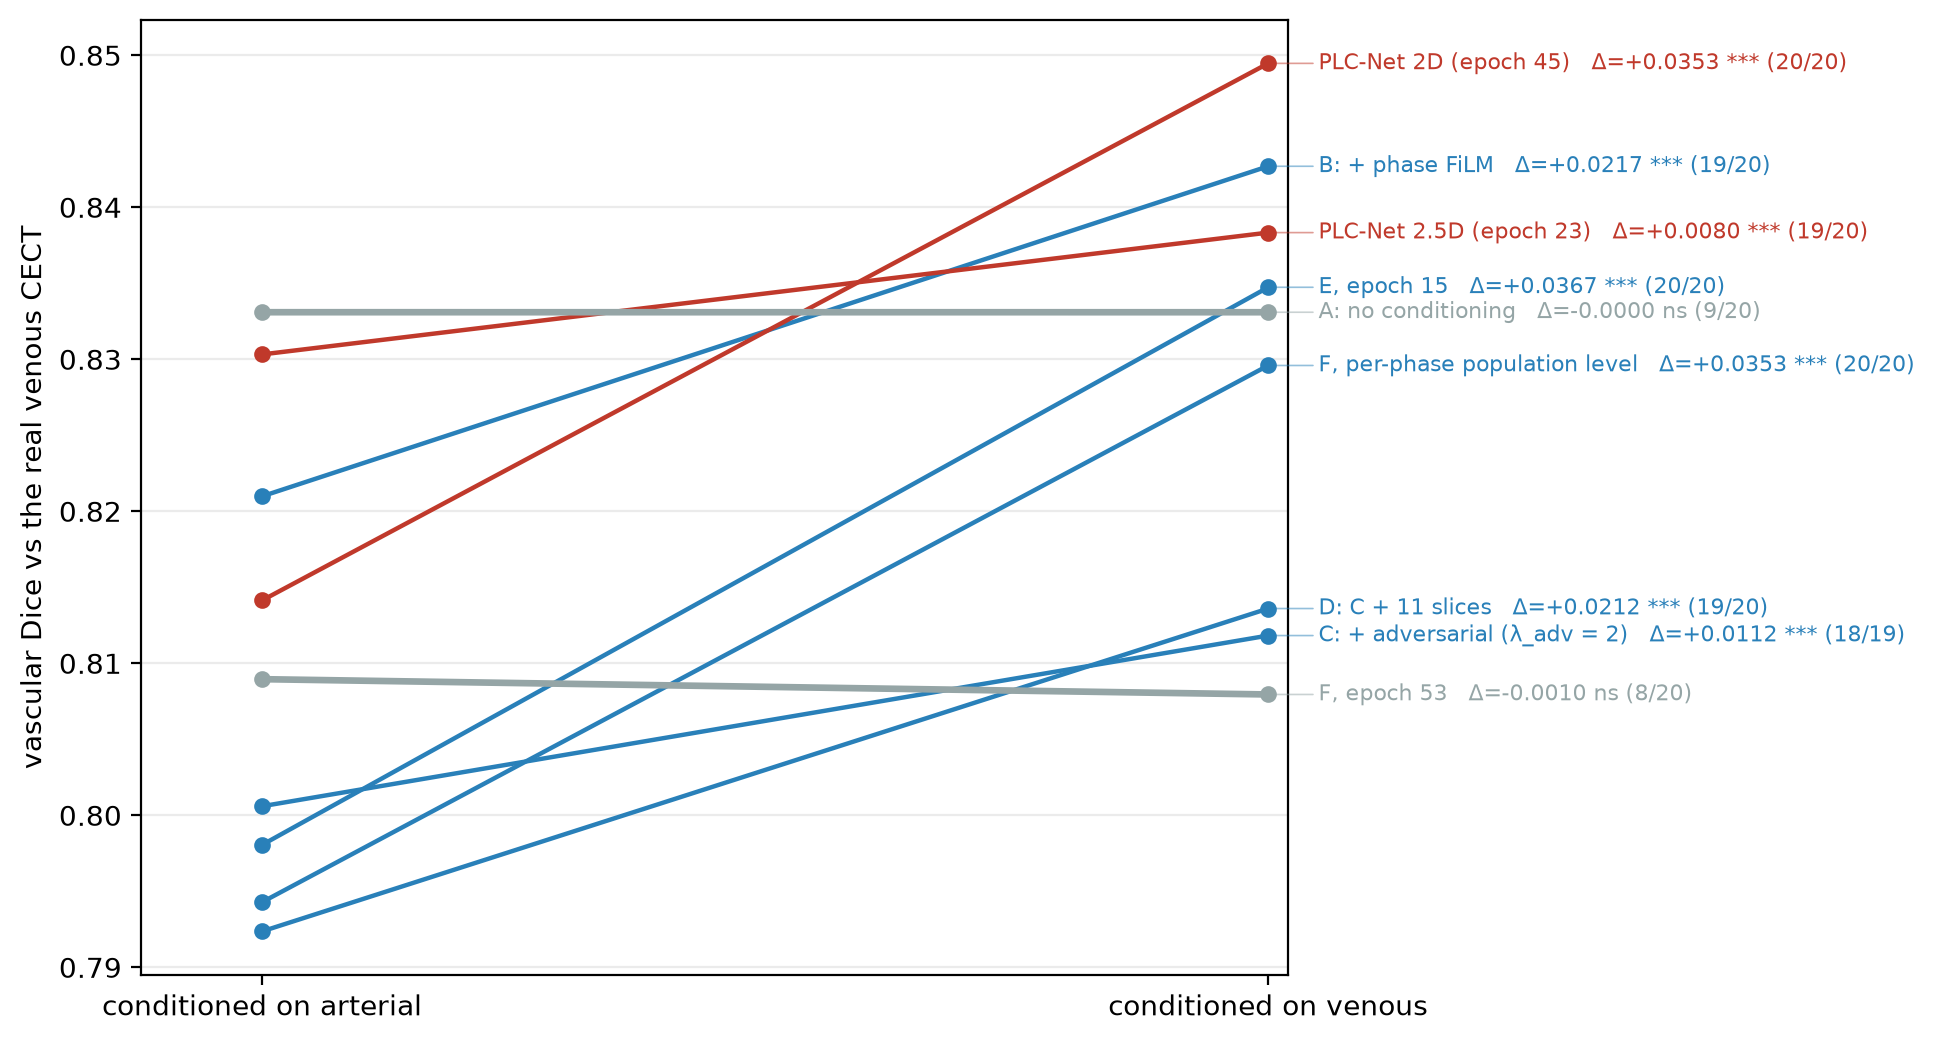
\includegraphics[width=0.9\textwidth]{synthesis/fig2_phase_sensitivity.png}
\caption{دایس عروقی هر مدل شرطی، یک‌بار با شرط شریانی و یک‌بار با شرط وریدی، هر دو در برابر همان مرجع وریدی. خط‌های خاکستری تفاوت معناداری ندارند: مدل بدون شرط (پیکربندی \lr{A}، نوفه‌ی زنجیره‌ی ارزیابی) و پیکربندی \lr{F} در دوره‌ی \عدد{۵۳}.}
\label{fig:syn-phase}
\end{figure}

شکل~\ref{fig:syn-phase-img} همین تفاوت را در تصویر نشان می‌دهد: همان بیمار نمونه، یک‌بار با شرط وریدی و یک‌بار با شرط شریانی. خروجی \lr{PLC-Net} دوبعدی با شرط شریانی الگوی پویش شریانی را دارد: آئورت و حفره‌های قلب به‌روشنی از خروجی وریدی همان مدل روشن‌ترند. این خروجی از تصویر شریانی واقعی همین بیمار نیز روشن‌تر است (قرمز در ردیف تفاوت)، که با طراحی استنتاج سازگار است: سطح تقویت از میانگین جمعیتی پویش شریانی گرفته می‌شود و سطح مخصوص این بیمار قابل پیش‌بینی نیست (بخش~\ref{sec:m-syn}). خروجی شریانی \lr{PLC-Net} \عدد{۲٫۵}~بعدی تفاوت کمتری با خروجی وریدی خودش دارد، که با امضای پویش ضعیف‌تر آن در زیربخش کنترل سطح سازگار است. مدل‌های تک‌پویش تنها یک خروجی دارند؛ در ردیف شریانی همان خروجی وریدی آن‌ها در برابر تصویر شریانی واقعی نمایش داده شده و ردیف تفاوت، کم‌تقویتی آئورت و قلب را نشان می‌دهد.

\begin{figure}[H]
\centering
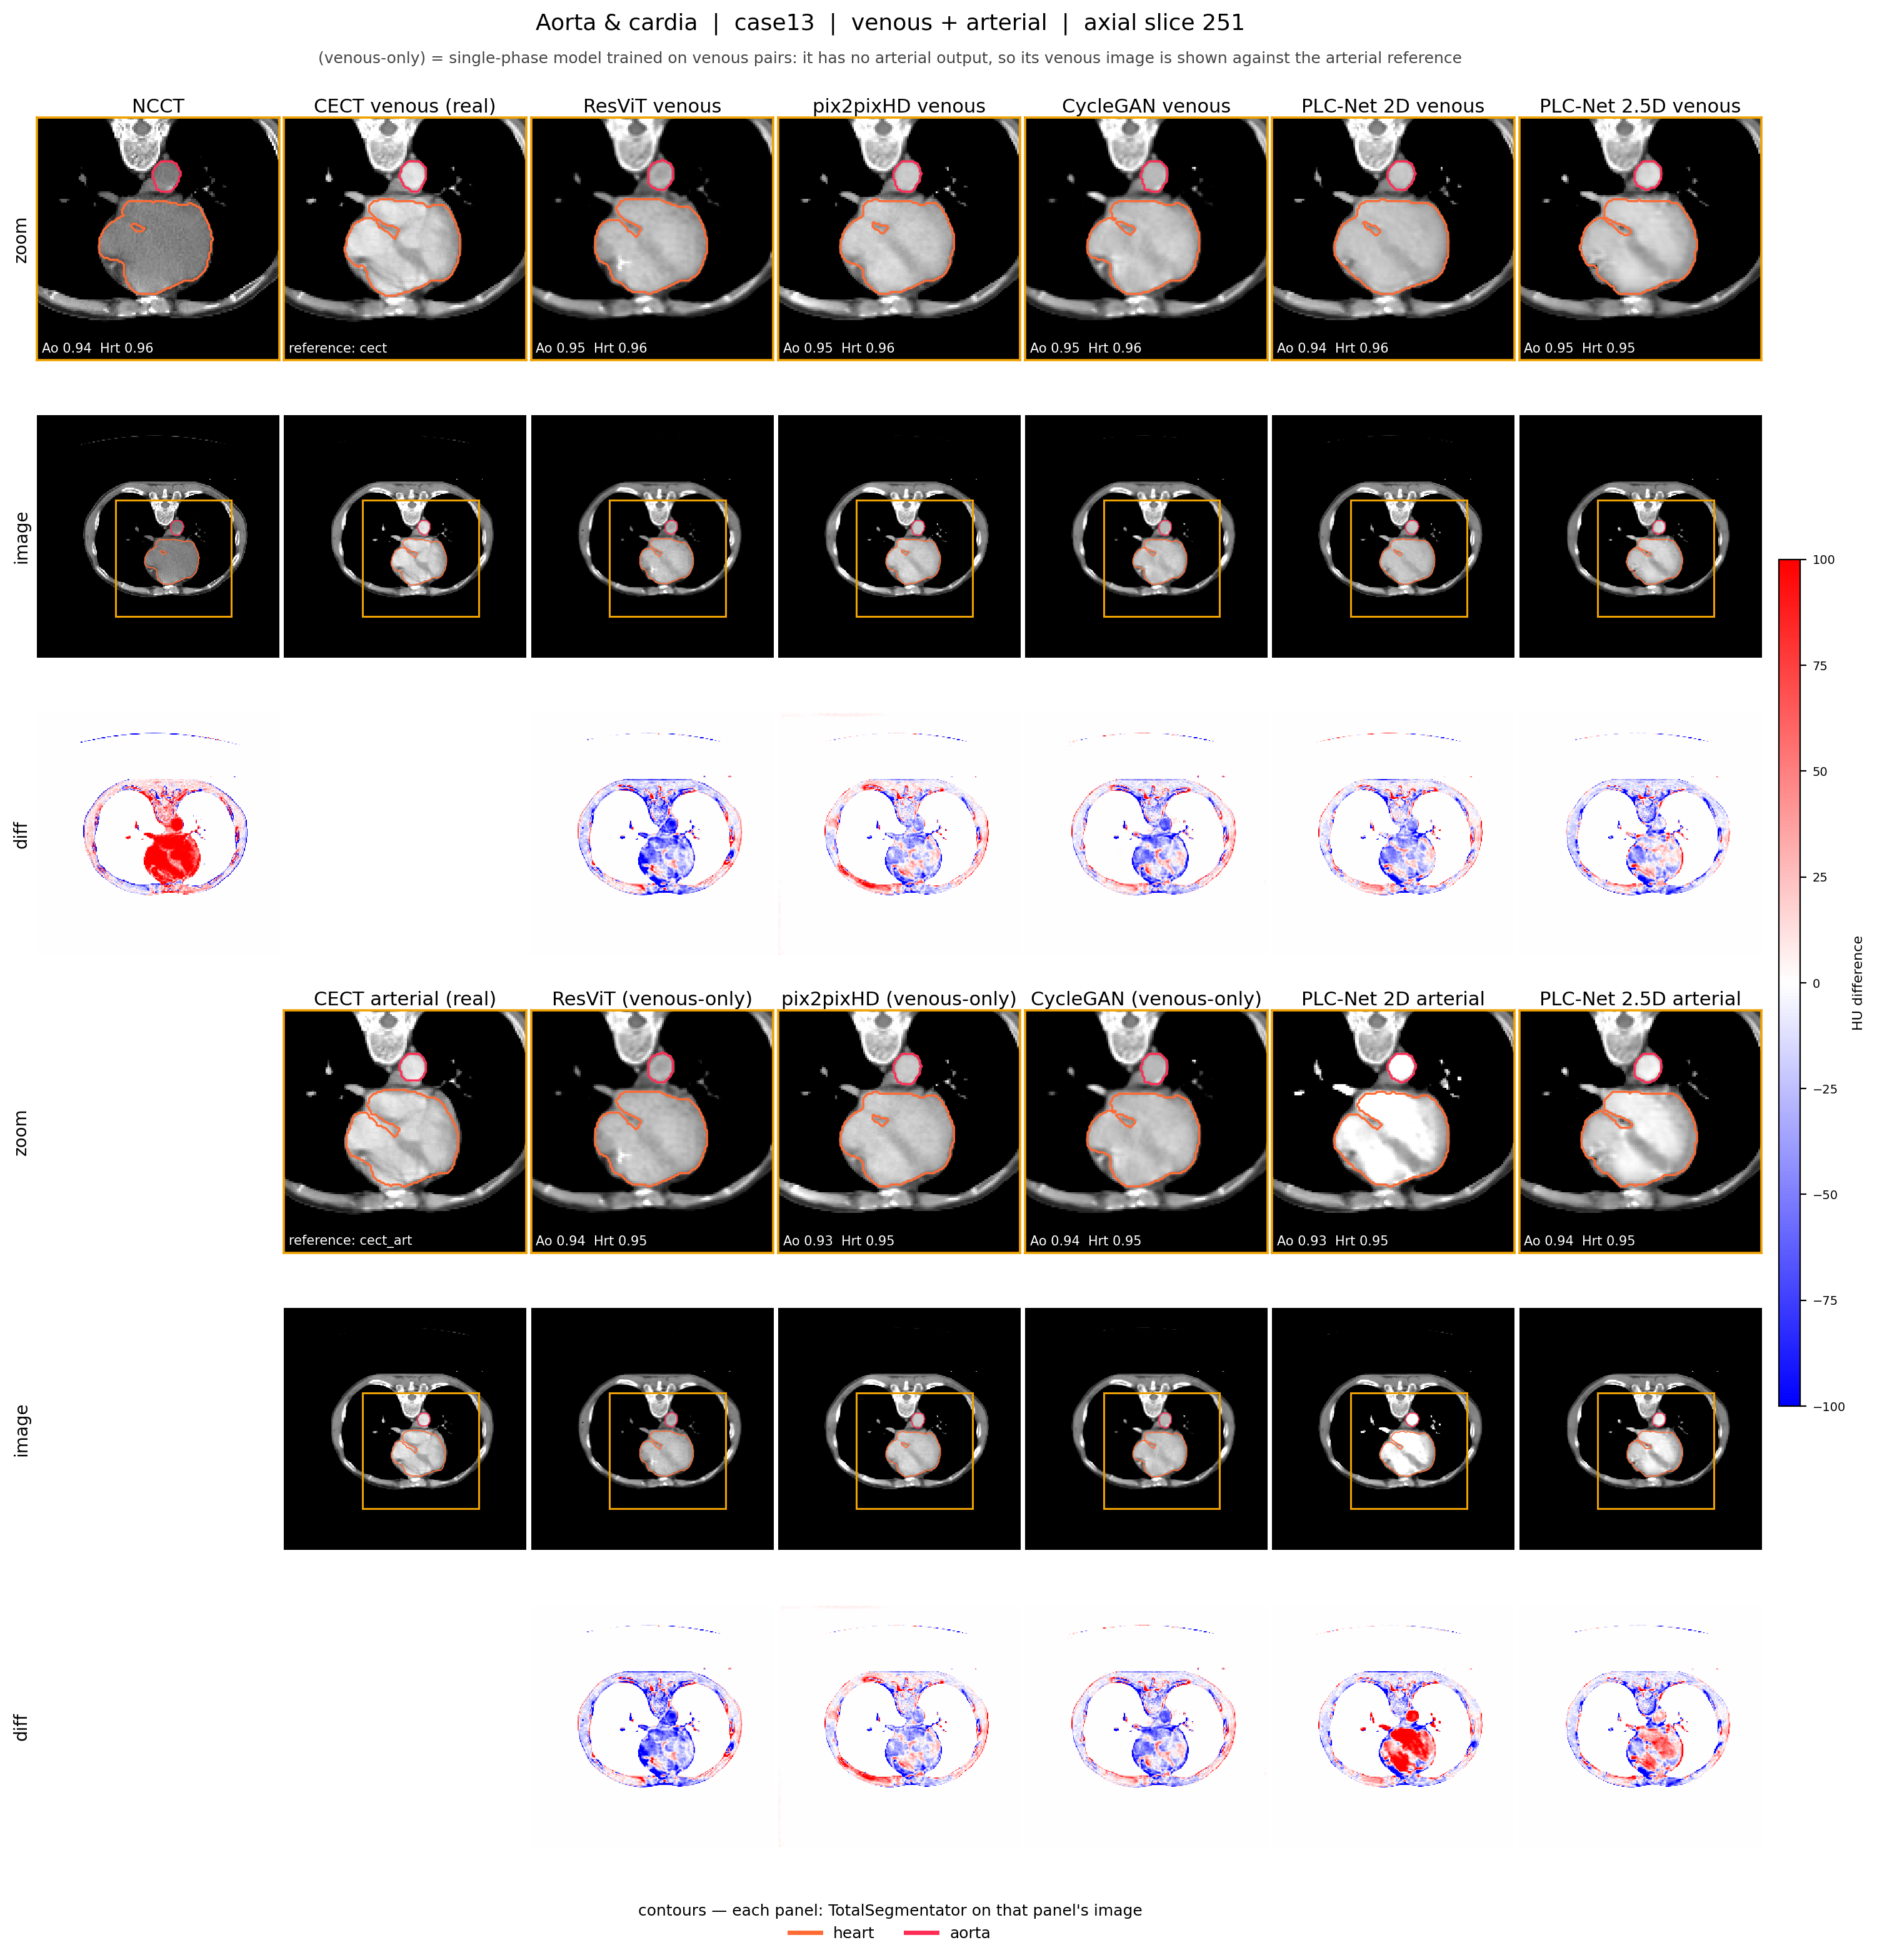
\includegraphics[width=\textwidth]{synthesis/qual_phase_case13.png}
\caption{کنترل پویش در تصویر، برای همان مورد نمونه‌ی شکل~\ref{fig:syn-cmp}، در تراز آئورت و قلب. ردیف بالا: شرط وریدی و تصویر وریدی واقعی؛ ردیف پایین: شرط شریانی و تصویر شریانی واقعی. ستون‌های «\lr{venous-only}» مدل‌های تک‌پویش‌اند که خروجی شریانی ندارند و خروجی وریدی آن‌ها در برابر مرجع شریانی نمایش داده شده است. پنجره، خطوط بخش‌بندی، اعداد دایس و ردیف تفاوت مانند شکل~\ref{fig:syn-cmp}؛ مرجع ردیف پایین، بخش‌بندی تصویر شریانی واقعی است.}
\label{fig:syn-phase-img}
\end{figure}

\textbf{بخش‌بندی در برابر مرجع شریانی.} خروجی‌های با شرط شریانی در برابر بخش‌بندی تصویر شریانی واقعی نیز ارزیابی شدند. بخش‌بندی مستقیم \lr{NCCT} در برابر این مرجع، در گروه عروقی دایس \عدد{۰٫۸۰۹} و در آئورت \عدد{۰٫۹۲۲} دارد. خروجی شریانی \lr{PLC-Net} دوبعدی دایس گروه عروقی را \عدد{+۰٫۰۱۴۵} ($p = 0.011$، بالاتر در \عدد{۱۴} مورد از \عدد{۲۰}) و دایس آئورت را \عدد{+۰٫۰۱۲} ($p = 0.002$، \عدد{۱۶} مورد) افزایش می‌دهد و مانند پویش وریدی روی گروه اسکلتی دایس از دست می‌دهد (\عدد{−۰٫۰۱۷}). اما این مقایسه میان پیکربندی‌ها تمایز نمی‌گذارد: مدل بدون شرط (پیکربندی \lr{A}) روی گروه عروقی \عدد{+۰٫۰۱۸۵} و پیکربندی \lr{B} \عدد{+۰٫۰۱۶۷} می‌گیرند، و تغییر ورید باب در هیچ بازویی معنادار نیست. بنابراین در پویش شریانی سود پایین‌دستی از جنس بهبود عمومی مرز عروق بزرگ است و شاهد کنترل پویش، همان پاسخ درون‌مدلی شکل~\ref{fig:syn-phase} و دسته‌بند پویش است و نه دایس شریانی.

\subsection*{کنترل سطح}

دلیل وجود شرط سطح، یعنی پیش‌بینی‌ناپذیری سطح تقویت هر بیمار از روی تصویر بدون‌تزریق (بخش~\ref{sec:m-syn})، با یک کاوند خطی سنجیده شد. پیش‌بینی عدد هانسفیلد آئورت در تصویر با ماده‌ی حاجب از روی میانه‌های \lr{HU} اندام‌ها در تصویر بدون‌تزریق، با یک وایازش خطی ریج، روی داده‌ی کنارگذاشته به $R^2 = -0.105$ می‌رسد؛ یعنی بدتر از پیش‌بینی با میانگین. این کاوند تنها پیش‌بینی‌پذیری \emph{خطی} را رد می‌کند و نه هر پیش‌بین ممکن را، اما برای موجه‌کردن دریافت سطح به‌عنوان ورودی کافی است.

حالت \lr{oracle} (بخش~\ref{sec:m-syn-modes}) در ارزیابی پایین‌دستی تنها برای یک مدل
تک‌پویش سطح‌شرطیِ پیشین اجرا شده است و اثر خالص آن (\عدد{+۰٫۰۳۰}) از \lr{PLC-Net}
کمتر است؛ بنابراین آن عدد سقفی برای \lr{PLC-Net} نیست.

برای سنجش کنترل سطح، مقدار $z$ در هفت مقدار از \عدد{−۱٫۵} تا \عدد{+۱٫۵} انحراف معیار درخواست و میانه‌ی \lr{HU} هر اندام در خروجی اندازه‌گیری شد. شیب‌های خام میانه (تغییر \lr{HU} در هر واحد $z$ تقسیم بر انحراف معیار تجمیعی) چنین‌اند: پیکربندی \lr{E} در دوره‌ی \عدد{۴۵} (وزن‌های \lr{PLC-Net} دوبعدی)، \عدد{۰٫۲۹} با شرط وریدی و \عدد{۰٫۰۹} با شرط شریانی؛ پیکربندی \lr{F} در دوره‌های \عدد{۲۳} و \عدد{۵۳}، میان \عدد{۰٫۶۷} و \عدد{۰٫۸۴}.

خواندن این شیب‌ها به‌صورت خام گمراه‌کننده است. متعارف‌سازی سطح، هر اندام را روی هر دو پویش با هم استاندارد می‌کند: برای آئورت، انحراف معیار تجمیعی \عدد{۱۰۵٫۳} واحد هانسفیلد است، در حالی که انحراف معیار درون پویش وریدی در داده‌ی آموزش \عدد{۲۱٫۴} و درون پویش شریانی \عدد{۱۰۴٫۶} است. مدلی که با شرط وریدی درون توزیع وریدی بماند، برای آئورت حداکثر شیب معنادار $21.4/105.3 \approx 0.20$ دارد و شیب \عدد{۱٫۰} به معنای پیمودن دامنه‌ی پویش شریانی است. جدول~\ref{tab:syn-calib} شیب هر اندام را بر سقف درون‌پویشیِ همان اندام و همان پویش تقسیم می‌کند؛ در این مقیاس، \عدد{۱٫۰} یعنی دستگیره دقیقاً پهنای طبیعی پویش خودش را می‌پیماید.

\begin{table}[H]
\centering
\footnotesize
\caption{شیب واسنجی سطح، بهنجارشده نسبت به سقف درون‌پویشی (میانه روی هشت اندام بردار سطح). مقدار بیش از یک یعنی پاسخ مدل از دامنه‌ی طبیعی پویش درخواست‌شده فراتر رفته است. جاروب پیکربندی \lr{E} روی همان وزن‌های دوره‌ی \عدد{۴۵} انجام شده که \lr{PLC-Net} دوبعدی را تعریف می‌کنند؛ جاروب \lr{F} روی هر دو دوره‌ی گزارش‌شده.}
\label{tab:syn-calib}
\begin{tabular}{|p{3.9cm}|c|c|c|p{3.4cm}|}
\hline
\textbf{پیکربندی (دوره)} & \textbf{وریدی، میانه} & \textbf{وریدی، آئورت} & \textbf{شریانی، میانه} & \textbf{تفسیر} \\
\hline
\lr{E} دوبعدی (\عدد{۴۵})؛ \lr{PLC-Net} دوبعدی & \عدد{۰٫۶۳} & \عدد{۰٫۸۸} & \عدد{۰٫۱۰} & وریدی تا حدی کنترل‌پذیر؛ شریانی کنترل‌ناپذیر \\
\hline
\lr{F} \عدد{۲٫۵}~بعدی (\عدد{۲۳})؛ \lr{PLC-Net} \عدد{۲٫۵}~بعدی & \عدد{۱٫۰۴} & \textbf{\عدد{۳٫۶۶}} & \عدد{۰٫۸۴} & آئورت فراتر از دامنه‌ی وریدی \\
\hline
\lr{F} \عدد{۲٫۵}~بعدی (\عدد{۵۳}) & \عدد{۱٫۲۵} & \textbf{\عدد{۴٫۹۶}} & \عدد{۰٫۸۷} & آئورت فراتر از دامنه‌ی وریدی \\
\hline
\end{tabular}
\end{table}

میانه‌ی نزدیک به یکِ پیکربندی \lr{F} (\عدد{۱٫۰۴}) پراکندگی میان اندام‌ها را پنهان می‌کند: پاسخ آئورت با شرط وریدی \عدد{۳٫۷} برابر (دوره‌ی \عدد{۲۳}) و \عدد{۵٫۰} برابر (دوره‌ی \عدد{۵۳}) پهنای طبیعی پویش وریدی است. در دوره‌ی \عدد{۵۳}، جاروب $z$ آئورتِ خروجی با شرط وریدی را از \عدد{۷۹} به \عدد{۳۸۰} واحد هانسفیلد می‌برد، یعنی از مقادیر وریدی به مقادیر شریانی، در حالی که شرط پویش همچنان وریدی است. در این پیکربندی، $z$ الگوی بین‌اندامیِ تعریف‌کننده‌ی پویش را تغییر می‌دهد و نه سطح تقویت درون یک پویش.

سه اندازه‌گیری دیگر همین ترتیب را نشان می‌دهند. \textbf{امضای پویش}، یعنی اختلاف \lr{HU} آئورت و ورید باب در $z = 0$، برای پیکربندی \lr{E} با شرط شریانی \عدد{۱۹۵} و با شرط وریدی \عدد{۲۶} واحد است (فاصله‌ی \عدد{۱۶۹} واحد میان دو پویش، سازگار با فیزیولوژی)؛ برای \lr{F} در دوره‌ی \عدد{۲۳} این دو مقدار \عدد{۱۰۹} و \عدد{۷۹} (فاصله‌ی \عدد{۳۰}) و در دوره‌ی \عدد{۵۳}، \عدد{۱۱۵} و \عدد{۹۸} (فاصله‌ی \عدد{۱۷}) است. \textbf{دقت دسته‌بند پویش} در حالت سطح \lr{population} برای \lr{PLC-Net} دوبعدی، \lr{F} در دوره‌ی \عدد{۲۳} و \lr{F} در دوره‌ی \عدد{۵۳} به‌ترتیب \عدد{۱٫۰۰}، \عدد{۰٫۷۵} و \عدد{۰٫۲۵} است (و برای هر دو اجرای \lr{F} در حالت \lr{population\_phase} برابر \عدد{۱٫۰۰}؛ پیکربندی \lr{E} در این حالت استنتاج نشده است)، و \textbf{پاسخ پویش پایین‌دستی} \عدد{+۰٫۰۳۵۳}، \عدد{+۰٫۰۰۸۰} و \عدد{−۰٫۰۰۱۰}. وزن‌های دوره‌ی \عدد{۱۵} همان پیکربندی \lr{E} (چک‌پوینت اعتبارسنجی) نیز دقت پویش \عدد{۱٫۰۰} و پاسخ \عدد{+۰٫۰۳۶۷} دارند.

پیکربندی دوبعدی \lr{E} تنها پیکربندی‌ای است که هر دو علامت را هم‌زمان حفظ می‌کند: پاسخ پویش کامل، و دستگیره‌ی سطحی که \عدد{۶۳} درصد دامنه‌ی درون‌پویشی وریدی را می‌پیماید (\عدد{۸۸} درصد برای آئورت). در میان پیکربندی‌های شرطی، بیشترین اثر خالص پایین‌دستی نیز به همین پیکربندی تعلق دارد. پاسخ به سطح \emph{شریانی} در این پیکربندی نزدیک صفر است: شیب بهنجارشده در همه‌ی اندام‌ها حدود \عدد{۰٫۱۰} است ($r^2$ از \عدد{۰٫۰۴} تا \عدد{۰٫۹۵}).

\subsection*{سازوکار: درهم‌تنیدگی دو علامت شرط}

بردار شرط سطح خود تا حد زیادی پویش را مشخص می‌کند. با دسته‌بندی پویش \emph{تنها} از روی بردارهای استانداردشده‌ی هشت‌اندامی سطح در داده‌ی آموزش، تحلیل تفکیکی خطی با اعتبارسنجی یکی-بیرون به دقت \عدد{۰٫۹۴۲} می‌رسد ($n = 155$ بردار، مواردی که هر هشت اندام را دارند). این اطلاعات در الگوی میان اندام‌هاست و نه در یک جابه‌جایی سراسری: آئورت و قلب در پویش شریانی بالاترند (دقت تک‌اندام \عدد{۰٫۸۸} و \عدد{۰٫۸۷}) و کبد، ورید اجوف تحتانی و ورید باب در پویش وریدی (\عدد{۰٫۹۱}، \عدد{۰٫۸۱} و \عدد{۰٫۷۴}).

بنابراین شبکه دو ورودی دریافت می‌کند که یکی دیگری را با دقت حدود \عدد{۹۴} درصد پیش‌بینی می‌کند، و هیچ جمله‌ای در تابع هدف استفاده از هر دو را الزامی نمی‌کند. در عمل دو نسخه به دو سوی مخالف رفته‌اند: مدل دوبعدی به شناسه‌ی پویش پاسخ قوی و به سطح پاسخ محدود می‌دهد، و مدل \عدد{۲٫۵}~بعدی به سطح پاسخی فراتر از دامنه‌ی طبیعی و به شناسه‌ی پویش پاسخ ضعیف. مشاهده‌ی زیربخش کنترل پویش با این تصویر سازگار است: وقتی بردار سطحِ مخصوص پویش درخواستی به مدل \عدد{۲٫۵}~بعدی داده می‌شود، پویش درست تولید می‌شود، یعنی اطلاعات پویش عمدتاً از مسیر بردار سطح به این مدل می‌رسد. خودِ این جدایی رفتار اندازه‌گیری شده است؛ این‌که متعارف‌سازی تجمیعی بردار سطح در زمان آموزش علت آن باشد، تفسیری است که با بازآموزی آزموده نشده است.

\subsection*{اعتبار معیارهای تصویری}

در میان \عدد{۲۰} بازوی وریدی، هم‌بستگی اسپیرمن هر معیار تصویری با اثر خالص پایین‌دستی محاسبه شد. معیارها چنان جهت داده شده‌اند که مقدار بزرگ‌تر همواره تصویر بهتر را نشان دهد (برای \lr{RAPS}، قدرمطلق فاصله از یک با علامت منفی). برای سنجش مقاومت، همین هم‌بستگی پس از کنار گذاشتن پنج بازویی که در پایین‌دست (اثر خالص منفی: \lr{DDPM}، \lr{CyTran}، \lr{gEa-GAN} و \lr{dEa-GAN}) یا در کنترل پویش (پیکربندی \lr{F} در دوره‌ی \عدد{۵۳}) شکست خورده‌اند تکرار شد.

\begin{table}[H]
\centering
\footnotesize
\caption{هم‌بستگی اسپیرمن معیارهای تصویری با اثر خالص پایین‌دستی. ستون دوم پس از کنار گذاشتن پنج بازوی ناموفق است. بهترین مقدار پررنگ و دومین مقدار بهتر زیرخط‌دار است.}
\label{tab:syn-metricvalid}
\begin{tabular}{|p{2.2cm}|c|c|p{4.4cm}|}
\hline
\textbf{معیار} & \textbf{$\rho$ ($n = 20$)} & \textbf{$\rho$ ($n = 15$)} & \textbf{نتیجه} \\
\hline
\lr{featHU} & \textbf{\عدد{+۰٫۷۹}} ($p < 0.0001$) & \textbf{\عدد{+۰٫۶۱}} ($p = 0.016$) & مقاوم \\
\hline
\lr{oMAE} & \underline{\عدد{+۰٫۶۷}} ($p = 0.001$) & \underline{\عدد{+۰٫۴۴}} ($p = 0.10$) & تنها با حضور بازوهای ناموفق \\
\hline
\lr{PSNR} & \عدد{+۰٫۶۰} ($p = 0.005$) & \عدد{+۰٫۳۷} ($p = 0.18$) & تنها با حضور بازوهای ناموفق \\
\hline
\lr{SSIM} اندامی & \عدد{+۰٫۶۵} ($p = 0.002$) & \عدد{+۰٫۳۴} ($p = 0.22$) & تنها با حضور بازوهای ناموفق \\
\hline
\lr{LPIPS} & \عدد{+۰٫۶۰} ($p = 0.005$) & \عدد{+۰٫۳۹} ($p = 0.15$) & تنها با حضور بازوهای ناموفق \\
\hline
\lr{FID (Rad)} & \عدد{+۰٫۲۱} ($p = 0.37$) & \عدد{+۰٫۰۳} ($p = 0.92$) & بدون رابطه \\
\hline
\lr{RAPS} & \عدد{+۰٫۳۶} ($p = 0.12$) & \عدد{+۰٫۲۴} ($p = 0.38$) & بدون رابطه \\
\hline
\lr{FID} & \عدد{−۰٫۱۲} ($p = 0.61$) & \عدد{−۰٫۳۳} ($p = 0.23$) & بدون رابطه \\
\hline
\end{tabular}
\end{table}

تنها \lr{featHU} پس از کنار گذاشتن بازوهای ناموفق معنادار می‌ماند. \lr{oMAE}، \lr{PSNR}، \lr{SSIM} و \lr{LPIPS} تنها زمانی با سودمندی هم‌بسته به نظر می‌رسند که مدل‌های ناموفق در نمونه حاضر باشند، و \lr{FID}، \lr{FID (Rad)} و \lr{RAPS} در هیچ حالتی رابطه‌ای نشان نمی‌دهند (شکل~\ref{fig:syn-validity}). برای نمونه، \lr{pix2pixHD} بهترین \lr{FID} مطالعه (\عدد{۷٫۶}) را دارد اما اثر خالص آن (\عدد{+۰٫۰۳۲}) در میانه‌ی جدول است، و \lr{L1}-اندام با بدترین \lr{FID} این گروه (\عدد{۲۸٫۳}) بیشترین اثر خالص (\عدد{+۰٫۰۵۴}) را دارد. این نتایج هم‌بستگی روی \عدد{۲۰} مدلِ یک مطالعه‌اند و رابطه‌ی علّی را نشان نمی‌دهند.

\begin{figure}[H]
\centering
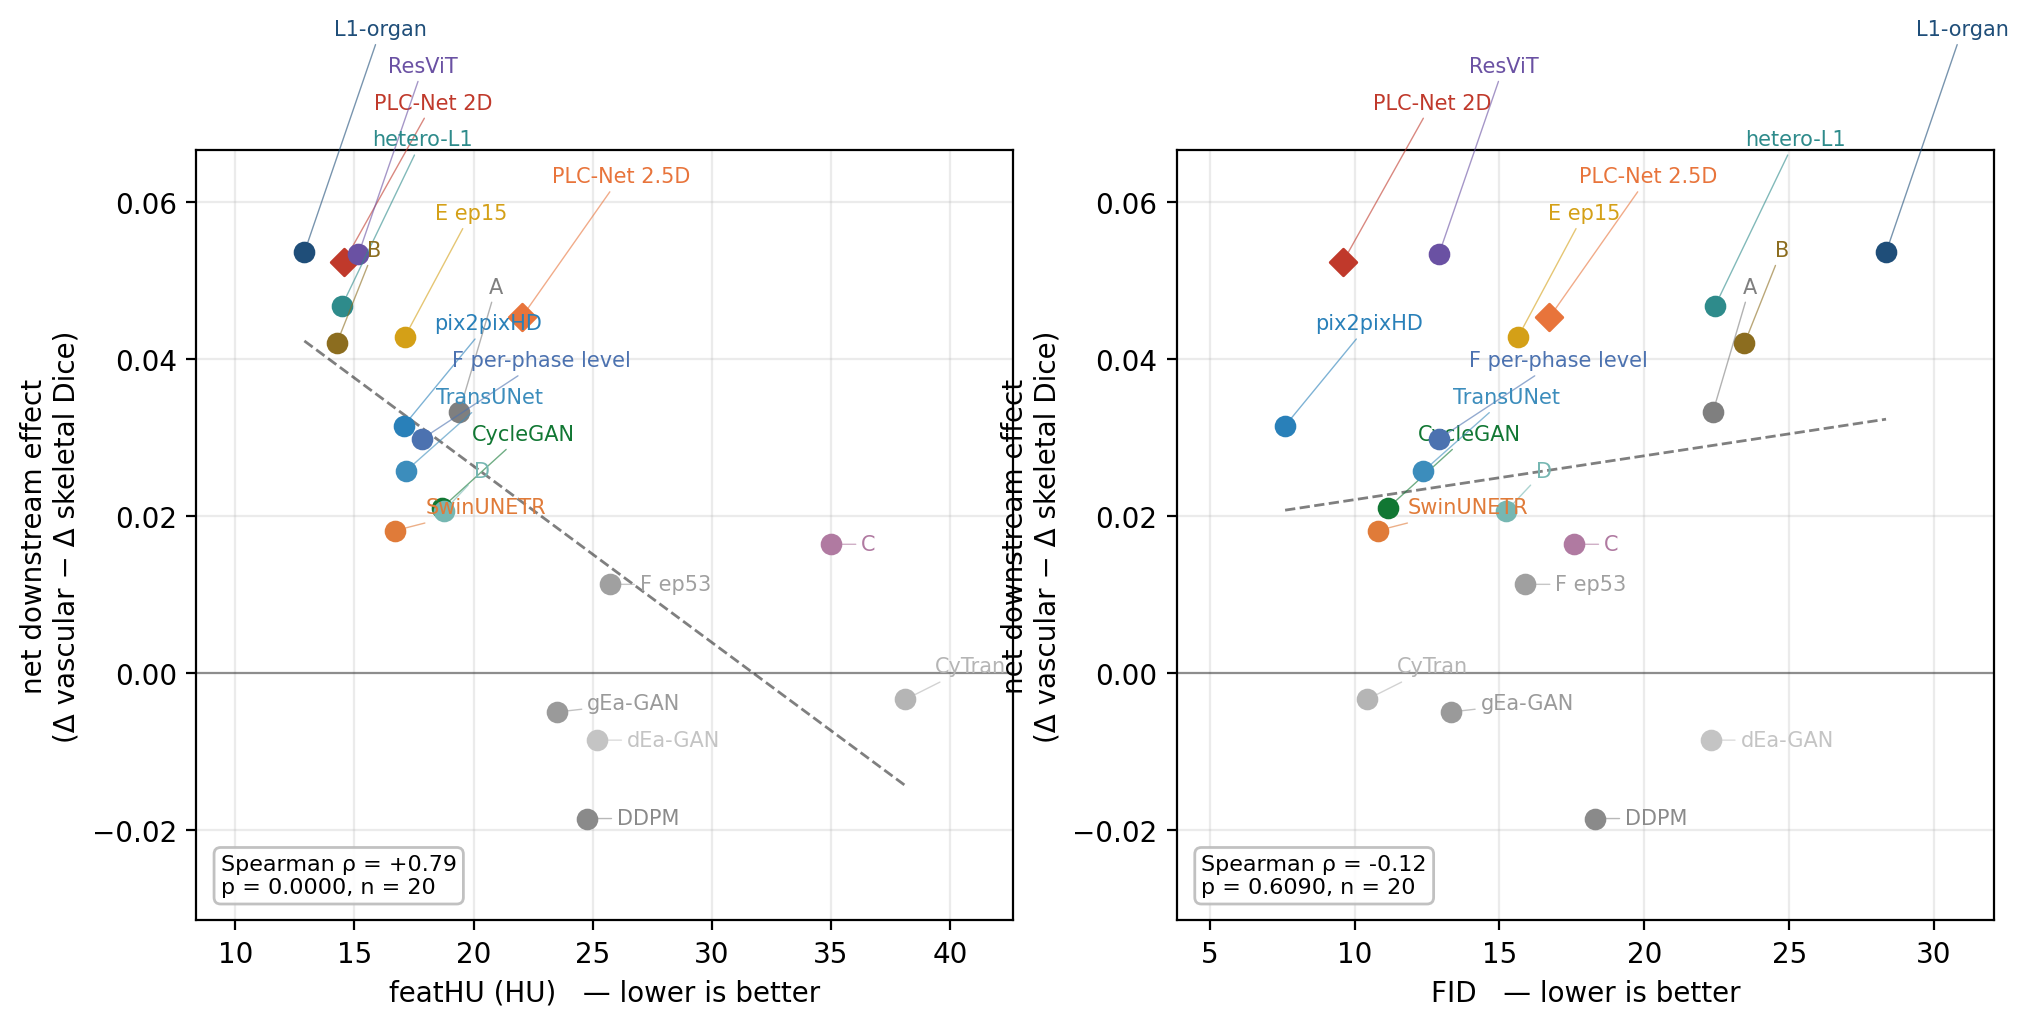
\includegraphics[width=0.95\textwidth]{synthesis/fig3_fidelity_vs_utility.png}
\caption{\lr{featHU} (چپ) و \lr{FID} (راست) در برابر اثر خالص پایین‌دستی برای \عدد{۲۰} بازوی وریدی. محورهای افقی مقادیر خام‌اند (کمتر بهتر)، اما $\rho$ روی معیار جهت‌دهی‌شده (بیشتر بهتر) محاسبه شده است؛ از این رو $\rho$ مثبت در نمودار چپ به‌صورت روند نزولی دیده می‌شود.}
\label{fig:syn-validity}
\end{figure}

این یافته با تمایزی که در بخش~\ref{sec:m-eval} مطرح شد سازگار است: معیارهای واقع‌نمایی توزیعی می‌سنجند که آیا تصویر تولیدشده شبیه تصاویر واقعی است، در حالی که \lr{featHU} می‌سنجد که آیا عدد هانسفیلد بافت درست است. برای وظیفه‌ای که به مرز میان بافت‌ها تکیه دارد، معیار دوم مرتبط‌تر است.

\subsection*{کنترل کیفیت داده}

ادعاهای سطح اندام در این بخش بر این فرض تکیه دارند که خطای هانسفیلد اندازه‌گیری‌شده خطای مدل است و نه باقی‌مانده‌ی ناهم‌ترازی جفت‌های تصویر. هم‌بستگی \lr{featHU} هر مورد با شاخص‌های کیفیت هم‌ترازسازی در \عدد{۲۰} مورد آزمون چنین است: هم‌بستگی متقابل استخوان $r = -0.09$، خطای مطلق استخوان $r = +0.25$ و دایس گاز روده $r = +0.11$؛ هیچ‌یک معنادار نیست. با \عدد{۲۰} مورد تنها هم‌بستگی‌هایی بزرگ‌تر از حدود \عدد{۰٫۴۴} در سطح \عدد{۰٫۰۵} قابل تشخیص‌اند؛ بنابراین این آزمون وابستگی قوی خطای هانسفیلد به ناهم‌ترازی را رد می‌کند، اما اثرهای کوچک‌تر را نه.

\subsection*{کیسه‌ی صفرا}

کیسه‌ی صفرا تنها اندامی است که همه‌ی بازوهای هم‌نهاده در آن دایس به‌روشنی کمتری از بازوی \lr{NCCT} دارند (برای \lr{PLC-Net} دوبعدی حدود \عدد{−۰٫۲۵}). این اندام در \عدد{۱۹} مورد ارزیابی می‌شود، زیرا در یک مورد آزمون در مرجع وجود ندارد. این یک شکست \emph{تشخیص} نیست: اندام در \عدد{۱۷} تا \عدد{۱۹} مورد از \عدد{۱۹} مورد یافت می‌شود. شکست، کم‌برآوردی نظام‌مند حجم است؛ میانه‌ی خطای علامت‌دار حجم برای \lr{NCCT} \عدد{−۵}٪، \lr{pix2pixHD} \عدد{−۸}٪، \lr{CycleGAN} \عدد{−۱۳}٪، \lr{L1}-اندام \عدد{−۱۸}٪، \lr{CyTran} \عدد{−۱۹}٪، \lr{PLC-Net} دوبعدی \عدد{−۳۲}٪، \lr{PLC-Net} \عدد{۲٫۵}~بعدی \عدد{−۳۷}٪، \lr{DDPM} \عدد{−۵۰}٪ و \lr{ResViT} \عدد{−۵۷}٪ است (شکل~\ref{fig:syn-gb}).

سازوکار این شکست اثبات نشده است. جمله‌ی تخاصمی به‌تنهایی آن را توضیح نمی‌دهد، زیرا \lr{pix2pixHD} و \lr{CycleGAN} نیز جمله‌ی تخاصمی دارند و کمترین خطای حجم را نشان می‌دهند. برای \lr{PLC-Net} یک فرضیه آن است که کیسه‌ی صفرا یکی از هشت اندام بردار سطح است و مدل ممکن است حفره‌ی آن را روشن کند، در حالی که در تصویر وریدی واقعی صفرای کم‌جذب باقی می‌ماند و مرز از دست می‌رود؛ این فرضیه اما خطای بزرگ \lr{ResViT} و \lr{DDPM} را توضیح نمی‌دهد. آزمون مستقیم آن، مقایسه‌ی \lr{HU} درون کیسه‌ی صفرا در تصویر هم‌نهاده و واقعی، انجام نشده است. همین اندام است که ترکیب وابسته به ماده‌ی حاجب را برای \lr{PLC-Net} دوبعدی، با وجود اثر \عدد{+۰٫۱۶۶} روی ورید باب، به حدود صفر می‌رساند.

\begin{figure}[H]
\centering
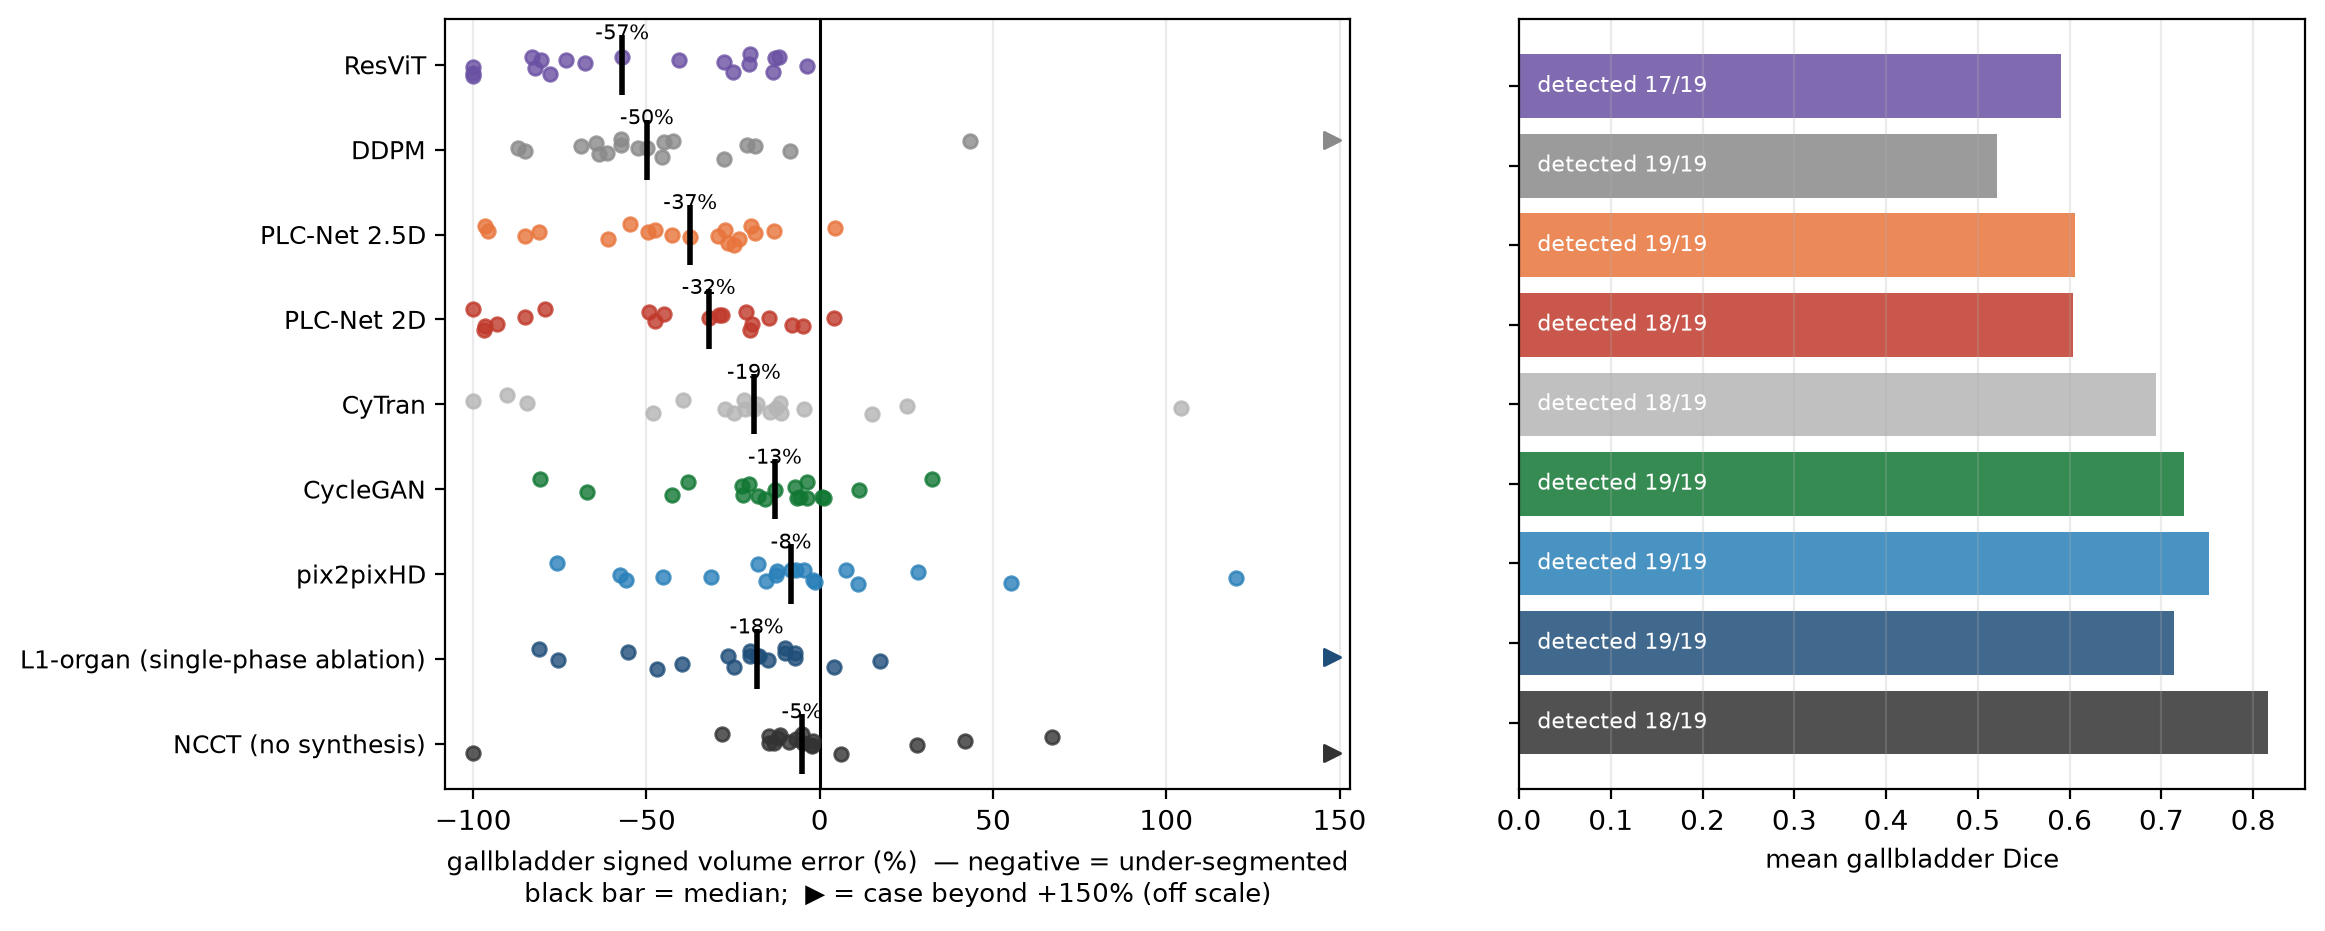
\includegraphics[width=0.95\textwidth]{synthesis/fig5_gallbladder.png}
\caption{کیسه‌ی صفرا. چپ: خطای علامت‌دار حجم برای هر مورد (میله‌ی سیاه: میانه؛ مقدار منفی یعنی حجم کمتر از مرجع؛ پیکان: موردی خارج از مقیاس بالای \عدد{+۱۵۰}٪). راست: دایس میانگین و تعداد مواردی که اندام یافت شده است.}
\label{fig:syn-gb}
\end{figure}

شکل~\ref{fig:syn-gb-img} مورد آزمونی را نشان می‌دهد که بیشترین افت دایس کیسه‌ی صفرا در آن رخ داده است؛ یعنی انتهای بد این توزیع، و نه یک مورد نمونه. روی تصویر بدون‌تزریق، بخش‌بند کیسه‌ی صفرا را کامل می‌یابد (دایس \عدد{۰٫۹۵}). در خروجی \lr{PLC-Net} دوبعدی و \عدد{۲٫۵}~بعدی و \lr{ResViT}، ناحیه‌ی کیسه‌ی صفرا همچنان تیره‌تر از کبد است، اما تباین آن با کبد کمتر از تصویر واقعی است و بخش‌بند تنها بخش کوچکی از آن را می‌یابد یا آن را نمی‌یابد (دایس \عدد{۰٫۰۶}، \عدد{۰٫۰۶} و \عدد{۰٫۰۰})؛ \lr{pix2pixHD}، \lr{CycleGAN} و \lr{L1}-اندام آن را حفظ می‌کنند (\عدد{۰٫۶۹}، \عدد{۰٫۷۲} و \عدد{۰٫۶۱}). این مشاهده با فرضیه‌ی روشن‌شدن حفره‌ی کیسه‌ی صفرا سازگار است، اما آن را اثبات نمی‌کند.

\begin{figure}[H]
\centering
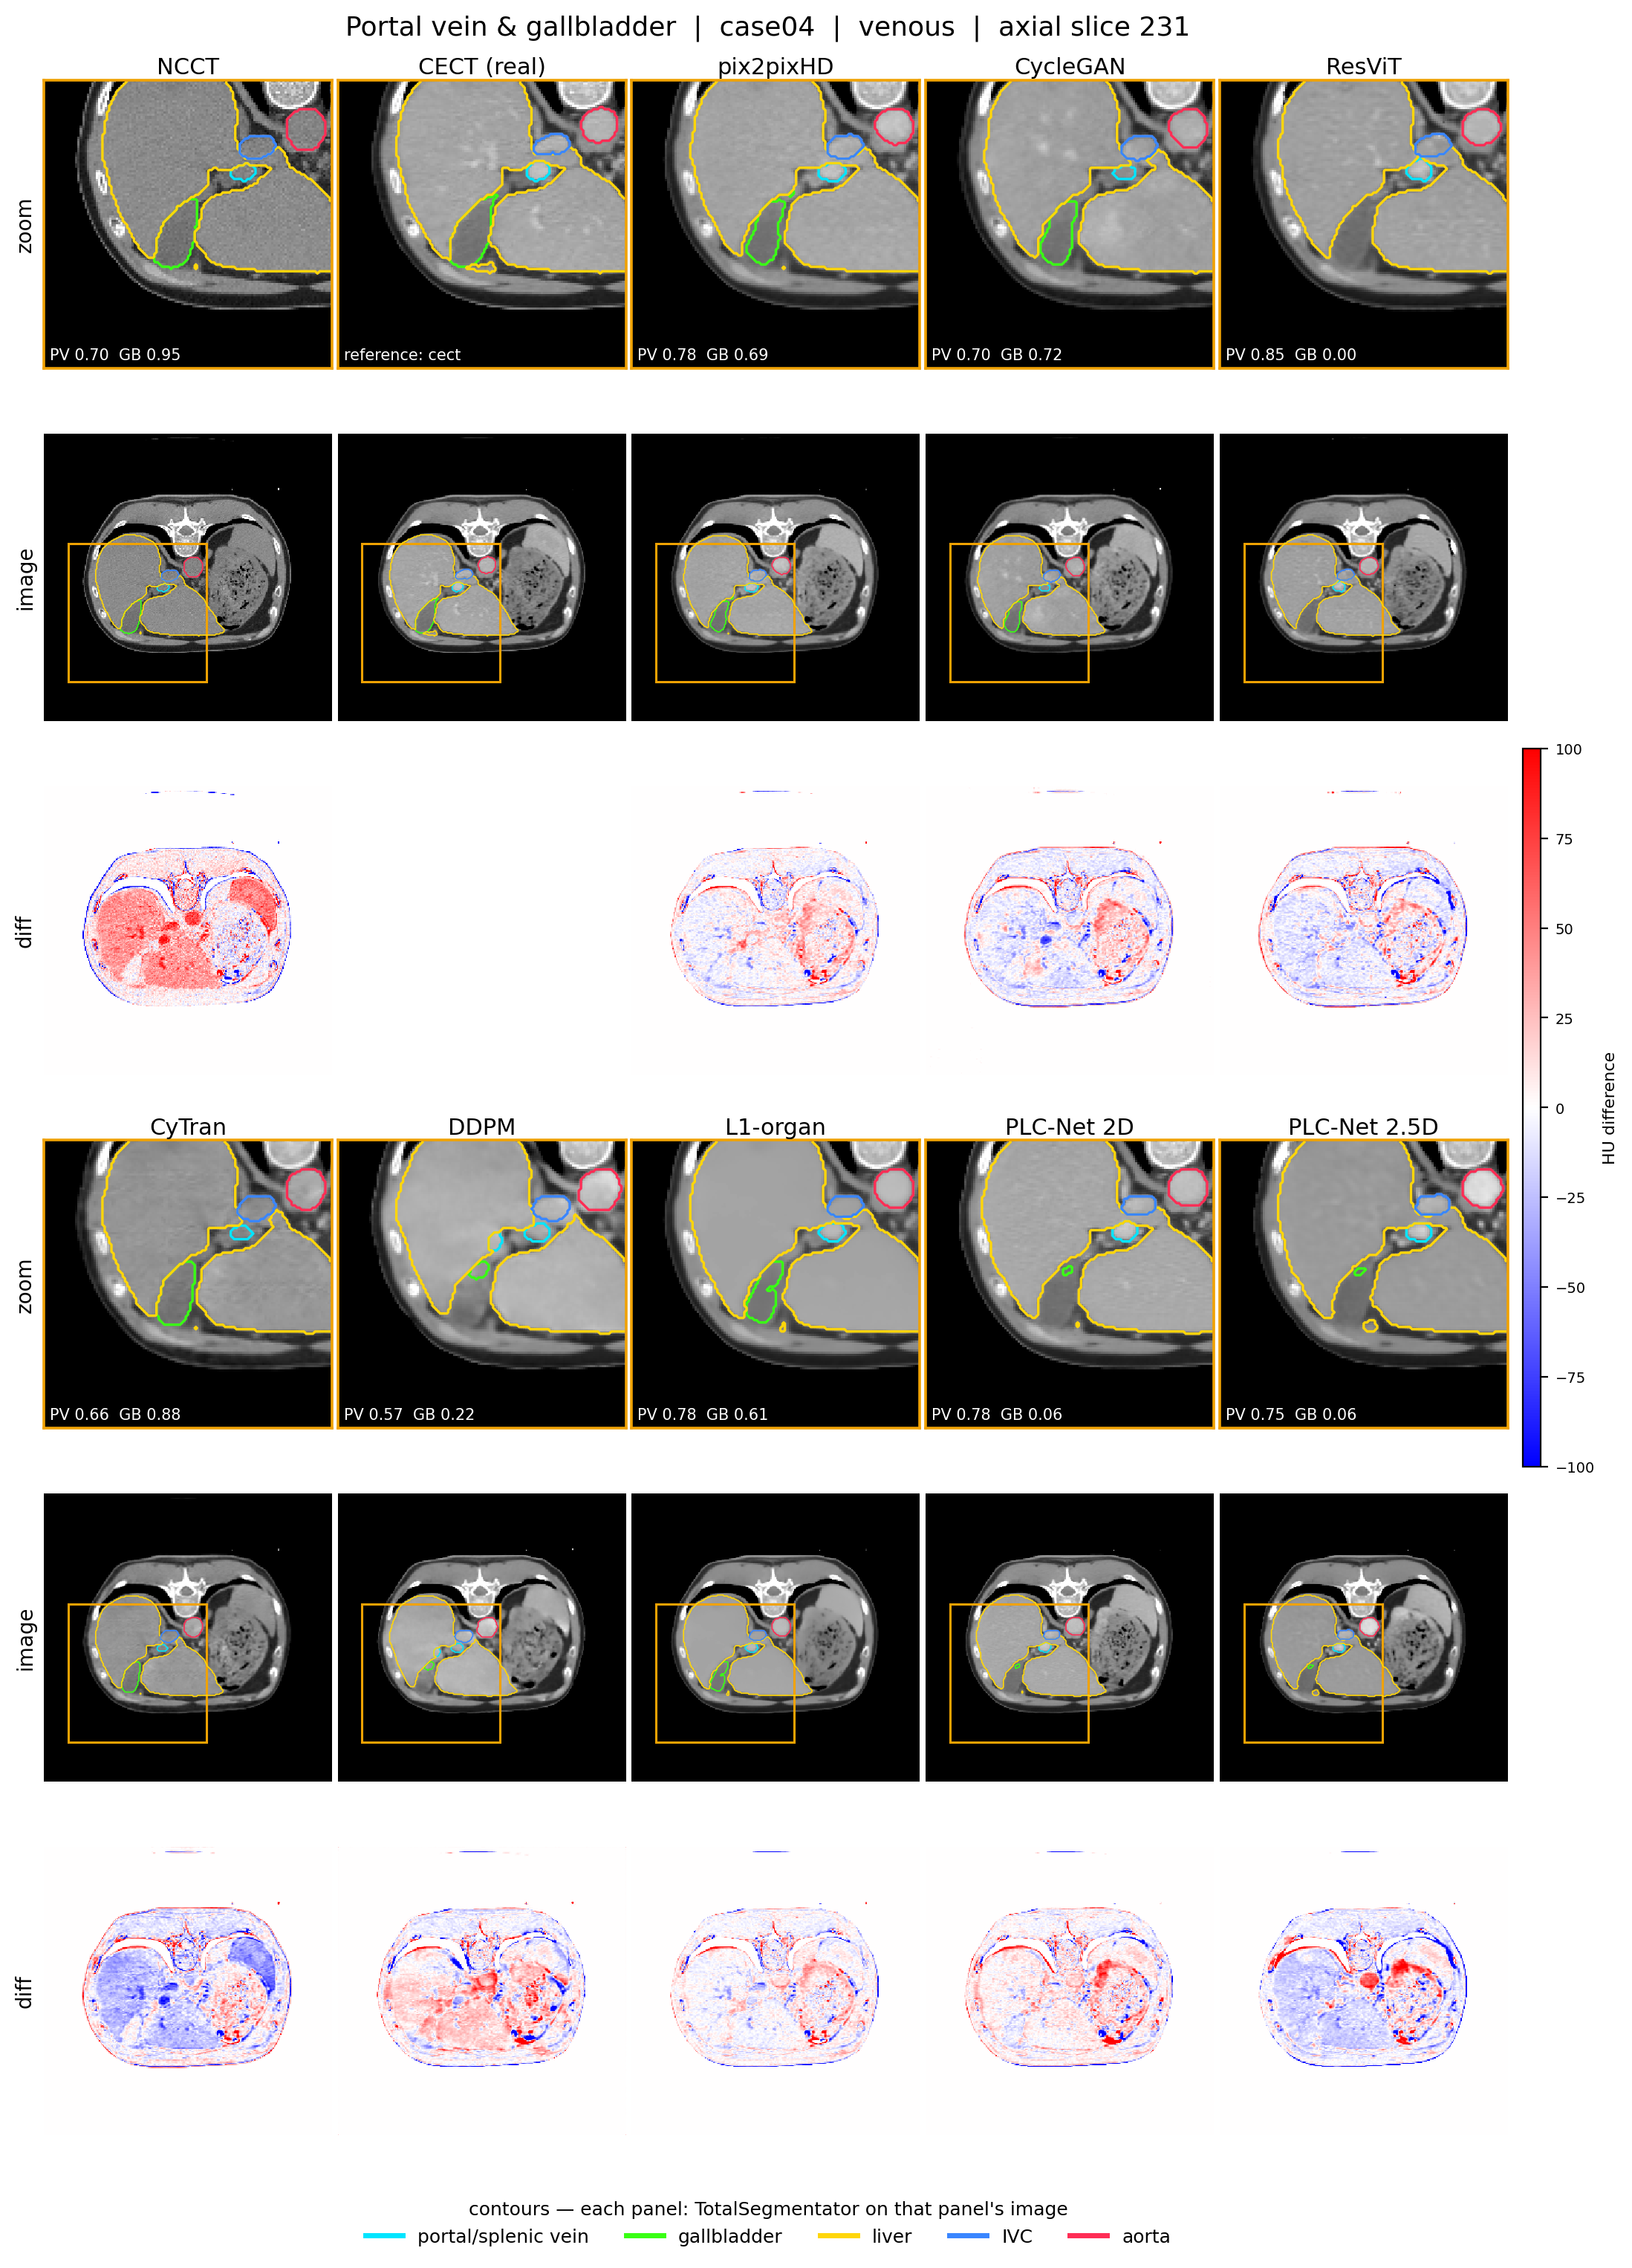
\includegraphics[width=\textwidth,height=0.72\textheight,keepaspectratio]{synthesis/qual_gallbladder_case04.png}
\caption{شکست کیسه‌ی صفرا در مورد آزمونی با بیشترین افت دایس کیسه‌ی صفرا، در تراز ورید باب و کیسه‌ی صفرا (خط سبز). پنجره، خطوط بخش‌بندی، اعداد دایس و ردیف تفاوت مانند شکل~\ref{fig:syn-cmp}.}
\label{fig:syn-gb-img}
\end{figure}


\section{ارزیابی مؤلفه‌ی تشخیص پویش}
\label{sec:e-phase}


مؤلفه‌ی تشخیص پویش در این پایان‌نامه یک مشارکت مستقل نیست؛ یک \emph{ابزار} است
که دو نقش مشخص دارد: دروازه‌بانی داده در بخش~\ref{sec:m-data}، و (مهم‌تر) تأمین
ابزار اندازه‌گیری برای معیارهای اصلی ارزیابی هم‌نهادی در بخش~\ref{sec:e-syn}؛
خلاصه‌ی نتیجه و دلیل انتخاب همان‌جا (بخش~\ref{sec:m-eval}) آمد. این بخش همان
مقایسه را با جزئیات کامل—فاصله‌ی اطمینان، آزمون‌های زوجی و تفکیک به‌ازای
پویش—می‌آورد. دو موضوع بررسی می‌شود. نخست، این خط‌کش روی بیمارانی که هرگز ندیده و در مقایسه با روش‌های منتشرشده در شرایط یکسان تا چه اندازه قابل‌اعتماد است؛ همین موضوع مبنای انتخاب مدل در بخش~\ref{sec:m-phase} هم بوده است. دوم، آزمایش مدل‌های بنیادین بخش~\ref{sec:m-phase} نشان می‌دهد بازنمایی‌های عمومی تصویر، بدون بخش‌بندی اندام، اطلاعات پویش را به همان اندازه در خود دارند یا نه.

\subsection*{پیکربندی ارزیابی}

همه‌ی روش‌های این بخش روی مجموعه‌ی آزمون بخش~\ref{sec:m-phase} سنجیده می‌شوند:
\عدد{۶۳} حجم از \عدد{۲۱} نوبت، از هر پویش \عدد{۲۱} حجم، که هیچ‌یک از مدل‌ها
بیماران آن را در آموزش ندیده‌اند. معیارها دقت، میانگین کلان \lr{F1} و \lr{F1}
به‌تفکیک پویش‌اند. فاصله‌ی اطمینان \عدد{۹۵} درصد
با بازنمونه‌گیری بوت‌استرپ\footnote{\lr{Bootstrap}}~\cite{efron1979bootstrap} و
\عدد{۲۰۰۰} تکرار برآورد می‌شود، و واحد بازنمونه‌گیری \emph{نوبت} است و نه حجم:
سه پویش یک بیمار از هم مستقل نیستند و بازنمونه‌گیری حجم‌ها، پهنای فاصله را کمتر
از واقع نشان می‌دهد. مقایسه‌ی دو روش زوجی و روی همان \عدد{۶۳} حجم انجام می‌شود
و معناداری آن با آزمون دقیق مک‌نمار\footnote{\lr{McNemar's test}}~\cite{mcnemar1947note}
سنجیده می‌شود، که تنها حجم‌هایی را به حساب می‌آورد که دو روش درباره‌شان
اختلاف دارند.

\subsection*{مقایسه با روش‌های منتشرشده}

از چهار روش دارای کد منبع منتشرشده، سه روش در این
مقایسه حضور دارند. دسته‌بند اندامی همان \lr{Segment-and-Classify}~\cite{phasedet2024xgboost} است که در بخش~\ref{sec:m-phase} برگزیده شد و روی مجموعه‌ی آموزش و اعتبارسنجی بازآموزی شده است، که برآوردی بدون نشت از
عملکرد ابزار اندازه‌گیری بخش~\ref{sec:e-syn} روی بیمار ناشناخته به دست می‌دهد. شبکه‌ی برش‌محور دائو و همکاران~\cite{zhou2021phaserecog} با پیکربندی
\lr{EfficientNet-B0} مخزن کد نویسندگان (پنجره‌ی \عدد{۴۰۰} هانسفیلدی با مرکز
\عدد{۵۰}، \عدد{۱۵} دوره‌ی آموزش، و رأی‌گیری اکثریت روی \عدد{۳۰} درصد برش‌های
تصادفی هر حجم) روی مجموعه‌ی آموزش بازآموزی شد و بهترین نقطه‌ی ذخیره با مجموعه‌ی
اعتبارسنجی انتخاب شد. تقسیم داده برای این شبکه نیز در سطح نوبت انجام شد و نه
در سطح برش، تا برش‌های یک حجم هم‌زمان در آموزش و آزمون حضور نداشته باشند.

مدل منتشرشده‌ی ریس و همکاران~\cite{tang2024interpretable} بدون بازآموزی اجرا شد.
این مدل برای سری \lr{DICOM} و نقاب‌های نسخه‌ی نخست \lr{TotalSegmentator} طراحی
شده است؛ در این‌جا نقاب‌های نسخه‌ی دوم به شناسه‌های نسخه‌ی نخست نگاشته شدند و
به‌جای دهلیز چپ، که در نسخه‌ی دوم برچسب مستقلی ندارد، کل قلب به کار رفت؛ همان
جایگزینی که در کد خود نویسندگان پیش‌بینی شده است. حساسیت نتیجه به ترتیب محورهای
حجم نیز بررسی شد و پیش‌بینی‌ها در \عدد{۶۲} حجم از \عدد{۶۳} حجم یکسان ماند. روش
یی و همکاران~\cite{tang2022deeplearning} از مقایسه کنار گذاشته شد، چون تنها وجود
تباین را تشخیص می‌دهد و میان پویش شریانی و وریدی تمایز نمی‌گذارد.
جدول~\ref{tab:phase-baselines} نتیجه‌ی این مقایسه را گزارش می‌کند.

\begin{table}[H]
\centering
\footnotesize
\caption{مقایسه‌ی دسته‌بند اندامی با روش‌های منتشرشده روی \عدد{۶۳} حجم آزمون. فاصله‌ی اطمینان \عدد{۹۵} درصد با قلم کوچک‌تر زیر هر مقدار آمده است. کد پویش: \عدد{۰} بدون‌تزریق، \عدد{۱} شریانی و \عدد{۲} وریدی. خروجی چهارکلاسه‌ی مدل‌هایی که روی داده‌ی دیگر آموزش دیده‌اند، به سه پویش موجود در مجموعه‌ی آزمون محدود شده است. بهترین مقدار پررنگ و دومین مقدار بهتر زیرخط‌دار است.}
\label{tab:phase-baselines}
\begin{tabular}{|p{3.9cm}|p{1.2cm}|p{2.1cm}|p{2.1cm}|p{1.1cm}|p{1.1cm}|p{1.1cm}|}
\hline
\textbf{روش} & \textbf{بازآموزی روی این داده} & \textbf{دقت} & \textbf{میانگین کلان \lr{F1}} & \textbf{\lr{F1} پویش \عدد{۰}} & \textbf{\lr{F1} پویش \عدد{۱}} & \textbf{\lr{F1} پویش \عدد{۲}} \\
\hline
دسته‌بند اندامی (\lr{Segment-and-Classify}، بازآموزی‌شده) & بله & \textbf{\عدد{۰٫۹۸۴}}\newline{\scriptsize\mbox{\عدد{۰٫۹۵۲--۱٫۰۰۰}}} & \textbf{\عدد{۰٫۹۸۴}}\newline{\scriptsize\mbox{\عدد{۰٫۹۵۲--۱٫۰۰۰}}} & \textbf{\عدد{۱٫۰۰}} & \textbf{\عدد{۰٫۹۸}} & \textbf{\عدد{۰٫۹۸}} \\
\hline
شبکه‌ی برش‌محور با نمونه‌برداری تصادفی~\cite{zhou2021phaserecog} & بله & \underline{\عدد{۰٫۹۶۸}}\newline{\scriptsize\mbox{\عدد{۰٫۹۲۱--۱٫۰۰۰}}} & \underline{\عدد{۰٫۹۶۸}}\newline{\scriptsize\mbox{\عدد{۰٫۹۱۸--۱٫۰۰۰}}} & \underline{\عدد{۰٫۹۸}} & \underline{\عدد{۰٫۹۵}} & \textbf{\عدد{۰٫۹۸}} \\
\hline
مدل تفسیرپذیر ریس و همکاران~\cite{tang2024interpretable} & خیر & \عدد{۰٫۸۲۵}\newline{\scriptsize\mbox{\عدد{۰٫۷۶۲--۰٫۸۸۹}}} & \عدد{۰٫۸۱۰}\newline{\scriptsize\mbox{\عدد{۰٫۷۱۸--۰٫۸۸۶}}} & \underline{\عدد{۰٫۹۸}} & \عدد{۰٫۶۵} & \underline{\عدد{۰٫۸۱}} \\
\hline
\end{tabular}
\end{table}

دسته‌بند اندامی تنها یک حجم از \عدد{۶۳} حجم را اشتباه تشخیص داد: یک حجم شریانی
که وریدی دسته‌بندی شد. هر سه روش دیگر نیز همین حجم را وریدی تشخیص دادند، و این
احتمالاً نشان می‌دهد با موردی مرزی از نظر زمان‌بندی تزریق سروکار داریم. دقت
اعتبارسنجی متقاطع همین مدل روی مجموعه‌ی آموزش و اعتبارسنجی \عدد{۰٫۹۶۰} بود که با
رقم آزمون سازگار است.

شبکه‌ی برش‌محور دائو و همکاران با دو خطا در رتبه‌ی بعدی قرار گرفت. تفاوت آن با
دسته‌بند اندامی تنها در یک حجم است و آزمون مک‌نمار تفاوتی نشان نمی‌دهد (مقدار
$p$ برابر \عدد{۱٫۰})؛ با این اندازه‌ی مجموعه‌ی آزمون، این دو روش را نمی‌توان
رتبه‌بندی کرد و هر دو نزدیک سقف‌اند. هر چهار سطر جدول همه‌ی \عدد{۲۱} حجم
بدون‌تزریق را درست تشخیص دادند؛ دشواری مسئله تقریباً به‌تمامی در تفکیک شریانی
از وریدی است.

مدل ریس و همکاران در این شرایط به دقت \عدد{۰٫۸۲۵} رسید، و اگر پیش‌بینی‌های پویش
تأخیری آن خطا شمرده شوند، دقت به \عدد{۰٫۷۳۰} کاهش می‌یابد (\عدد{۷} حجم). خطاهای
این مدل تقریباً یک‌سویه‌اند: \عدد{۱۰} خطا از \عدد{۱۱} خطا، حجمی شریانی را وریدی
تشخیص داده‌اند، و روی حجم‌های شریانی میانگین احتمال دو پویش شریانی و وریدی
تقریباً برابر است (\عدد{۰٫۴۰} و \عدد{۰٫۴۲}). یعنی مدل در این داده سطح تقویت
شریانی را به‌طور نظام‌مند کمتر از واقع می‌خواند. این رقم را نباید برآورد
منصفانه‌ای از توان خود روش دانست: مدل روی دستورالعمل تصویربرداری مرکزی دیگر و روی
نقاب‌های نسخه‌ی نخست \lr{TotalSegmentator} آموزش دیده است و در این‌جا با
نقاب‌های نگاشته‌شده، جایگزینی دهلیز چپ با کل قلب و حجم‌های برش‌خورده‌ی
هم‌ترازشده سنجیده شده است. سهم هر یک از این عوامل در این طرح قابل تفکیک نیست.

ارقام این جدول با ارقامی که مقاله‌ی هر روش گزارش کرده یکسان نیست. برای نمونه \lr{Segment-and-Classify} روی این داده، بدون بازآموزی، در پویش‌های شریانی و وریدی \lr{F1} بالاتری از رقم گزارش‌شده‌ی خود روی \lr{VinDr-Multiphase} دارد، در حالی که مدل ریس و همکاران به دقت \عدد{۰٫۷۳۰} می‌رسد، در برابر \عدد{۰٫۹۰۱} در مقاله. دلیل را نمی‌توان تفکیک کرد: مجموعه‌ی آزمون تنها \عدد{۲۱} نوبت دارد، پویش تأخیری در آن نیست، حجم‌ها برش‌خورده و هم‌ترازشده‌اند، و برای مدل ریس و همکاران نقاب‌ها از نسخه‌ی دیگری از \lr{TotalSegmentator} نگاشته شده‌اند. نتیجه‌ی عملی همان نیازمندی دوم بخش~\ref{sec:m-phase} است: رقم گزارش‌شده‌ی یک مدل برآورد قابل‌اتکایی از عملکرد آن روی داده‌ی تازه نیست و انتخاب باید روی خود داده انجام شود.

\subsection*{آزمایش مدل‌های بنیادین: اطلاعات پویش در بازنمایی‌های عمومی تصویر}


جدول~\ref{tab:phase-featmaps} نتیجه‌ی شش ترکیب رمزگذار و سر دسته‌بند را گزارش
می‌کند.

\begin{table}[H]
\centering
\footnotesize
\caption{کاوش خطی بازنمایی‌های عمومی تصویر برای تشخیص پویش. دقت اعتبارسنجی متقاطع روی مجموعه‌ی آموزش و اعتبارسنجی به‌صورت میانگین و انحراف معیار پنج تا آمده است، و ارقام آزمون روی همان \عدد{۶۳} حجم جدول~\ref{tab:phase-baselines} و با همان کد پویش محاسبه شده‌اند. برای سر لایه‌ی خطی، پیش‌بینی‌های حجم‌به‌حجم ذخیره نشده و فاصله‌ی اطمینان در دسترس نیست. بهترین مقدار پررنگ و دومین مقدار بهتر زیرخط‌دار است.}
\label{tab:phase-featmaps}
\begin{tabular}{|p{1.35cm}|p{1.5cm}|p{2.25cm}|p{1.9cm}|p{1.9cm}|p{0.9cm}|p{0.9cm}|p{0.9cm}|}
\hline
\textbf{رمزگذار} & \textbf{سر دسته‌بند} & \textbf{دقت اعتبارسنجی متقاطع} & \textbf{دقت آزمون} & \textbf{میانگین کلان \lr{F1} آزمون} & \textbf{\lr{F1} پویش \عدد{۰}} & \textbf{\lr{F1} پویش \عدد{۱}} & \textbf{\lr{F1} پویش \عدد{۲}} \\
\hline
\lr{DINOv2} & \lr{LDA} & \mbox{\textbf{\عدد{۰٫۸۱۵±۰٫۰۴۷}}} & \textbf{\عدد{۰٫۸۴۱}}\newline{\scriptsize\mbox{\عدد{۰٫۷۷۸--۰٫۹۲۱}}} & \textbf{\عدد{۰٫۸۴۱}}\newline{\scriptsize\mbox{\عدد{۰٫۷۶۹--۰٫۹۲۰}}} & \textbf{\عدد{۱٫۰۰}} & \textbf{\عدد{۰٫۷۵}} & \textbf{\عدد{۰٫۷۷}} \\
\hline
\lr{DINOv2} & \lr{PCA} و \lr{LDA} & \mbox{\underline{\عدد{۰٫۷۶۱±۰٫۰۴۰}}} & \عدد{۰٫۷۴۶}\newline{\scriptsize\mbox{\عدد{۰٫۶۶۷--۰٫۸۲۵}}} & \عدد{۰٫۷۴۷}\newline{\scriptsize\mbox{\عدد{۰٫۶۵۷--۰٫۸۲۷}}} & \underline{\عدد{۰٫۹۸}} & \عدد{۰٫۶۷} & \عدد{۰٫۶۰} \\
\hline
\lr{DINOv2} & لایه‌ی خطی & \mbox{\عدد{۰٫۷۵۵±۰٫۰۳۵}} & \underline{\عدد{۰٫۷۶۲}} & \underline{\عدد{۰٫۷۶۱}} & \textbf{\عدد{۱٫۰۰}} & \عدد{۰٫۶۷} & \underline{\عدد{۰٫۶۲}} \\
\hline
\lr{MedViT} & \lr{LDA} & \mbox{\عدد{۰٫۷۱۵±۰٫۰۵۲}} & \عدد{۰٫۷۴۶}\newline{\scriptsize\mbox{\عدد{۰٫۶۸۳--۰٫۸۱۰}}} & \عدد{۰٫۷۲۸}\newline{\scriptsize\mbox{\عدد{۰٫۶۴۰--۰٫۸۰۲}}} & \underline{\عدد{۰٫۹۸}} & \underline{\عدد{۰٫۷۱}} & \عدد{۰٫۵۰} \\
\hline
\lr{MedViT} & \lr{PCA} و \lr{LDA} & \mbox{\عدد{۰٫۶۷۴±۰٫۰۳۱}} & \عدد{۰٫۶۸۳}\newline{\scriptsize\mbox{\عدد{۰٫۶۱۹--۰٫۷۴۶}}} & \عدد{۰٫۶۷۲}\newline{\scriptsize\mbox{\عدد{۰٫۵۹۷--۰٫۷۴۴}}} & \underline{\عدد{۰٫۹۸}} & \عدد{۰٫۶۳} & \عدد{۰٫۴۱} \\
\hline
\lr{MedViT} & لایه‌ی خطی & \mbox{\عدد{۰٫۶۶۶±۰٫۰۳۰}} & \عدد{۰٫۵۸۷} & \عدد{۰٫۵۴۳} & \عدد{۰٫۸۴} & \عدد{۰٫۵۲} & \عدد{۰٫۲۷} \\
\hline
\end{tabular}
\end{table}

بهترین ترکیب، \lr{DINOv2} با تحلیل تشخیصی خطی، به دقت آزمون \عدد{۰٫۸۴۱} رسید، و
دقت اعتبارسنجی متقاطع آن (\عدد{۰٫۸۱۵}) نشان می‌دهد این رقم حاصل یک تقسیم
خوش‌اقبال نیست. در هر دو رمزگذار، کاهش ابعاد با تحلیل مؤلفه‌های اصلی دقت را پایین
آورد و لایه‌ی خطی نیز از تحلیل تشخیصی خطی بهتر عمل نکرد؛ یعنی بخشی از اطلاعات
پویش در مؤلفه‌هایی نشسته است که بیشترین وردایی را ندارند، و افزودن پراسنجه
آموزش‌پذیر به سر دسته‌بند آن را بازیابی نمی‌کند.

الگوی خطا در همه‌ی ترکیب‌ها مشابه است. در پنج ترکیب از شش ترکیب، \lr{F1} پویش
بدون‌تزریق دست‌کم \عدد{۰٫۹۸} است، در حالی که \lr{F1} پویش شریانی یا وریدی در
هیچ ترکیبی از \عدد{۰٫۷۷} فراتر نمی‌رود. ده خطای بهترین ترکیب در ده نوبت متفاوت
پخش شده‌اند (شش حجم شریانی که وریدی و چهار حجم وریدی که شریانی تشخیص داده شدند)
و هیچ‌یک از آن‌ها را دسته‌بند اندامی یا شبکه‌ی برش‌محور اشتباه نکرده است.
\lr{MedViT} با تحلیل تشخیصی خطی، علاوه بر دقت پایین‌تر، سوگیری آشکاری دارد:
\عدد{۱۲} خطا از \عدد{۱۶} خطای آن، حجم وریدی را شریانی تشخیص داده‌اند.

در مقایسه‌ی زوجی، دقت بهترین ترکیب \عدد{۱۴٫۳} واحد درصد کمتر از دسته‌بند اندامی
است (فاصله‌ی اطمینان \عدد{۴٫۸--۲۲٫۲})؛ از \عدد{۱۱} حجمی که دو روش درباره‌شان
اختلاف دارند، دسته‌بند اندامی \عدد{۱۰} حجم را درست تشخیص داده است (مقدار $p$
آزمون مک‌نمار برابر \عدد{۰٫۰۱۲}). فاصله با شبکه‌ی برش‌محور دائو و همکاران
\عدد{۱۲٫۷} واحد درصد است (\عدد{۳٫۲--۲۰٫۶}؛ مقدار $p$ برابر \عدد{۰٫۰۳۹}). با
تصحیح بونفرونی برای سه مقایسه با روش‌های منتشرشده، تنها تفاوت با دسته‌بند اندامی
معنادار می‌ماند. در مقابل، این ترکیب با مدل ریس و همکاران تفاوت معناداری ندارد
(\عدد{۱٫۶} واحد درصد به سود \lr{DINOv2}؛ مقدار $p$ برابر \عدد{۱٫۰})، و برتری
\lr{DINOv2} بر \lr{MedViT} با همان سر دسته‌بند (\عدد{۹٫۵} واحد درصد) نیز در این
اندازه‌ی نمونه معنادار نیست (مقدار $p$ برابر \عدد{۰٫۲۴}).

یک تبیین محتمل آن است که ورود ماده‌ی حاجب تغییری سراسری و پرتباین ایجاد می‌کند که حتی رمزگذاری آموزش‌دیده روی تصاویر طبیعی آن را بازتاب می‌دهد، در حالی که تفکیک شریانی از وریدی به مقایسه‌ی سطح \lr{HU} میان چند ساختار کوچک وابسته است. در این پیکربندی چند عامل (پنجره‌ی شدت پهن، بازنمونه‌برداری به \عدد{۱۲۸} حجم‌دانه و ادغام میانگین) این اطلاعات ظریف را رقیق می‌کنند؛ آزمایش سهم آن‌ها را جدا نمی‌کند و از آن نمی‌توان نتیجه گرفت که بازنمایی‌های عمومی \emph{در هر پیکربندی} ناکافی‌اند.


نتیجه‌ی عملی این آزمایش برای پایان‌نامه روشن است. یک بازنمایی عمومی، پویش
بدون‌تزریق را به‌خوبی تشخیص می‌دهد اما در تفکیک شریانی از وریدی، که ظریف‌ترین
بخش مسئله است، به‌طور معنادار از دسته‌بند اندامی عقب می‌ماند. چون خط‌کش ارزیابی
هم‌نهادی باید دقیقاً همین تمایز را بسنجد، این نتیجه تعیین می‌کند که خط‌کش باید از
میانه‌های \lr{HU} سطح‌اندام ساخته شود و نه از یک بازنمایی عمومی. حذف وابستگی به
بخش‌بندی در شرایط این مطالعه هزینه‌ی معناداری در دقت دارد، در حالی که نقاب‌های
اندام به‌هرحال برای هم‌ترازسازی و وزن‌دهی زیان هم‌نهادی تولید می‌شوند؛ از این رو
دسته‌بند اندامی حفظ شد.

\subsection*{نقش این مدل در ارزیابی هم‌نهادی}


ارزش اصلی این مؤلفه در جای دیگری است. همان بردار \عدد{۱۶} بعدی و همان
دسته‌بند، دو معیار اصلی جدول~\ref{tab:syn-metrics} را می‌سازند:

\begin{itemize}
\item \مهم{\lr{featHU}} از فاصله‌ی همین بردار میان تصویر هم‌نهاده و تصویر واقعی
به دست می‌آید و مستقیم‌ترین سنجه‌ی بازسازی سطح تقویت است.
\item \مهم{\lr{phase} و \lr{prob}} خروجی همین دسته‌بند روی تصویر هم‌نهاده‌اند و
می‌پرسند آیا تصویر تولیدشده اساساً به پویش درخواست‌شده \emph{تعلق دارد}.
\end{itemize}

به این ترتیب، مدلی که برای آماده‌سازی داده برگزیده شد، مسئله‌ی سنجش را نیز
حل می‌کند. اعتبار این کاربرد به دقت مطلق دسته‌بند وابسته نیست بلکه به
\emph{ثبات} آن وابسته است: چون یک خط‌کش واحد روی خروجی همه‌ی مدل‌های
مقایسه‌شده اعمال می‌شود، هر سوگیری سامانهاتیک آن میان مدل‌ها مشترک است و
رتبه‌بندی را جابه‌جا نمی‌کند.

یک قید باید کنار این استدلال گذاشته شود. نسخه‌ای از دسته‌بند که در ارزیابی هم‌نهادی
به کار می‌رود، روی هر \عدد{۴۱۰} حجم آموزش دیده است؛ یعنی روی تصاویر واقعی همه‌ی
\عدد{۱۳۷} نوبت، از جمله بیماران تقسیم آزمون هم‌نهادی. دقت خارج‌ازتای\footnote{\lr{Out-of-fold}}
همین دستورالعمل روی این \عدد{۴۱۰} حجم \عدد{۰٫۹۷۱} است و با دقت \عدد{۰٫۹۸۴} نسخه‌ی
بازآموزی‌شده روی بیماران ناشناخته هم‌خوان است؛ پس خط‌کش به داده‌ی تازه تعمیم
می‌یابد. با این حال، معیارهای \lr{phase} و \lr{prob} روی تصویر هم‌نهاده بیمارانی
سنجیده می‌شوند که تصویر واقعی‌شان در آموزش دسته‌بند حضور داشته است، و مقدار مطلق
آن‌ها ممکن است اندکی خوش‌بینانه باشد. انتظار می‌رود این اثر عمدتاً میان همه‌ی
مدل‌های هم‌نهادی مشترک باشد، هرچند نمی‌توان کاملاً رد کرد که به سود مدل‌هایی تمام
شود که خروجی‌شان به تصویر واقعی همان بیمار نزدیک‌تر است. معیار \lr{featHU} از این
قید مصون است، چون تنها از استخراج ویژگی استفاده می‌کند و دسته‌بند در آن نقشی
ندارد. بازآموزی دسته‌بند بدون بیماران تقسیم آزمون هم‌نهادی و امتیازدهی دوباره، این
قید را برطرف می‌کند.

دو قید بر خواندن ارقام این بخش اثر می‌گذارند: ارزیابی درون‌سازمانی است و پویش تأخیری را پوشش نمی‌دهد، و مدل‌هایی که بدون بازآموزی اجرا شدند در شرایطی سنجیده شده‌اند که با ورودی اصلی آن‌ها یکسان نیست.


\section{ارزیابی مؤلفه‌ی هم‌ترازسازی}
\label{sec:e-reg}

این بخش مؤلفه‌ی هم‌ترازسازی (بخش~\ref{sec:m-reg}) را ارزیابی می‌کند. قراردادهای گزارش و معیارها در بخش~\ref{sec:e-setup-reg} تعریف شده‌اند و دو مطالعه‌ی حذفی این مؤلفه در بخش~\ref{sec:e-ablation} آمده‌اند؛ این بخش داده‌ی واجد شرط و اندازه‌ی مسئله، مقایسه با روش‌های موجود، اثر پیش‌پردازش بر آن‌ها، گذر اختیاری غیرصلب و هزینه‌ی محاسباتی را گزارش می‌کند.


\subsection*{داده‌ی واجد شرط}

از \عدد{۲۶۵} نوبت مجموعه‌داده، تنها \عدد{۱۶۹} نوبت (\عدد{۶۳٫۸} درصد) سری
بدون‌تزریق دارند. چون پویش بدون‌تزریق در سراسر این زنجیره‌ی مرجع ثابت است،
\عدد{۹۶} نوبت باقی‌مانده پیش از هر هم‌ترازسازی کنار گذاشته می‌شوند. همین عدد، و
نه کیفیت هم‌ترازی، سقف تعداد جفت‌های آموزشی هم‌نهادی را تعیین می‌کند.

تبدیل \lr{DICOM} به \lr{NIfTI} روی هر \عدد{۷۷۲} حجم بدون خطا انجام شد و بررسی
خودکار سلامت بخش‌بندی \عدد{۷۷۱} حجم را پذیرفت. تنها حجم ردشده هر سه شرط این
بررسی را هم‌زمان نقض می‌کرد: هیچ اندام مرجعی در آن شناسایی نشده بود، برچسب ستون
فقرات نداشت و نقاب آن خالی بود؛ یعنی دقیقاً همان خرابی که این بررسی برای
شناسایی‌اش طراحی شده است.

\subsection*{اندازه‌ی ناهم‌ترازی پیش از هم‌ترازسازی}

پیش از تفسیر نتایج، اندازه‌ی مسئله باید روشن شود. جابه‌جایی مرکز اندام‌ها میان
پویش بدون‌تزریق و پویش‌های دیگر، در حالت معمول \عدد{۲٫۷۹} میلی‌متر است؛ تنها در
\عدد{۱۰} درصد سری‌ها از \عدد{۱۰٫۵} میلی‌متر بیشتر می‌شود و بیشینه‌ی آن
\عدد{۲۹٫۸} میلی‌متر است. گام هم‌ترازی درشت مرکز جرم تنها وقتی جابه‌جایی اعمال
می‌کند که جابه‌جایی برآوردشده از یک آستانه‌ی کمینه بزرگ‌تر باشد؛ این شرط در راستای
سر به پا در \عدد{۱۲٫۴} درصد و در صفحه‌ی مقطع در \عدد{۸٫۸} درصد سری‌ها برقرار شد.

به بیان دیگر، پویش‌های این مجموعه‌داده در حدود \عدد{۸۷} درصد موارد از پیش تقریباً
هم‌موقعیت‌اند. مسئله‌ی اصلی در این داده جابه‌جایی‌های بزرگ و فراگیر نیست، بلکه
ناهم‌ترازی‌های چندمیلی‌متری و شکست‌های پراکنده است؛ این نکته در تفسیر جدول‌های
بعد، به‌ویژه اثر پیش‌پردازش بر روش‌های موجود، تعیین‌کننده است.

\subsection*{مقایسه با روش‌های موجود}

جدول~\ref{tab:reg-compare} مسیر پیشنهادی را کنار چهار روش هم‌ترازسازی شناخته‌شده
قرار می‌دهد: \lr{ANTs-SyN}~\cite{avants2008}، مدل آموخته‌شده‌ی
\lr{uniGradICON}~\cite{tian2023} با و بدون بهینه‌سازی تکمیلی، و
\lr{DEEDS}~\cite{heinrich2013}. «بهینه‌سازی تکمیلی» یعنی \عدد{۵۰} گام بهینه‌سازی
روی هر جفت، پس از پیش‌بینی مدل آموخته‌شده. روش‌های موجود یک‌بار روی خروجی
پیش‌پردازش این پایان‌نامه اجرا شده‌اند و دو روش از آن‌ها روی حجم خام نیز در جدول
آمده‌اند؛ مقایسه‌ی کامل خام و پیش‌پردازش‌شده در زیربخش «اثر پیش‌پردازش بر روش‌های
موجود» می‌آید.

\begin{table}[H]
\centering
\footnotesize
\caption{مقایسه با روش‌های موجود روی مجموعه‌ی مشترک (\عدد{۲۶} نوبت، \عدد{۵۷۴} مورد مقایسه) با خط‌کش ارزیابی یکسان. همه‌ی ستون‌ها مقدار معمول‌اند؛ برای دایس مقدار بیشتر و برای بقیه‌ی ستون‌ها مقدار کمتر بهتر است. تاخوردگی برای روش صلب بنا به تعریف صفر است. زمان به‌ازای هر جفت پویش است؛ زمان مسیر صلب از اجرای همان تابع هدف در جدول~\ref{tab:reg-objective} و زمان ردیف \lr{B}-اسپلاین مجموع زمان مسیر صلب و این گذر است. جزئیات رویه‌ی اندازه‌گیری زمان در پیوست~\ref{sec:app-cost} آمده است. خروجی مسیر صلب از اجرایی گرفته شده که گام هم‌ترازی درشت مرکز جرم هنوز در آن فعال بود؛ حذف این گام تفاوت معناداری در دقت ایجاد نمی‌کند (جدول~\ref{tab:reg-ablation}). بهترین مقدار پررنگ و دومین مقدار بهتر زیرخط‌دار است.}
\label{tab:reg-compare}
\begin{tabular}{|p{3.6cm}|C{1.9cm}|C{1.9cm}|C{1.9cm}|C{1.9cm}|C{1.9cm}|}
\hline
\textbf{روش} & \textbf{دایس} & \textbf{خطای مرکز (میلی‌متر)} & \textbf{فاصله‌ی مرزها (میلی‌متر)} & \textbf{تاخوردگی (درصد)} & \textbf{زمان (ثانیه)} \\
\hline
\multicolumn{6}{|l|}{\emph{مسیر پیشنهادی (بدون وزن آموخته‌شده)}} \\
\hline
مسیر صلب پیشنهادی & \عدد{۰٫۸۱۵} & \عدد{۲٫۰۹} & \عدد{۳٫۳۵} & \عدد{۰} & \underline{\عدد{۲۸}} \\
\hline
مسیر صلب \lr{+} پالایش \lr{B}-اسپلاین & \underline{\عدد{۰٫۸۵۹}} & \عدد{۱٫۳۰} & \عدد{۳٫۰۰} & \عدد{۰٫۰۰} & \عدد{۶۹۷} \\
\hline
\multicolumn{6}{|l|}{\emph{روش‌های موجود، روی خروجی پیش‌پردازش این پایان‌نامه}} \\
\hline
\lr{ANTs-SyN} & \عدد{۰٫۸۰۹} & \عدد{۱٫۵۵} & \عدد{۳٫۰۰} & \عدد{۰٫۰۰} & \عدد{۸۸} \\
\hline
\lr{uniGradICON} & \عدد{۰٫۷۹۴} & \عدد{۱٫۳۳} & \عدد{۳٫۰۰} & \عدد{۰٫۰۰} & \textbf{\عدد{۱۱}} \\
\hline
\lr{uniGradICON} با بهینه‌سازی تکمیلی & \عدد{۰٫۸۳۲} & \underline{\عدد{۱٫۱۲}} & \underline{\عدد{۲٫۶۰}} & \عدد{۰٫۰۰} & \عدد{۱۶۹} \\
\hline
\lr{DEEDS} & \textbf{\عدد{۰٫۸۸۶}} & \textbf{\عدد{۱٫۰۱}} & \textbf{\عدد{۲٫۱۲}} & \عدد{۲٫۶۵} & \عدد{۲۵۷} \\
\hline
\multicolumn{6}{|l|}{\emph{روش‌های موجود، روی حجم خام}} \\
\hline
\lr{DEEDS} & \عدد{۰٫۸۸۰} & \عدد{۱٫۱۷} & \عدد{۲٫۱۲} & \عدد{۱٫۹۴} & \عدد{۱۰۳} \\
\hline
\lr{uniGradICON} & \عدد{۰٫۷۳۶} & \عدد{۱٫۷۵} & \عدد{۳٫۳۵} & \عدد{۰٫۰۰} & \عدد{۱۰} \\
\hline
\end{tabular}
\end{table}

\مهم{در دقت، \lr{DEEDS} به‌وضوح جلوتر است.} مسیر صلب در \عدد{۶۳} مورد از
\lr{DEEDS} بهتر و در \عدد{۵۰۵} مورد بدتر است ($p$ کمتر از \عدد{۰٫۰۰۱})، و هیچ
خوانشی از این داده ادعای هم‌رده‌بودن دقت آن دو را پشتیبانی نمی‌کند. اما \lr{DEEDS}
در حالت معمول \عدد{۲٫۶۵} درصد حجم‌دانه‌های درون نقاب را تا می‌کند؛ تغییرشکل در آن
نواحی از نظر فیزیکی نامعتبر است و بافتی می‌سازد که در بدن بیمار وجود ندارد. برای
کاربرد این پایان‌نامه، یعنی ساخت جفت‌های آموزشی هم‌نهادی، نبودِ تاخوردگی یک الزام است.
با این حال بهترین دقت کل این مطالعه، دایس \عدد{۰٫۸۸۶}، روی خروجی پیش‌پردازش همین
پایان‌نامه به دست آمده است.

\مهم{در برابر مدل آموخته‌شده، نتیجه برابری است و نه برتری.} مقدار معمول دایس مسیر
صلب (\عدد{۰٫۸۱۵}) از \lr{uniGradICON} (\عدد{۰٫۷۹۴}) بالاتر است، اما مقایسه‌ی
مورد به مورد این تفاوت را تأیید نمی‌کند (\عدد{۲۹۸} بهتر در برابر \عدد{۲۷۹} بدتر؛
$p$ برابر \عدد{۰٫۴۵}). ادعای درست این است که یک مسیر صلبِ بدون آموزش با یک مدل
هم‌ترازسازی آموخته‌شده روی مجموعه‌داده‌های متعدد تفاوت معناداری ندارد؛ نه این‌که از
آن بهتر است. نسخه‌ی همان مدل با بهینه‌سازی تکمیلی از مسیر صلب به‌طور معنادار
دقیق‌تر است (\عدد{۲۰۳} بهتر در برابر \عدد{۳۷۲} بدتر برای مسیر صلب؛ $p$ کمتر از
\عدد{۰٫۰۰۱}).

\مهم{با گذر اختیاری \lr{B}-اسپلاین، مسیر پیشنهادی به گروه روش‌های غیرصلب بدون
تاخوردگی می‌رسد.} این ردیف بالاترین مقدار معمول دایس را در میان روش‌های بدون
تاخوردگی دارد، اما مقدار معمول به‌تنهایی مبنای رتبه‌بندی نیست؛ مقایسه‌ی مورد به
مورد، الگوی اثر به تفکیک اندام و هزینه‌ی این گذر در زیربخش «گذر اختیاری پالایش
غیرصلب» گزارش می‌شود.

\subsection*{تفکیک به‌ازای گروه اندام و اندام}

برابری کلی مسیر صلب با \lr{uniGradICON} عددی است که روی یازده اندام با رفتار
آناتومیک متفاوت گرفته شده است و یک الگوی ساده را پنهان می‌کند: فاصله‌ی مسیر صلب
با روش‌های غیرصلب بدون تاخوردگی تقریباً تنها در \emph{اندام‌های نرم} معنادار
است؛ در رگ‌های بزرگ و مهره‌ها این فاصله با اغلب آن‌ها معنادار نیست، و تنها
\lr{DEEDS} (که با تاخوردگی همراه است) در هر سه گروه برتری معنادار دارد. جدول
زیر همین تحلیل را به سطح اندام می‌برد و نشان می‌دهد برابری کلی با
\lr{uniGradICON} از جنس «نبود تفاوت» نیست، بلکه حاصل جمع دو برتری در جهت مخالف
است.

\begin{table}[H]
\centering
\scriptsize
\caption{دایس به تفکیک اندام (مقدار معمول) روی مجموعه‌ی مشترک؛ روش‌های موجود روی خروجی پیش‌پردازش این پایان‌نامه اجرا شده‌اند. سه ستون آخر مسیر صلب را مورد به مورد با \lr{uniGradICON} مقایسه می‌کنند: شمار مواردی که مسیر صلب بهتر و بدتر است و مقدار $p$. چون این مقایسه برای یازده اندام تکرار شده، آستانه‌ی معناداری پس از تصحیح \عدد{۰٫۰۰۴۵} است و مقادیری که از آن عبور می‌کنند با $\ast$ مشخص شده‌اند. در هر سطر، بهترین مقدار پررنگ و دومین مقدار زیرخط‌دار است.}
\label{tab:reg-organ}
\setlength{\tabcolsep}{3pt}
\begin{tabular}{|p{2.0cm}|C{1.4cm}|C{1.4cm}|C{1.4cm}|C{1.6cm}|C{1.3cm}|C{1.0cm}|C{1.0cm}|C{1.7cm}|}
\hline
\textbf{اندام} & \textbf{مسیر صلب} & \textbf{\lr{ANTs-SyN}} & \textbf{\lr{uniGradICON}} & \lr{uniGradICON}\newline با بهینه‌سازی & \textbf{\lr{DEEDS}} & \textbf{صلب بهتر} & \textbf{صلب بدتر} & \textbf{$p$} \\
\hline
\multicolumn{9}{|l|}{\emph{اندام‌های نرم}} \\
\hline
کبد & \عدد{۰٫۹۲۸} & \عدد{۰٫۹۴۴} & \عدد{۰٫۹۴۹} & \underline{\عدد{۰٫۹۵۶}} & \textbf{\عدد{۰٫۹۶۱}} & \عدد{۹} & \عدد{۴۶} & کمتر از \عدد{۰٫۰۰۱}${}^{\ast}$ \\
\hline
طحال & \عدد{۰٫۸۷۷} & \عدد{۰٫۹۰۷} & \عدد{۰٫۹۲۳} & \underline{\عدد{۰٫۹۳۱}} & \textbf{\عدد{۰٫۹۳۶}} & \عدد{۹} & \عدد{۴۶} & کمتر از \عدد{۰٫۰۰۱}${}^{\ast}$ \\
\hline
کلیه‌ی راست & \underline{\عدد{۰٫۷۹۰}} & \عدد{۰٫۷۸۳} & \عدد{۰٫۷۱۶} & \عدد{۰٫۷۴۵} & \textbf{\عدد{۰٫۸۷۵}} & \عدد{۴۵} & \عدد{۱۰} & کمتر از \عدد{۰٫۰۰۱}${}^{\ast}$ \\
\hline
کلیه‌ی چپ & \عدد{۰٫۷۵۷} & \عدد{۰٫۷۶۹} & \عدد{۰٫۷۳۷} & \underline{\عدد{۰٫۷۸۰}} & \textbf{\عدد{۰٫۸۷۷}} & \عدد{۳۸} & \عدد{۱۷} & \عدد{۰٫۰۰۶۵} \\
\hline
پانکراس & \عدد{۰٫۵۴۱} & \عدد{۰٫۵۹۶} & \عدد{۰٫۶۴۲} & \underline{\عدد{۰٫۶۶۶}} & \textbf{\عدد{۰٫۷۱۴}} & \عدد{۲۱} & \عدد{۳۴} & \عدد{۰٫۱۰} \\
\hline
کیسه‌ی صفرا & \عدد{۰٫۵۷۸} & \عدد{۰٫۶۵۴} & \عدد{۰٫۷۲۶} & \underline{\عدد{۰٫۷۳۱}} & \textbf{\عدد{۰٫۷۸۷}} & \عدد{۱۴} & \عدد{۲۸} & \عدد{۰٫۰۴۴} \\
\hline
\multicolumn{9}{|l|}{\emph{رگ‌های بزرگ}} \\
\hline
آئورت & \underline{\عدد{۰٫۷۳۴}} & \عدد{۰٫۷۰۵} & \عدد{۰٫۶۵۱} & \عدد{۰٫۶۹۱} & \textbf{\عدد{۰٫۸۴۲}} & \عدد{۴۴} & \عدد{۱۱} & کمتر از \عدد{۰٫۰۰۱}${}^{\ast}$ \\
\hline
بزرگ‌سیاهرگ زیرین & \عدد{۰٫۵۵۹} & \underline{\عدد{۰٫۶۵۱}} & \عدد{۰٫۶۱۸} & \underline{\عدد{۰٫۶۵۱}} & \textbf{\عدد{۰٫۶۷۴}} & \عدد{۱۸} & \عدد{۳۷} & \عدد{۰٫۰۱۴} \\
\hline
\multicolumn{9}{|l|}{\emph{مهره‌ها}} \\
\hline
مهره‌ی \lr{L1} & \underline{\عدد{۰٫۹۱۱}} & \عدد{۰٫۹۰۵} & \عدد{۰٫۸۸۵} & \عدد{۰٫۹۰۲} & \textbf{\عدد{۰٫۹۱۴}} & \عدد{۳۸} & \عدد{۱۶} & \عدد{۰٫۰۰۳۸}${}^{\ast}$ \\
\hline
مهره‌ی \lr{L2} & \عدد{۰٫۹۰۳} & \عدد{۰٫۹۱۱} & \عدد{۰٫۸۹۷} & \underline{\عدد{۰٫۹۱۶}} & \textbf{\عدد{۰٫۹۲۳}} & \عدد{۳۵} & \عدد{۱۴} & \عدد{۰٫۰۰۳۸}${}^{\ast}$ \\
\hline
مهره‌ی \lr{L3} & \عدد{۰٫۹۱۲} & \عدد{۰٫۹۲۵} & \عدد{۰٫۹۱۵} & \underline{\عدد{۰٫۹۲۸}} & \textbf{\عدد{۰٫۹۳۱}} & \عدد{۲۵} & \عدد{۱۹} & \عدد{۰٫۴۵} \\
\hline
\end{tabular}
\end{table}

پس از تصحیح، مسیر صلب بر آئورت، کلیه‌ی راست و مهره‌های \lr{L1} و \lr{L2} به‌طور
معنادار از \lr{uniGradICON} بهتر است، و \lr{uniGradICON} بر کبد و طحال؛ در پنج
اندام دیگر هیچ تفاوتی از آستانه‌ی تصحیح‌شده عبور نمی‌کند.

این تقسیم تصادفی به نظر نمی‌رسد. ساختارهایی که مسیر صلب در آن‌ها برتر است میان دو
پویش کم‌وبیش مانند یک جسم صلب جابه‌جا می‌شوند: مهره‌ها ذاتاً صلب‌اند، و آئورت و
کلیه‌ها پشت صفاق و در مجاورت ستون فقرات قرار دارند. در مقابل، کبد و طحال مستقیماً
زیر دیافراگم‌اند و بیشترین تغییرشکل تنفسی را دارند. این الگو با این تفسیر سازگار
است که خطای مسیر صلب در جایی متمرکز است که فرض صلب‌بودن نقض می‌شود، و در جایی که
این فرض برقرار است، تبدیل صلب، که برخلاف یک میدان تغییرشکل آموخته‌شده شکل ساختار
را تغییر نمی‌دهد، از مدل آموخته‌شده پیشی می‌گیرد. این تبیین با این داده مستقیماً
آزموده نشده است.

\subsection*{اثر پیش‌پردازش بر روش‌های موجود}

مهم‌ترین نتیجه‌ی این بخش، مقایسه‌ی مسیر صلب با روش‌های دیگر نیست، بلکه این است که
پیش‌پردازش این پایان‌نامه می‌تواند \emph{پیش از} همان روش‌ها به کار رود و آن‌ها را
بهتر کند. برای سنجش آن، هر یک از چهار روش موجود با پراسنجههای یکسان دو بار اجرا شد:
یک‌بار روی حجم خام و یک‌بار روی خروجی پیش‌پردازش. حجم خام نیز یکسان‌سازی هندسه و
شدت روشنایی را گذرانده است؛ تفاوت دو اجرا برش مشترک آناتومی‌محور است، به‌همراه گام
هم‌ترازی درشت مرکز جرم که در زمان این اجراها هنوز فعال بود. جدول~\ref{tab:reg-frontend}
نتیجه را با سه شاخص گزارش می‌کند: دایس در حالت معمول، شمار شکست‌ها، و شمار
خطاهای بزرگ مرکز اندام.

\begin{table}[H]
\centering
\footnotesize
\caption{اثر پیش‌پردازش این پایان‌نامه بر چهار روش هم‌ترازسازی موجود، روی حدود \عدد{۵۸۰} مورد مقایسه از \عدد{۲۶} نوبت. «شکست» یعنی دایس کمتر از \عدد{۰٫۵} و «خطای بزرگ» یعنی خطای مرکز اندام بیش از \عدد{۱۰} میلی‌متر. ستون «تغییر مورد به مورد» برای دایس شمار مواردی را می‌دهد که با پیش‌پردازش بهتر و بدتر شده‌اند، و برای دو شاخص دیگر شمار شکست‌ها یا خطاهای بزرگی که رفع شده و شمار آن‌هایی که تازه پدید آمده‌اند. مقدار $p$ از آزمون علامت روی همین دو شمار به دست آمده است.}
\label{tab:reg-frontend}
\begin{tabular}{|p{2.3cm}|p{2.6cm}|C{1.5cm}|C{1.6cm}|p{2.9cm}|C{2.3cm}|}
\hline
\textbf{روش} & \textbf{شاخص} & \textbf{روی حجم خام} & \textbf{با پیش‌پردازش} & \textbf{تغییر مورد به مورد} & \textbf{$p$} \\
\hline
\lr{DEEDS} & دایس (مقدار معمول) & \عدد{۰٫۸۸۰} & \عدد{۰٫۸۸۶} & \عدد{۳۷۱} بهتر، \عدد{۱۹۶} بدتر & کمتر از \عدد{۰٫۰۰۱} \\
\cline{2-6}
 & شمار شکست‌ها & \عدد{۳۲} & \عدد{۲۲} & \عدد{۱۳} رفع، \عدد{۳} تازه & \عدد{۰٫۰۲۱} \\
\cline{2-6}
 & شمار خطاهای بزرگ & \عدد{۶۳} & \عدد{۲۲} & \عدد{۴۳} رفع، \عدد{۲} تازه & کمتر از \عدد{۰٫۰۰۱} \\
\hline
\lr{uniGradICON} & دایس (مقدار معمول) & \عدد{۰٫۷۳۴} & \عدد{۰٫۷۹۴} & \عدد{۳۳۰} بهتر، \عدد{۲۴۴} بدتر & کمتر از \عدد{۰٫۰۰۱} \\
\cline{2-6}
 & شمار شکست‌ها & \عدد{۱۵۷} & \عدد{۸۷} & \عدد{۸۳} رفع، \عدد{۱۳} تازه & کمتر از \عدد{۰٫۰۰۱} \\
\cline{2-6}
 & شمار خطاهای بزرگ & \عدد{۱۴۳} & \عدد{۵۱} & \عدد{۱۰۳} رفع، \عدد{۱۱} تازه & کمتر از \عدد{۰٫۰۰۱} \\
\hline
\lr{uniGradICON} با بهینه‌سازی تکمیلی & دایس (مقدار معمول) & \عدد{۰٫۷۹۶} & \عدد{۰٫۸۳۲} & \عدد{۲۹۶} بهتر، \عدد{۲۸۰} بدتر & \عدد{۰٫۵۳} \\
\cline{2-6}
 & شمار شکست‌ها & \عدد{۱۰۸} & \عدد{۶۴} & \عدد{۵۲} رفع، \عدد{۸} تازه & کمتر از \عدد{۰٫۰۰۱} \\
\cline{2-6}
 & شمار خطاهای بزرگ & \عدد{۱۱۵} & \عدد{۴۷} & \عدد{۷۷} رفع، \عدد{۹} تازه & کمتر از \عدد{۰٫۰۰۱} \\
\hline
\lr{ANTs-SyN} & دایس (مقدار معمول) & \عدد{۰٫۸۱۶} & \عدد{۰٫۸۰۹} & \عدد{۲۶۶} بهتر، \عدد{۲۹۳} بدتر & \عدد{۰٫۲۷} \\
\cline{2-6}
 & شمار شکست‌ها & \عدد{۶۱} & \عدد{۵۷} & \عدد{۱۱} رفع، \عدد{۷} تازه & \عدد{۰٫۴۸} \\
\cline{2-6}
 & شمار خطاهای بزرگ & \عدد{۷۵} & \عدد{۴۴} & \عدد{۳۷} رفع، \عدد{۶} تازه & کمتر از \عدد{۰٫۰۰۱} \\
\hline
\end{tabular}
\end{table}

جدول~\ref{tab:reg-frontend} یک پیام روشن دارد: پیش‌پردازش برای \emph{هر چهار} روش
شمار خطاهای بزرگ مرکز اندام را به‌طور معنادار کم می‌کند، برای سه روش شمار شکست‌ها
را، و برای دو روش مقدار معمول دایس را. در همه‌ی موارد، شمار خطاهای رفع‌شده چند
برابر شمار خطاهای تازه است. برای \lr{uniGradICON}، \عدد{۸۳} شکست رفع و تنها
\عدد{۱۳} شکست تازه پدید آمد و شمار خطاهای بزرگ از \عدد{۱۴۳} به \عدد{۵۱} رسید؛
برای \lr{DEEDS}، که روی حجم خام هم کم شکست می‌خورد، خطاهای بزرگ از \عدد{۶۳} به
\عدد{۲۲} کاهش یافت. \lr{ANTs-SyN} تنها روشی است که دایس معمول و شمار شکست‌هایش
تغییر معناداری نمی‌کند، اما حتی در آن نیز خطاهای بزرگ از \عدد{۷۵} به \عدد{۴۴}
رسید.

جدول~\ref{tab:reg-frontend-difficulty} نشان می‌دهد چرا برای دو روش شمار شکست‌ها کم می‌شود اما دایس معمول تغییر معناداری نمی‌کند. در این جدول، موارد
مقایسه‌ی هر چهار روش بر اساس دایس روی حجم خام دسته‌بندی شده‌اند.

\begin{table}[H]
\centering
\footnotesize
\caption{اثر پیش‌پردازش به تفکیک دشواری مورد روی حجم خام، برای موارد مقایسه‌ی هر چهار روش جدول~\ref{tab:reg-frontend} به‌صورت یک‌جا. ستون آخر شمار مواردی است که با پیش‌پردازش نیز دایس کمتر از \عدد{۰٫۵} دارند.}
\label{tab:reg-frontend-difficulty}
\begin{tabular}{|p{4.0cm}|c|c|c|c|c|c|}
\hline
\textbf{دایس روی حجم خام} & \textbf{موارد} & \textbf{میانگین تغییر دایس} & \textbf{بهتر} & \textbf{بدتر} & \textbf{$p$} & \textbf{همچنان شکست} \\
\hline
کمتر از \عدد{۰٫۵} (شکست) & \عدد{۳۵۸} & \عدد{۰٫۲۹۴} & \عدد{۲۶۷} & \عدد{۸۳} & کمتر از \عدد{۰٫۰۰۱} & \عدد{۱۹۹} \\
\hline
از \عدد{۰٫۵} تا \عدد{۰٫۷۵} & \عدد{۵۵۰} & \عدد{۰٫۰۱۷} & \عدد{۳۱۱} & \عدد{۲۳۹} & \عدد{۰٫۰۰۲۴} & \عدد{۲۶} \\
\hline
\عدد{۰٫۷۵} و بیشتر & \عدد{۱۳۹۹} & منفی \عدد{۰٫۰۰۵} & \عدد{۶۸۵} & \عدد{۶۹۱} & \عدد{۰٫۸۹} & \عدد{۵} \\
\hline
\end{tabular}
\end{table}

پیش‌پردازش در مواردی که روی حجم خام شکست خورده‌اند، دایس را در میانگین
\عدد{۰٫۲۹۴} بالا می‌برد و \عدد{۱۵۹} مورد از \عدد{۳۵۸} شکست را رفع می‌کند؛ در
مواردی که روی حجم خام خوب هم‌تراز شده‌اند، هیچ تغییر معناداری ایجاد نمی‌کند. به بیان
دیگر، پیش‌پردازش \emph{شکست‌ها را از میان برمی‌دارد} و به موارد موفق آسیبی
نمی‌زند. چون مقدار معمول دایس در موارد موفق تعیین می‌شود، این اثر در آن کمتر دیده
می‌شود و شمار شکست‌ها و خطاهای بزرگ شاخص درست‌تری برای آن است. سود برای روش‌هایی
بزرگ‌تر است که روی حجم خام بیشتر شکست می‌خورند: نرخ شکست روی حجم خام برای
\lr{uniGradICON} \عدد{۲۷٫۲} درصد و برای نسخه‌ی دارای بهینه‌سازی تکمیلی
\عدد{۱۸٫۷} درصد است و میانگین بهبود موارد شکست این دو، \عدد{۰٫۳۵۷} و
\عدد{۰٫۳۴۵} است؛ این اعداد برای \lr{ANTs-SyN} (نرخ شکست \عدد{۱۰٫۶} درصد) و
\lr{DEEDS} (\عدد{۵٫۵} درصد) به \عدد{۰٫۱۰۸} و \عدد{۰٫۱۶۶} می‌رسد. نیمه‌ی دیگر
تصویر نیز باید گفته شود: \عدد{۱۹۹} مورد از شکست‌ها با پیش‌پردازش نیز شکست
می‌مانند.

جدول~\ref{tab:reg-frontend-organ} همین اثر را به تفکیک اندام نشان می‌دهد.

\begin{table}[H]
\centering
\scriptsize
\caption{دایس روی حجم خام و با پیش‌پردازش (مقدار معمول) به تفکیک گروه اندام و اندام. نشانه‌ی $\ast$ یعنی پیش‌پردازش آن روش را در آن گروه یا اندام به‌طور معنادار \emph{بهتر} کرده و $\dagger$ یعنی به‌طور معنادار \emph{بدتر}؛ آستانه‌ی معناداری پس از تصحیح برای سه گروه \عدد{۰٫۰۱۷} و برای یازده اندام \عدد{۰٫۰۰۴۵} است. نبودن نشانه یعنی تفاوت معنادار نیست. در هر سطر، بهترین مقدار پررنگ و دومین مقدار زیرخط‌دار است.}
\label{tab:reg-frontend-organ}
\begin{tabular}{|p{2.3cm}|c|c|c|c|c|c|c|c|}
\hline
 & \multicolumn{2}{c|}{\lr{DEEDS}} & \multicolumn{2}{c|}{\lr{uniGradICON}} & \multicolumn{2}{c|}{\lr{uniGradICON} با بهینه‌سازی} & \multicolumn{2}{c|}{\lr{ANTs-SyN}} \\
\hline
\textbf{اندام} & \textbf{خام} & \textbf{پیش‌پردازش} & \textbf{خام} & \textbf{پیش‌پردازش} & \textbf{خام} & \textbf{پیش‌پردازش} & \textbf{خام} & \textbf{پیش‌پردازش} \\
\hline
\multicolumn{9}{|l|}{\emph{اندام‌های نرم}} \\
\hline
کل گروه & \underline{\عدد{۰٫۸۸۰}} & \textbf{\عدد{۰٫۸۸۳}}${}^{\ast}$ & \عدد{۰٫۷۲۲} & \عدد{۰٫۷۷۴}${}^{\ast}$ & \عدد{۰٫۷۸۲} & \عدد{۰٫۸۲۳} & \عدد{۰٫۷۹۴} & \عدد{۰٫۷۹۸} \\
\hline
کبد & \underline{\عدد{۰٫۹۵۸}} & \textbf{\عدد{۰٫۹۶۱}}${}^{\ast}$ & \عدد{۰٫۹۴۴} & \عدد{۰٫۹۴۹} & \عدد{۰٫۹۵۳} & \عدد{۰٫۹۵۶} & \عدد{۰٫۹۴۶} & \عدد{۰٫۹۴۵} \\
\hline
طحال & \underline{\عدد{۰٫۹۳۵}} & \textbf{\عدد{۰٫۹۳۶}} & \عدد{۰٫۹۱۹} & \عدد{۰٫۹۲۳} & \عدد{۰٫۹۲۸} & \عدد{۰٫۹۳۱} & \عدد{۰٫۹۰۵} & \عدد{۰٫۹۰۷} \\
\hline
کلیه‌ی راست & \underline{\عدد{۰٫۸۶۶}} & \textbf{\عدد{۰٫۸۷۵}}${}^{\ast}$ & \عدد{۰٫۶۲۸} & \عدد{۰٫۷۱۶} & \عدد{۰٫۷۳۱} & \عدد{۰٫۷۴۵} & \عدد{۰٫۷۸۸} & \عدد{۰٫۷۸۳} \\
\hline
کلیه‌ی چپ & \underline{\عدد{۰٫۸۶۴}} & \textbf{\عدد{۰٫۸۷۷}} & \عدد{۰٫۶۸۶} & \عدد{۰٫۷۳۷}${}^{\ast}$ & \عدد{۰٫۷۷۹} & \عدد{۰٫۷۸۰} & \عدد{۰٫۷۶۶} & \عدد{۰٫۷۶۹} \\
\hline
پانکراس & \underline{\عدد{۰٫۷۰۹}} & \textbf{\عدد{۰٫۷۱۴}} & \عدد{۰٫۶۱۲} & \عدد{۰٫۶۴۲} & \عدد{۰٫۶۵۰} & \عدد{۰٫۶۶۶} & \عدد{۰٫۶۰۷} & \عدد{۰٫۵۹۶} \\
\hline
کیسه‌ی صفرا & \textbf{\عدد{۰٫۷۹۲}} & \underline{\عدد{۰٫۷۸۷}} & \عدد{۰٫۶۷۲} & \عدد{۰٫۷۲۲} & \عدد{۰٫۶۵۰} & \عدد{۰٫۷۲۸} & \عدد{۰٫۶۵۲} & \عدد{۰٫۶۵۴} \\
\hline
\multicolumn{9}{|l|}{\emph{رگ‌های بزرگ}} \\
\hline
کل گروه & \underline{\عدد{۰٫۷۵۴}} & \textbf{\عدد{۰٫۷۸۳}}${}^{\ast}$ & \عدد{۰٫۵۴۹} & \عدد{۰٫۶۳۸} & \عدد{۰٫۶۱۵} & \عدد{۰٫۶۵۳} & \عدد{۰٫۶۲۳} & \عدد{۰٫۶۷۲} \\
\hline
آئورت & \underline{\عدد{۰٫۸۰۰}} & \textbf{\عدد{۰٫۸۴۲}}${}^{\ast}$ & \عدد{۰٫۵۵۸} & \عدد{۰٫۶۵۱} & \عدد{۰٫۶۴۰} & \عدد{۰٫۶۹۱} & \عدد{۰٫۶۵۷} & \عدد{۰٫۷۰۵} \\
\hline
بزرگ‌سیاهرگ زیرین & \عدد{۰٫۶۴۸} & \textbf{\عدد{۰٫۶۷۴}} & \عدد{۰٫۵۲۷} & \عدد{۰٫۶۱۸}${}^{\ast}$ & \عدد{۰٫۶۱۵} & \underline{\عدد{۰٫۶۵۱}}${}^{\ast}$ & \عدد{۰٫۶۱۷} & \underline{\عدد{۰٫۶۵۱}} \\
\hline
\multicolumn{9}{|l|}{\emph{مهره‌ها}} \\
\hline
کل گروه & \عدد{۰٫۹۱۸} & \textbf{\عدد{۰٫۹۲۳}}${}^{\ast}$ & \عدد{۰٫۸۹۵} & \عدد{۰٫۸۹۷} & \عدد{۰٫۹۱۶} & \عدد{۰٫۹۱۶} & \underline{\عدد{۰٫۹۲۰}} & \عدد{۰٫۹۱۵}${}^{\dagger}$ \\
\hline
مهره‌ی \lr{L1} & \textbf{\عدد{۰٫۹۱۳}} & \underline{\عدد{۰٫۹۱۱}} & \عدد{۰٫۸۸۱} & \عدد{۰٫۸۸۴} & \عدد{۰٫۹۰۸} & \عدد{۰٫۹۰۲} & \عدد{۰٫۹۰۸} & \عدد{۰٫۹۰۵} \\
\hline
مهره‌ی \lr{L2} & \عدد{۰٫۹۱۸} & \textbf{\عدد{۰٫۹۲۳}}${}^{\ast}$ & \عدد{۰٫۸۹۱} & \عدد{۰٫۸۹۷} & \عدد{۰٫۹۲۱} & \عدد{۰٫۹۱۶} & \underline{\عدد{۰٫۹۲۲}} & \عدد{۰٫۹۱۱} \\
\hline
مهره‌ی \lr{L3} & \عدد{۰٫۹۲۲} & \textbf{\عدد{۰٫۹۳۰}}${}^{\ast}$ & \عدد{۰٫۹۰۸} & \عدد{۰٫۹۱۳} & \عدد{۰٫۹۲۰} & \underline{\عدد{۰٫۹۲۷}} & \textbf{\عدد{۰٫۹۳۰}} & \عدد{۰٫۹۲۵} \\
\hline
\end{tabular}
\end{table}

برای \lr{DEEDS}، پیش‌پردازش در هر سه گروه به‌طور معنادار سودمند است و در سطح اندام،
آئورت، کلیه‌ی راست، کبد و مهره‌های \lr{L2} و \lr{L3} را بهتر می‌کند؛ بزرگ‌ترین
جهش در آئورت است (\عدد{۰٫۸۰۰} به \عدد{۰٫۸۴۲}). برای \lr{uniGradICON}، سود در
اندام‌های نرم معنادار است و کلیه‌ی چپ و بزرگ‌سیاهرگ زیرین را بهتر می‌کند؛ برای نسخه‌ی
دارای بهینه‌سازی تکمیلی، بزرگ‌سیاهرگ زیرین. اثر پیش‌پردازش بر شکست‌ها در سطح اندام
از این نیز روشن‌تر است: شکست‌های طحال برای \lr{uniGradICON} از \عدد{۹} و برای
نسخه‌ی دارای بهینه‌سازی از \عدد{۷} به صفر رسید، شکست‌های کبد \lr{uniGradICON} از
\عدد{۵} به صفر، و شکست‌های کلیه‌ی راست نسخه‌ی دارای بهینه‌سازی از \عدد{۹} به
\عدد{۱}؛ در کل اندام‌های نرم، شکست‌های \lr{uniGradICON} از \عدد{۸۶} به \عدد{۴۰} و
شکست‌های نسخه‌ی دارای بهینه‌سازی از \عدد{۶۰} به \عدد{۲۹} کاهش یافت.

یک نتیجه‌ی خلاف این جهت نیز باید گزارش شود. برای \lr{ANTs-SyN} در مهره‌ها،
پیش‌پردازش دایس را اندکی و به‌طور معنادار \emph{کاهش} داد (\عدد{۵۲} مورد بهتر در
برابر \عدد{۸۴} بدتر؛ مقدار معمول از \عدد{۰٫۹۲۰} به \عدد{۰٫۹۱۵}). اندازه‌ی این
کاهش کوچک است و علت آن در این پایان‌نامه بررسی نشده است.

برای این‌که معلوم شود این اثر به گام هم‌ترازی درشت مرکز جرم، که از مسیر پیشنهادی کنار
گذاشته شد، وابسته است یا نه، همین مقایسه با خروجی \emph{فقط برش مشترک} روی \عدد{۲۹} نوبت
نیز انجام شد. نتیجه همان است: شمار خطاهای بزرگ برای \lr{DEEDS} از \عدد{۸۲} به
\عدد{۲۶}، برای \lr{ANTs-SyN} از \عدد{۸۹} به \عدد{۵۲} و برای \lr{uniGradICON} با
بهینه‌سازی تکمیلی از \عدد{۱۵۷} به \عدد{۵۵} رسید، و شمار شکست‌های \lr{DEEDS} از
\عدد{۳۹} به \عدد{۲۷} و نسخه‌ی دارای بهینه‌سازی از \عدد{۱۴۲} به \عدد{۷۱} کاهش یافت؛
همه‌ی این تغییرها معنادارند ($p$ کمتر از \عدد{۰٫۰۱}). برای \lr{ANTs-SyN}، مانند
پیش، شمار شکست‌ها تغییر نکرد. اجرای فقط‌برش \lr{uniGradICON} تنها برای \عدد{۸}
بررسی کامل است و در این مقایسه نیامده است.

ادعای قابل‌دفاع این زیربخش در نتیجه چنین است: پیش‌پردازش این پایان‌نامه، پیش از
روش‌های هم‌ترازسازی موجود، شکست‌ها و خطاهای بزرگ آن‌ها را به‌طور معنادار کاهش
می‌دهد، برای \lr{DEEDS} و \lr{uniGradICON} دقت معمول را نیز بالا می‌برد، و
بهترین پیکربندی کل این مطالعه روی خروجی همین پیش‌پردازش به دست آمده است. ادعای
بهبود دقت معمول برای \lr{ANTs-SyN} و نسخه‌ی دارای بهینه‌سازی تکمیلی
\lr{uniGradICON} پشتیبانی نمی‌شود.

\subsection*{گذر اختیاری پالایش غیرصلب: سنجه‌ای برای کیفیت جفت‌ها}

جدول‌های پیشین کیفیت خروجی صلب را در برابر روش‌های دیگر می‌سنجند، اما نشان نمی‌دهند
پس از هم‌ترازی صلب چه مقدار ناهم‌ترازی \emph{غیرصلب} در جفت‌ها باقی مانده و این
باقی‌مانده در کدام اندام‌هاست. این اندازه مشخص می‌کند جفت‌هایی که به هم‌نهادی داده
می‌شوند در کدام نواحی قابل‌اتکا هستند. گذر اختیاری \lr{B}-اسپلاین برای همین اندازه‌گیری
به کار رفت. این گذر از خروجی مسیر صلب آغاز می‌کند و تنها تغییرشکل محلی به آن می‌افزاید؛ پس فاصله‌ی دقت آن با
خروجی صلب، اندازه‌ای از همان ناهم‌ترازی باقی‌مانده است. جدول~\ref{tab:reg-bspline}
این فاصله را به تفکیک گروه اندام و اندام گزارش می‌کند.

\مهم{تعریف گذر.} این گذر اختیاری است و در مسیر پیشنهادی نیست. از خروجی گذر یک آغاز می‌کند و یک تبدیل \lr{B}-اسپلاین آزادشکل مکعبی~\cite{rueckert1999} را روی شبکه‌ی کنترلی با فاصله‌ی \عدد{۲۵} میلی‌متر برآورد می‌کند. معیار آن همبستگی متقاطع نرمال‌شده‌ی محلی با شعاع همسایگی \عدد{۴} حجم‌دانه است و روی بزرگی شیو محاسبه می‌شود، نه روی مقدار \lr{HU}؛ چون سطح روشنایی میان دو پویش قابل‌اتکا نیست. دامنه‌ی معیار به نقاب اندام‌ها محدود است: نقاب تصویر ثابت با گشادسازی \عدد{۴} تا \عدد{۸} میلی‌متری، بسته به ساختار، و نقاب تصویر متحرک با \عدد{۱۲} میلی‌متر گشادسازی بیشتر ساخته می‌شود، تا خطای باقی‌مانده‌ی گذرهای صلب را در بر بگیرد. بهینه‌سازی با \lr{L-BFGS-B} در سه سطح هرم (کوچک‌سازی \عدد{۴}، \عدد{۲} و \عدد{۱} برابر) و حداکثر \عدد{۳۰۰} تکرار در هر سطح انجام می‌شود و معیار با نمونه‌گیری تصادفی از \عدد{۱۵} درصد حجم‌دانه‌های دامنه برآورد می‌شود.

\مهم{تاخوردگی.} برخلاف گذرهای صلب، این گذر از تاخوردگی مصون نیست؛ پس درصد تاخوردگی هر جفت اندازه‌گیری و گزارش می‌شود. دروازه‌ی پذیرشی بر آن گذاشته نشده است، چون دروازه‌ای که با کمترین تاخوردگی نتیجه را به خروجی صلب برگرداند، اثر گذر را پنهان می‌کند و آن را از یک سنجه به یک صافی تبدیل می‌کند.

\begin{table}[H]
\centering
\footnotesize
\caption{گذر اختیاری \lr{B}-اسپلاین در برابر مسیر صلب پیشنهادی روی مجموعه‌ی مشترک. دایس به‌صورت مقدار معمول است. دو ستون «بهتر» و «بدتر» شمار مواردی را می‌دهند که گذر غیرصلب در آن‌ها دایس بالاتر یا پایین‌تری از خروجی صلب دارد (موارد برابر کنار گذاشته شده‌اند) و ستون آخر مقدار $p$ است. آستانه‌ی معناداری پس از تصحیح برای سه گروه \عدد{۰٫۰۱۷} و برای یازده اندام \عدد{۰٫۰۰۴۵} است و مقادیری که از آن عبور می‌کنند با $\ast$ مشخص شده‌اند.}
\label{tab:reg-bspline}
\begin{tabular}{|p{3.4cm}|c|c|c|c|c|}
\hline
\textbf{گروه یا اندام} & \textbf{مسیر صلب} & \textbf{با پالایش \lr{B}-اسپلاین} & \textbf{بهتر} & \textbf{بدتر} & \textbf{$p$} \\
\hline
\multicolumn{6}{|l|}{\emph{اندام‌های نرم}} \\
\hline
کل گروه & \عدد{۰٫۷۹۵} & \عدد{۰٫۸۵۲} & \عدد{۲۳۴} & \عدد{۷۵} & کمتر از \عدد{۰٫۰۰۱}${}^{\ast}$ \\
\hline
کبد & \عدد{۰٫۹۲۸} & \عدد{۰٫۹۵۱} & \عدد{۵۲} & \عدد{۲} & کمتر از \عدد{۰٫۰۰۱}${}^{\ast}$ \\
\hline
طحال & \عدد{۰٫۸۷۷} & \عدد{۰٫۹۲۰} & \عدد{۴۵} & \عدد{۹} & کمتر از \عدد{۰٫۰۰۱}${}^{\ast}$ \\
\hline
کلیه‌ی راست & \عدد{۰٫۷۹۰} & \عدد{۰٫۸۳۷} & \عدد{۳۶} & \عدد{۱۸} & \عدد{۰٫۰۲۰} \\
\hline
کلیه‌ی چپ & \عدد{۰٫۷۵۷} & \عدد{۰٫۸۲۲} & \عدد{۴۱} & \عدد{۱۳} & کمتر از \عدد{۰٫۰۰۱}${}^{\ast}$ \\
\hline
پانکراس & \عدد{۰٫۵۴۱} & \عدد{۰٫۵۶۳} & \عدد{۲۷} & \عدد{۲۷} & \عدد{۱٫۰۰} \\
\hline
کیسه‌ی صفرا & \عدد{۰٫۵۷۸} & \عدد{۰٫۷۴۳} & \عدد{۳۳} & \عدد{۶} & کمتر از \عدد{۰٫۰۰۱}${}^{\ast}$ \\
\hline
\multicolumn{6}{|l|}{\emph{رگ‌های بزرگ}} \\
\hline
کل گروه & \عدد{۰٫۶۷۰} & \عدد{۰٫۶۵۵} & \عدد{۴۲} & \عدد{۶۶} & \عدد{۰٫۰۲۶} \\
\hline
آئورت & \عدد{۰٫۷۳۴} & \عدد{۰٫۶۹۷} & \عدد{۱۲} & \عدد{۴۲} & کمتر از \عدد{۰٫۰۰۱}${}^{\ast}$ \\
\hline
بزرگ‌سیاهرگ زیرین & \عدد{۰٫۵۵۹} & \عدد{۰٫۵۷۹} & \عدد{۳۰} & \عدد{۲۴} & \عدد{۰٫۵۰} \\
\hline
\multicolumn{6}{|l|}{\emph{مهره‌ها}} \\
\hline
کل گروه & \عدد{۰٫۹۱۰} & \عدد{۰٫۹۰۵} & \عدد{۵۸} & \عدد{۷۷} & \عدد{۰٫۱۲} \\
\hline
مهره‌ی \lr{L1} & \عدد{۰٫۹۱۱} & \عدد{۰٫۹۰۳} & \عدد{۱۹} & \عدد{۳۴} & \عدد{۰٫۰۵۳} \\
\hline
مهره‌ی \lr{L2} & \عدد{۰٫۹۰۳} & \عدد{۰٫۹۰۱} & \عدد{۱۸} & \عدد{۲۶} & \عدد{۰٫۲۹} \\
\hline
مهره‌ی \lr{L3} & \عدد{۰٫۹۱۲} & \عدد{۰٫۹۰۹} & \عدد{۲۱} & \عدد{۱۷} & \عدد{۰٫۶۳} \\
\hline
\end{tabular}
\end{table}

در مجموع، گذر غیرصلب مقدار معمول دایس را از \عدد{۰٫۸۱۵} به \عدد{۰٫۸۵۹} می‌رساند و
در مقایسه‌ی مورد به مورد روی \عدد{۵۷۷} مورد، \عدد{۳۳۴} مورد بهتر و \عدد{۲۲۰}
مورد بدتر است ($p$ کمتر از \عدد{۰٫۰۰۱}). میانگین این بهبود \عدد{۰٫۰۲۸} واحد دایس
است و بازه‌ی اطمینان \عدد{۹۵} درصدی آن، که با \عدد{۲۰۰۰} بار نمونه‌گیری دوباره‌ی
تصادفی از نوبت‌ها برآورد شد، از \عدد{۰٫۰۱۵} تا \عدد{۰٫۰۴۳} است. مقدار معمول خطای
مرکز اندام نیز از \عدد{۲٫۰۹} به \عدد{۱٫۳۰} میلی‌متر می‌رسد. این بهبود با تاخوردگی
ناچیزی همراه است: تاخوردگی در حالت معمول صفر است، تنها \عدد{۱۱} از \عدد{۵۵} جفت
پویش مقدار غیرصفر دارند و بیشینه‌ی آن \عدد{۰٫۰۵۵} درصد حجم‌دانه‌هاست.

اهمیت این گذر اما بیشتر در \emph{الگوی} اثر آن است تا در عدد کل. همه‌ی بهبود
معنادار در اندام‌های نرم رخ می‌دهد: کبد، طحال، کلیه‌ی چپ و کیسه‌ی صفرا پس از
تصحیح بهبود معنادار دارند و بزرگ‌ترین جهش در کیسه‌ی صفراست (\عدد{۰٫۵۷۸} به
\عدد{۰٫۷۴۳}). در مهره‌ها تفاوت معناداری دیده نمی‌شود؛ همان رفتاری که از گروه
کنترل انتظار می‌رود، چون مهره‌ها صلب‌اند و پس از گذرهای صلب احتمالاً چیزی برای
اصلاح محلی در آن‌ها باقی نمانده است. خوانش این جدول به‌عنوان سنجه‌ی کیفیت جفت‌ها
این است که ناهم‌ترازی باقی‌مانده‌ی جفت‌های صلب عمدتاً در اندام‌های نرم است. این
نتیجه برای ارزیابی هم‌نهادی معنا دارد، چون معیار اصلی آن در سطح اندام تعریف شده است
(بخش~\ref{sec:m-eval}): بخشی از اختلاف تصویر هم‌نهاده با مرجع در همین اندام‌ها ممکن
است از ناهم‌ترازی جفت و نه از خطای مدل ناشی شود.

رگ‌های بزرگ در جهت مخالف حرکت می‌کنند. گذر غیرصلب بر آئورت به‌طور معنادار از خروجی
صلب بدتر است (\عدد{۱۲} مورد بهتر در برابر \عدد{۴۲} مورد بدتر؛ $p$ کمتر از
\عدد{۰٫۰۰۱}) و در بزرگ‌سیاهرگ زیرین اثر معناداری ندارد. یک تبیین محتمل به معیار این
گذر برمی‌گردد: این معیار روی بزرگی شیو شدت روشنایی تعریف شده است، و لبه‌های
رگ‌ها همان لبه‌هایی‌اند که با ورود ماده‌ی حاجب پدیدار یا پررنگ می‌شوند؛ پس فرضی
که معیار در استخوان بر آن تکیه دارد، در رگ‌ها برقرار نیست. تفکیک پویش‌ها با این
تبیین سازگار است: میانگین بهبود در پویش وریدی \عدد{۰٫۰۳۷} واحد دایس است ($p$ کمتر
از \عدد{۰٫۰۰۱}) و در پویش شریانی، که تغییر روشنایی رگ‌ها در آن شدیدتر است،
\عدد{۰٫۰۲۷} ($p$ برابر \عدد{۰٫۰۴۷}). این تبیین در این پایان‌نامه آزموده نشده است؛
پیامد عملی آن اما به تبیین وابسته نیست: برای رگ‌ها، خروجی صلب انتخاب مطمئن‌تری است.

سود گذر غیرصلب در موارد دشوار بزرگ‌تر است، اما این موارد را نجات نمی‌دهد. در
\عدد{۷۷} مورد مقایسه‌ای که دایس خروجی صلب در آن‌ها کمتر از \عدد{۰٫۵} است، میانگین
بهبود \عدد{۰٫۱۰۵} است؛ با این حال \عدد{۴۶} مورد از آن‌ها پس از پالایش نیز شکست
می‌مانند و نرخ شکست کل تنها از \عدد{۱۳٫۴} به \عدد{۹٫۹} درصد می‌رسد. یک گذر محلی با
شبکه‌ی کنترلی \عدد{۲۵} میلی‌متری برای جبران خطای درشت طراحی نشده است، و این نتیجه
با این برداشت سازگار است که کیفیت نهایی همچنان به گذرهای صلب و پیش‌پردازش پیش از
آن‌ها وابسته است.

خوانش دوم این گذر به خودِ پیش‌پردازش مربوط است. تبدیل \lr{B}-اسپلاین آزادشکل روشی
کلاسیک و بدون آموزش است~\cite{rueckert1999}، و وقتی از خروجی مسیر صلب این
پایان‌نامه آغاز می‌کند، به گروه روش‌های غیرصلب بدون تاخوردگی می‌رسد. تفاوت آن با
\lr{ANTs-SyN} معنادار نیست (\عدد{۳۰۴} در برابر \عدد{۲۶۳}؛ $p$ برابر \عدد{۰٫۰۹۳})
و از \lr{uniGradICON} بهتر است (\عدد{۳۵۰} در برابر \عدد{۲۲۷}؛ $p$ کمتر از
\عدد{۰٫۰۰۱}). در برابر \lr{uniGradICON} با بهینه‌سازی تکمیلی تصویر یکدست نیست: آن
مدل در موارد بیشتری جلوتر است (\عدد{۳۱۵} در برابر \عدد{۲۶۰}؛ $p$ برابر
\عدد{۰٫۰۲۴})، اما میانگین تفاوت تنها \عدد{۰٫۰۰۱} واحد دایس است و بازه‌ی اطمینان
آن، از منفی \عدد{۰٫۰۱۲} تا \عدد{۰٫۰۱۱}، صفر را در بر می‌گیرد. \lr{DEEDS} همچنان
به‌طور قاطع دقیق‌تر است (\عدد{۵۲۴} مورد در برابر \عدد{۴۹})، با همان تاخوردگی
جدول~\ref{tab:reg-compare}. این مقایسه یک قید دارد: گذر \lr{B}-اسپلاین تنها روی
خروجی پیش‌پردازش اجرا شده است، پس نشان نمی‌دهد همین گذر بدون پیش‌پردازش به کجا
می‌رسید؛ شاهد مستقیم اثر پیش‌پردازش همچنان جدول~\ref{tab:reg-frontend} است.

جایگاه گذر غیرصلب از همین دو خوانش روشن می‌شود. دقت بیشتر آن واقعی است، اما
بهایی دارد که در زیربخش بعد می‌آید: زمان معمول مسیر صلب همراه با این گذر
\عدد{۶۹۷} ثانیه به‌ازای هر جفت پویش است. بنابراین این گذر برای ساخت یک‌باره و
برون‌خط جفت‌های آموزشی، وقتی دقت اندام‌های نرم اولویت دارد، گزینه‌ای قابل‌دفاع
است؛ و برای رگ‌ها یا کاربردی که زمان در آن محدودیت است، مسیر صلب کافی و
مطمئن‌تر است. کاربرد دیگر آن سنجش است: هر بار که داده یا گام‌های پیش‌پردازش تغییر
کند، اجرای این گذر روی جفت‌ها نشان می‌دهد ناهم‌ترازی باقی‌مانده در کدام اندام‌ها
و به چه اندازه است.

\subsection*{هزینه‌ی محاسباتی}

جدول~\ref{tab:reg-cost} هزینه‌ی هر روش را به‌ازای هر جفت پویش نشان می‌دهد: زمان
اجرا، بیشینه‌ی حافظه و نیاز به آموزش پیشین. رویه‌ی اندازه‌گیری در
بخش~\ref{sec:m-reg} آمده است. همه‌ی اجراها روی یک کارساز با \عدد{۸۰} هسته‌ی پردازنده
و بدون پردازنده‌ی گرافیکی انجام شده‌اند؛ پس این جدول یک مقایسه‌ی پردازنده با
پردازنده است، نکته‌ای که در خواندن ردیف‌های \lr{uniGradICON} اهمیت دارد.

\begin{table}[H]
\centering
\footnotesize
\caption{هزینه‌ی روش‌ها به‌ازای هر جفت پویش روی همان \عدد{۲۶} نوبت. ستون دوم مقدار معمول زمان بر حسب ثانیه است و ستون سوم بازه‌ای که نیمی از اجراها در آن قرار دارند؛ ستون «نسبت» زمان معمول هر روش را بر زمان معمول مسیر صلب تقسیم می‌کند و ستون آخر نشان می‌دهد روش به آموزش پیشین روی داده نیاز دارد یا نه. روش‌های موجود روی خروجی پیش‌پردازش این پایان‌نامه اجرا شده‌اند؛ زمان ردیف \lr{B}-اسپلاین مجموع زمان مسیر صلب و این گذر است. جزئیات رویه‌ی اندازه‌گیری در پیوست~\ref{sec:app-cost} آمده است. بهترین مقدار پررنگ و دومین مقدار بهتر زیرخط‌دار است.}
\label{tab:reg-cost}
\begin{tabular}{|p{3.2cm}|c|c|c|c|c|}
\hline
\textbf{روش} & \textbf{زمان معمول} & \textbf{نیمی از اجراها} & \textbf{نسبت} & \textbf{حافظه (مگابایت)} & \textbf{آموزش} \\
\hline
مسیر صلب پیشنهادی & \underline{\عدد{۲۸}} & \عدد{۲۴--۳۱} & \underline{\عدد{۱٫۰}} & \textbf{\عدد{۱۳۳۶}} & ندارد \\
\hline
مسیر صلب \lr{+} پالایش \lr{B}-اسپلاین & \عدد{۶۹۷} & \عدد{۴۰۳--۱۰۶۰} & \عدد{۲۵٫۰} & \underline{\عدد{۱۶۱۳}} & ندارد \\
\hline
\lr{ANTs-SyN} & \عدد{۸۸} & \عدد{۶۸--۱۰۳} & \عدد{۳٫۱} & \عدد{۳۲۳۵} & ندارد \\
\hline
\lr{uniGradICON} & \textbf{\عدد{۱۱}} & \عدد{۹--۱۳} & \textbf{\عدد{۰٫۴}} & \عدد{۳۶۲۱} & دارد \\
\hline
\lr{uniGradICON} با بهینه‌سازی تکمیلی & \عدد{۱۶۹} & \عدد{۱۲۴--۲۰۶} & \عدد{۶٫۰} & \عدد{۳۸۲۶} & دارد \\
\hline
\lr{DEEDS} & \عدد{۲۵۷} & \عدد{۲۱۵--۲۸۸} & \عدد{۹٫۲} & \عدد{۴۰۰۹} & ندارد \\
\hline
\end{tabular}
\end{table}

\مهم{مسیر صلب پیشنهادی از همه‌ی روش‌های مبتنی‌بر بهینه‌سازی تکراری ارزان‌تر است.}
زمان معمول آن \عدد{۲۸} ثانیه به‌ازای هر جفت پویش است (نیمی از اجراها میان
\عدد{۲۴} و \عدد{۳۱} ثانیه)، در برابر \عدد{۸۸} ثانیه برای \lr{ANTs-SyN} و
\عدد{۱۶۹} ثانیه برای \lr{uniGradICON} با بهینه‌سازی تکمیلی و \عدد{۲۵۷} ثانیه برای
\lr{DEEDS}؛ یعنی دقیق‌ترین روش این مطالعه حدود \عدد{۹} برابر کندتر از آن است.
فاصله در حافظه بیشتر هم هست: بیشینه‌ی حافظه‌ی مسیر صلب \عدد{۱۳۳۶} مگابایت است، در
برابر \عدد{۳۲۳۵} مگابایت \lr{ANTs-SyN}، \عدد{۳۸۲۶} مگابایت نسخه‌ی دارای
بهینه‌سازی تکمیلی و \عدد{۴۰۰۹} مگابایت \lr{DEEDS}، که پرمصرف‌ترین روش جدول است.

\مهم{اما مسیر صلب ارزان‌ترین روش نیست.} \lr{uniGradICON} با یک گذر پیش‌رو و زمان
معمول \عدد{۱۱} ثانیه از آن سریع‌تر است؛ همان روشی که دقتش با مسیر صلب تفاوت
معناداری ندارد. آن‌چه مسیر صلب در این قیاس دارد در ستون زمان دیده نمی‌شود:
\lr{uniGradICON} این سرعت را با تکیه بر آموزشی پیشین روی مجموعه‌داده‌های متعدد به
دست می‌آورد، در حالی که مسیر صلب هیچ وزن آموخته‌شده‌ای ندارد و برای انتقال به مرکز
یا دستورالعمل تازه به بازآموزی نیاز ندارد. در مقابل، چون هیچ اجرایی از پردازنده‌ی
گرافیکی استفاده نکرده است، عدد \عدد{۱۱} ثانیه نماینده‌ی پیکربندی مورد نظر
سازندگان این مدل نیست و روی سخت‌افزار گرافیکی کوتاه‌تر خواهد شد؛ این قید مقایسه را
به سود مسیر صلب سوگیر نمی‌کند، بلکه برعکس. \lr{ANTs-SyN} و \lr{DEEDS}
پیاده‌سازی‌های پردازنده‌محورند و زمان آن‌ها نماینده‌ی پیکربندی متعارفشان است.

\مهم{گذر اختیاری \lr{B}-اسپلاین پرهزینه‌ترین ردیف جدول است.} زمان معمول خود این گذر
\عدد{۶۷۰} ثانیه به‌ازای هر جفت پویش است (نیمی از اجراها میان \عدد{۳۹۰} و
\عدد{۱۰۳۷} ثانیه)، و با زمان مسیر صلب به \عدد{۶۹۷} ثانیه می‌رسد؛ یعنی حدود
\عدد{۲۵} برابر مسیر صلب، \عدد{۸} برابر \lr{ANTs-SyN} و \عدد{۲٫۷} برابر
\lr{DEEDS}. پراکندگی این زمان زیاد است، چون بهینه‌ساز تا رسیدن به معیار توقف پیش
می‌رود و شمار تکرارها از جفتی به جفت دیگر تغییر می‌کند (در اجرای کامل این گذر، در
حالت معمول \عدد{۶۳٫۵} تکرار و از \عدد{۱} تا \عدد{۲۹۰}). در مقابل، بیشینه‌ی حافظه‌ی
آن \عدد{۱۶۱۳} مگابایت است؛ یعنی این گذر گران است اما کم‌حافظه، و از هر سه روش
غیرصلب دیگر حافظه‌ی کمتری می‌خواهد. همین هزینه‌ی زمانی دلیل اصلی آن است که این گذر
در مسیر پیشنهادی اختیاری مانده است.

\مهم{زمان‌ها به بار کاری ماشین حساس‌اند.} اجرای کامل گذر \lr{B}-اسپلاین، که
خروجی‌های ارزیابی‌شده‌ی این پایان‌نامه از آن آمده‌اند، در حالت معمول \عدد{۱۶۱۶}
ثانیه به‌ازای هر جفت پویش طول کشید، یعنی حدود \عدد{۲٫۴} برابر اندازه‌گیری کنترل‌شده‌ی
جدول، در حالی که پیکربندی و داده یکسان بود. بار کاری ماشین در زمان آن اجرا ثبت
نشده است و همین تفاوت نشان می‌دهد ستون زمان را باید در حد \emph{مرتبه‌ی بزرگی}
خواند و نه عددی دقیق؛ به‌ویژه که زمان و حافظه‌ی مسیر صلب، \lr{ANTs-SyN} و دو
نسخه‌ی \lr{uniGradICON} از اجراهای پیشین همان کارساز آمده‌اند و بار کاری آن اجراها
نیز ثبت نشده است. نتیجه‌گیری‌های این زیربخش، که به تفاوت‌های چندبرابری تکیه دارند،
با این عدم‌قطعیت تغییر نمی‌کنند.
\subsection*{جمع‌بندی}

\begin{itemize}
\item پیش‌پردازش این پایان‌نامه، پیش از روش‌های هم‌ترازسازی موجود، شکست‌ها و خطاهای
بزرگ آن‌ها را به‌طور معنادار کاهش می‌دهد؛ خطاهای بزرگ برای هر چهار روش و شکست‌ها
برای سه روش. این سود در مواردی متمرکز است که روی حجم خام شکست خورده‌اند، و به
موارد موفق آسیبی نمی‌زند. بهترین دقت کل مطالعه (\lr{DEEDS}، دایس \عدد{۰٫۸۸۶})
روی خروجی همین پیش‌پردازش به دست آمد.
\item روی دامنه‌ی ثابتِ نقاب اندام‌ها، تابع آناتومیک ساده از تابع لبه بهتر و از \lr{MIND}
پایدارتر است (خطای مرکز و نرخ شکست کمتر، هرچند دایس \lr{MIND} کمی بالاتر است). برتری بر
تابع لبه در اندام‌های نرم و رگ‌ها دیده می‌شود و در مهره‌ها نه. این مقایسه نوع معیار را
می‌سنجد و درباره‌ی محدودکردن دامنه (نقاب یا کل تصویر) چیزی نمی‌گوید؛ آن مقایسه اجرا نشده است.
\item دو گذر صلب اثرهای مکمل دارند: هم‌ترازی صلب اولیه بر اندام‌های نرم و پالایش صلب
بر مهره‌ها.
\item دروازه‌ی پذیرش، گذری را که خطا را حدود شش برابر می‌کرد به گذری بی‌اثر تبدیل کرد.
\item مسیر صلب با \lr{uniGradICON} در مجموع تفاوت معناداری ندارد، اما این برابری از
دو برتری مخالف تشکیل شده است: مسیر صلب بر آئورت، کلیه‌ی راست و مهره‌های \lr{L1}
و \lr{L2} بهتر است و \lr{uniGradICON} بر کبد و طحال. دقت \lr{DEEDS} بالاتر از هر دو
می‌ماند، به بهای تاخوردگی.
\item مسیر صلب بدون پردازنده‌ی گرافیکی و بدون آموزش، در \عدد{۲۸} ثانیه برای هر جفت
پویش اجرا می‌شود و از روش‌های مبتنی‌بر بهینه‌سازی تکراری ارزان‌تر است؛ تنها گذر
پیش‌روی \lr{uniGradICON}، که به آموزش پیشین متکی است، از آن سریع‌تر است.
\item گذر اختیاری \lr{B}-اسپلاین، با تاخوردگی ناچیز، دقت را به‌طور معنادار و عمدتاً در
اندام‌های نرم بالا می‌برد و به‌عنوان سنجه نشان می‌دهد ناهم‌ترازی باقی‌مانده‌ی
جفت‌های صلب در همین اندام‌هاست. اثر آن بر رگ‌ها در جهت مخالف است و برای آئورت
خروجی صلب انتخاب مطمئن‌تری می‌ماند.
\end{itemize}

قیدهای این بخش: چون هیچ اجرایی روی پردازنده‌ی گرافیکی انجام نشده، زمان روش‌های یادگیری‌محور نماینده‌ی پیکربندی متعارف آن‌ها نیست؛ ارقام سه روش از اجراهای پیشین همان کارساز آمده‌اند که بار کاری ماشین در آن‌ها ثبت نشده است، و تفاوت \عدد{۲٫۴} برابری میان دو اندازه‌گیری گذر \lr{B}-اسپلاین نشان می‌دهد ستون زمان را باید در حد مرتبه‌ی بزرگی خواند. گذر \lr{B}-اسپلاین تنها روی خروجی پیش‌پردازش اجرا شده و تبیین پیشنهادی برای افت آن در آئورت آزموده نشده است.


\section{جمع‌بندی و دامنه‌ی اعتبار}
\label{sec:e-summary}

نتایج این فصل را می‌توان در چهار جمله خلاصه کرد. نخست، \lr{PLC-Net} با یک مدل واحد هر دو پویش را تولید می‌کند و دایس بخش‌بندی ورید باب و طحالی را در هر \عدد{۲۰} مورد آزمون بالا می‌برد (\عدد{+۰٫۱۶۶})، با سودمندی پایین‌دستی هم‌رده‌ی بهترین مدل تک‌پویش (\lr{ResViT})، با حدود \عدد{۹} برابر پراسنجه‌ی کمتر و حدود \عدد{۷} برابر حافظه‌ی کمتر، اما شمار عمل برابر به‌ازای هر برش در ارزیابی، و بالاتر از سایر رقبا؛ اما اثر روی ترکیب از پیش تعیین‌شده‌ی اندام‌های وابسته به ماده‌ی حاجب خنثی ماند، چون افت متمرکز کیسه‌ی صفرا سود ورید باب را جبران می‌کند. دوم، مطالعه‌ی حذفی نشان داد شرطی‌سازی پویش کم‌هزینه‌ترین و پربازده‌ترین تغییر است و ضریب متخاصم در این مسئله یک فراپراسنجه حساس است. سوم، ارزیابی معیارها یک یافته‌ی روش‌شناختی مستقل داد: در میان معیارهای تصویری، تنها خطای \lr{HU} سطح‌اندام پس از کنار گذاشتن مدل‌های ناموفق با سودمندی پایین‌دستی هم‌بسته می‌ماند، و \lr{PSNR}، \lr{SSIM}، \lr{FID} و \lr{LPIPS} چنین رابطه‌ای نشان نمی‌دهند. چهارم، مؤلفه‌های پیش‌نیاز کار کردند: دسته‌بند اندامی روی بیماران ناشناخته به دقت \عدد{۰٫۹۸۴} رسید، و در هم‌ترازسازی، پیش‌پردازش آناتومی‌محور شکست‌ها و خطاهای بزرگ هر چهار روش موجود را به‌طور معنادار کاهش داد؛ در مقایسه‌ی توابع هدف روی نقاب اندام‌ها نیز تابع آناتومیک ساده از تابع لبه بهتر بود، اما سود خودِ محدودکردن دامنه آزموده نشد.

\subsection*{دامنه‌ی اعتبار نتایج}

\begin{itemize}
\item \مهم{اندازه و منشأ داده.} همه‌ی آزمایش‌ها روی یک مجموعه‌داده‌ی عمومی و تک‌مرکزی (\lr{VinDr-Multiphase}) انجام شده‌اند؛ تقسیم آزمون هم‌نهادی \عدد{۲۰} مورد، تقسیم آزمون تشخیص پویش \عدد{۲۱} نوبت و ارزیابی هم‌ترازسازی \عدد{۲۶} نوبت است. فاصله‌های اطمینان پهن‌اند، تفاوت‌های کوچک قابل تفکیک نیستند، و هیچ ارزیابی برون‌مرکزی انجام نشده است. سوگیری جغرافیایی و جمعیت‌شناختی مستندشده در فصل~\ref{chap:survey} نیز به همین پایان‌نامه منتقل می‌شود.
\item \مهم{مرجع ارزیابی پایین‌دستی.} مرجع، خروجی خودکار \lr{TotalSegmentator} روی تصویر با ماده‌ی حاجب واقعی است و نه حاشیه‌نویسی انسانی؛ گروه اسکلتی و کف بازوی \lr{NCCT} علامت باقی‌مانده را قابل‌تفسیر نگه می‌دارند اما جایگزین مرجع انسانی نیستند.
\item \مهم{یک بذر تصادفی.} \lr{PLC-Net} و مدل‌های مبنا هر یک با یک بذر آموزش دیده‌اند؛ پراکندگی میان بذرها تنها برای نسخه‌ی حذفی \lr{L1}-اندام (سه بذر) در دسترس است.
\item \مهم{هزینه‌ی محاسباتی.} هزینه با پراسنجه، شمار عمل و حافظه سنجیده شده و زمان واقعی گزارش نمی‌شود، چون پردازنده‌ی گرافیکی در دسترس هنگام اندازه‌گیری مشغول کار دیگری بود. شمار عمل به‌ازای هر برش از شمار وصله‌ی \عدد{۱۶} (میانگین مجموعه‌ی آزمون) به‌دست آمده و به هم‌پوشانی نیمی از وصله وابسته است؛ با هم‌پوشانی کمتر، که ارزیابی نشد، تغییر می‌کند. هزینه‌ی آموزش سنجیده نشده است.
\item \مهم{پویش شریانی و حالت سطح.} روش‌های منتشرشده تک‌پویش‌اند، پس مقایسه‌ی شریانی تنها میان پیکربندی‌های همین پایان‌نامه ممکن است و اثر شریانی مدل بدون شرط نیز هم‌اندازه است؛ شاهد کنترل پویش، تفاوت وریدی و شریانی درون هر مدل و دسته‌بند پویش است. جدول‌های مقایسه‌ای با بردار سطح تجمیعی استنتاج شده‌اند که برای نسخه‌ی \عدد{۲٫۵}~بعدی دقت پویش و \lr{featHU} را به کران پایین می‌برد.
\item \مهم{نسخه‌ی \عدد{۲٫۵}~بعدی و درهم‌تنیدگی شرط‌ها.} پاسخ سطح بزرگ‌تر این نسخه فراتر رفتن از دامنه‌ی طبیعی پویش است و نه کنترل دقیق‌تر؛ به همین دلیل \lr{PLC-Net} با نسخه‌ی دوبعدی تعریف شده است. ریشه‌ی درهم‌تنیدگی دو علامت شرط با بازآموزی آزموده نشده است.
\item \مهم{نشت جزئی در خط‌کش و ارزیابی احتمالاتی.} دسته‌بند پویش مبنای معیارهای دقت پویش روی تصاویر واقعی همه‌ی بیماران آموزش دیده است (\lr{featHU} از این قید مصون است)، و ارزیابی احتمالاتی مدل‌های ناهم‌وردایی و انتشار تعریف شد اما محاسبه نشد.
\item \مهم{هم‌ترازسازی: دقت.} دقت مسیر صلب هم‌رده‌ی \lr{DEEDS} نیست و برتری کلی آن بر \lr{uniGradICON} معنادار نیست؛ آن‌چه مسیر صلب دارد نبود تاخوردگی، بی‌نیازی از آموزش و هزینه‌ی کمتر است.
\item \مهم{هم‌ترازسازی: آزمون دامنه.} هیچ تابع هدفی روی کل تصویر اجرا نشده است؛ پس اثر محدودکردن دامنه (نقاب در برابر کل تصویر) آزموده نشده و یک انتخاب طراحی است. \lr{MIND} فقط در پالایش صلب و روی نقاب آزموده شده است.
\item \مهم{هم‌ترازسازی: واحد آزمون و ارزیابی.} آزمون علامت روی ردیف‌های اندام\lr{×}جفت از \عدد{۲۶} بیمار انجام شده و مستقل نیست. از یازده اندام ارزیابی تنها پانکراس و کیسه‌ی صفرا هرگز بهینه نمی‌شوند؛ نقاب ارزیابی و بهینه‌سازی هر دو از یک مدل بخش‌بندی می‌آیند.
\end{itemize}

فصل بعد این یافته‌ها را جمع‌بندی می‌کند و کارهای آتی را مطرح می‌کند.

